% file: modeledsystems.tex

\chapter{Modeled systems}
\label{ch:modeledsystems}
In this chapter, I work out how to do simulations of the system described in chapter \ref{ch:models}, and analyze simulations in the pursuit of answering the questions raised in chapter \ref{sec:research_questions}.

The first step is to work out basic properties of the model I study. Curiously, I have not found any records of the shear viscosity and the self-diffusion coefficient in the TIP4P/Ice water model, so I start by calculating those quantities. Since studies of mechanical properties of methane hydrates modeled with TIP4P/Ice + united atom methane (UAM) are scarce, I continue by working out even the most basic mechanical properties of the model: Poisson's ratio and Young's modulus. In order to be sure that the methods I choose for estimating the mechanical properties work, I start by checking the methods on a Lennard-Jones crystal, and benchmark my results against known parameters from the literature. Then i apply the methods to calculate the mechanical properties of the methane hydrate. When the mechanical properties are obtained, I continue with studying fracture in methane hydrates.

\section{Shear viscosity and diffusivity of the water model}
I have not succeeded in finding values for the shear viscosity and diffusivity of bulk liquid water modeled with TIP4P/Ice. To measure these properties, I run simulations like the ones I ran to calculate and verify the same properties for the TIP4P/2005 potential, namely bulk simulations of water. Figure \ref{fig:viscosity_green_kubo_tip4p_ice} shows the Green-Kubo relation for the shear viscosity (equation \ref{eq:GK_shear_viscosity}) using 5 independent pressure components from 4 independent simulations with different simulation box sizes. The 5 pressure components are averaged and go into a single line, so each line in the figure represents the average of the pressure components of a single simulation. Based on these data, I estimate the shear viscosity of TIP4P/Ice to $\eta_{GK} = \text{\SI{1.63\pm 0.05}{\milli\pascal\second}}$, where the uncertainty is estimated in the same way as for the equivalent calculation on the TIP4P/2005 model; as the standard deviation arising from the set of values obtained by reading the value of the integrated autocorrelation function at \SI{8}{\pico\second} for each simulation. The self-diffusion constant is calculated with the Einstein relation (equation \ref{eq:Einstein_diffusivity}): Figure \ref{fig:diffusivity_comparison_tip4p_ice_2005} shows the self-diffusivity as a function of the inverse simulation box length in the TIP4P/Ice-model on the same axes as the results for TIP4P/2005 that was obtained in chapter \ref{ch:verification}. The self-diffusion constant of TIP4P/Ice is estimated to $D_0 = \SI{4.0 \pm 0.1}{\meter\squared\per\second}$.

\begin{figure}
\centering
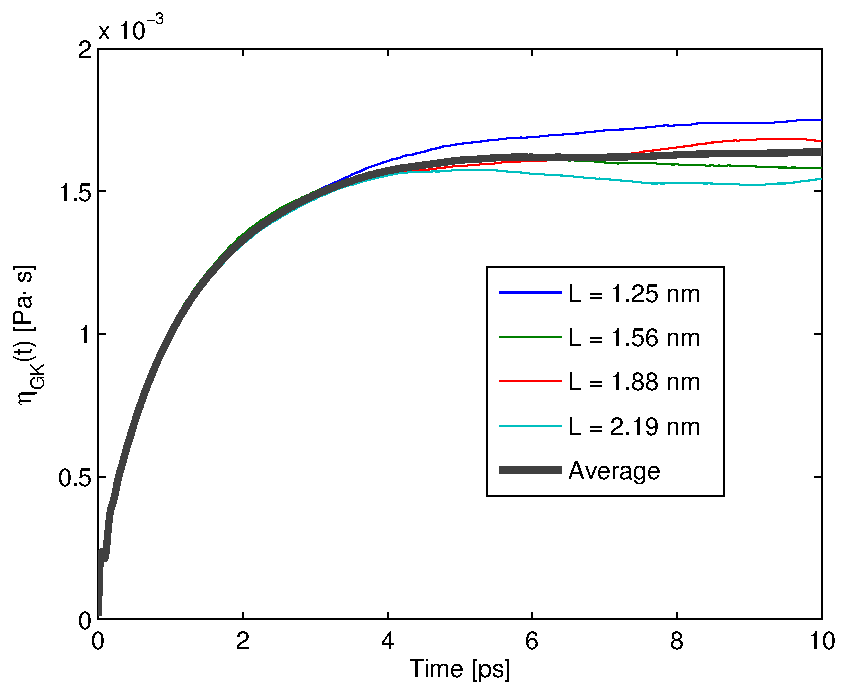
\includegraphics[width=11cm]{../figures/thesis/viscosity_green_kubo_tip4p_ice.pdf}
\caption{Shear viscosity for TIP4P/Ice at \SI{300}{\kelvin} and $\rho = \text{\SI{0.98}{\gram\per\cubic\cm}}$. Each thin line shows the average of the 5 independent pressure component. The thich line is the average of 4 independent simulations. The viscosity is estimated to $\eta_{GK} = \text{\SI{1.63\pm0.05}{\milli\pascal\second}}$}
\label{fig:viscosity_green_kubo_tip4p_ice}
\end{figure}

\begin{figure}
\centering
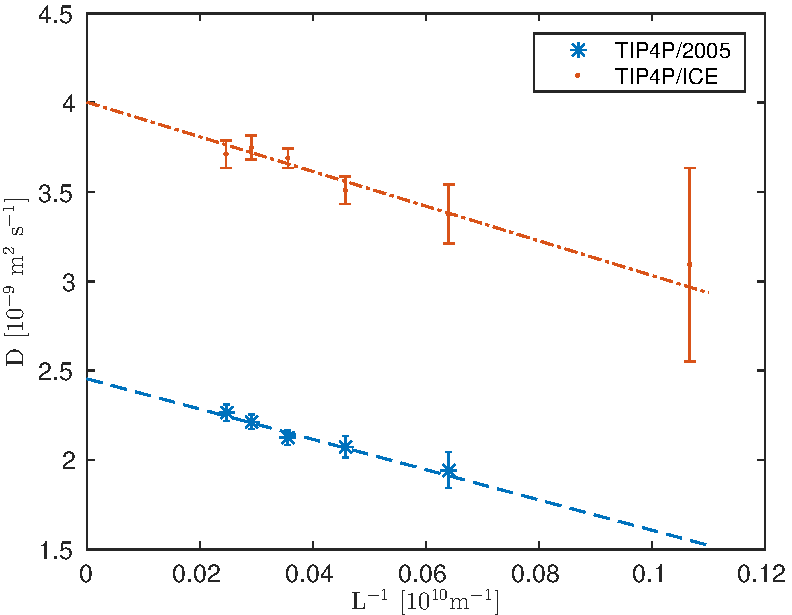
\includegraphics[width=11cm]{../figures/thesis/diffusivity_comparison_tip4p_ice_2005.pdf}
\caption{Linear regression of self diffusion coefficients as a function of inverse simulation box length. Results for TIP4P/2005 (blue) were already reported in the verification section. The self-diffusion coefficient for TIP4P/Ice is estimated to $D_0 = \SI{4.0 \pm 0.1 d-9}{\meter\squared\per\second}$}
\label{fig:diffusivity_comparison_tip4p_ice_2005}
\end{figure}

\section{Measuring elastic properties with a constant strain rate}
A simple approach to measuring elastic properties, which I will use for my estimates, is to subject a system to a constant strain rate by expanding the simulation box in one of the coordinate directions. Atom positions must be rescaled accordingly, to avoid the introduction of elastic waves. This is also justified by the fact that there are no ``special places'' in the simulation box -- since it is periodic in all directions -- so expanding the simulation box without rescaling the particle positions would be a strange choice. An anisotropic barostat will be applied along the other axes, to keep the confining pressure constant. The barostat will change dimensions of the simulation box perpendicular to the applied deformation, so the lateral strains can be measured using the dimensions of the simulation box:

\begin{equation}
\varepsilon_i = \frac{L_i-L_{0, i}}{L_{0, i}}
\end{equation}

If the sample is isotropic, strain application in only one of the coordinate directions has to be applied to estimate both Young's modulus and Poisson's ratio for a given system. To account for the possibility that the model I use do not exhibit isotropic behavior, I will deform the system in only \emph{one} direction, but check the resulting lateral strains in both of the coordinate directions perpendicular to the axis of applied strain. The value of Poisson's ratio,$\nu$, is minus the ratio of lateral to normal strain. For linear materials, this can be calculated as the negative of the slope of the strain-strain curve. The value of Young's modulus,$E$, is normal stress divided by normal strain. Again, this can be calculated as the slope of the stress--strain curve if the material is linear. I will calculate these slopes using linear regression with least squares on the curves, and check whether the slope is actually linear by visual inspection.

In the following, I apply the method described above to a Lennard-Jones crystal and to the TIP4P/Ice+UAM methane hydrate model.

\subsection{Lennard-Jones crystal}
The FCC-lattice with a Lennard-Jones potential has been extensively investigated due to its simplicity and its fundamental role in molecular dynamics. Therefore it provides robust benchmarking capabilities. I will check that my protocols for dynamic (but quasi-static) determination of elastic properties reproduce known parameters for a Lennard-Jones solid. Reference values are: Young's modulus, $E=61.1 \epsilon/\sigma^3$ ($ = \text{\SI{2.40}{\giga\pascal}}$ for the parameters I use for methane), and Poisson's ratio, $\nu=0.347$. These values are taken from a molecular dynamics study by \citet{Quesnel1993}.

The elastic test is performed on two Lennard--Jones systems of different size: 
One consisting of $11^3$ FCC unit cells, and another consisting of $22^3$ FCC unit cells. The samples are subjected to a strain rate of \SI{2d-8}{\per\femto\second} over \SI{0.4}{\nano\second}, resulting in a maximum strain of \SI{8d-3}{}. The external pressure is set to \SI{50}{\mega\pascal}, and the temperature is \SI{5}{\kelvin}. The stress--strain curve and the normal strain--lateral strain curves are shown in figures \ref{fig:stress_strain_11_11_11_and_22_22_22_y_z_poisson_lennard_jones} and \ref{fig:strain_strain_11_11_11_and_22_22_22_y_z_poisson_lennard_jones}, respectively. Estimates of Poisson's ratio and Young's modulus, taken as the best linear regression with least squares, are indicated in the figure legends. The data show no significant finite-size effects on the elastic properties. Young's modulus is estimated to $E = \SI{2.48}{\giga\pascal}$, and Poisson's ratio is estimated to $\nu = 0.35$. This corresponds well with the numbers reported by \citet{Quesnel1993}.

\begin{figure}
\centering
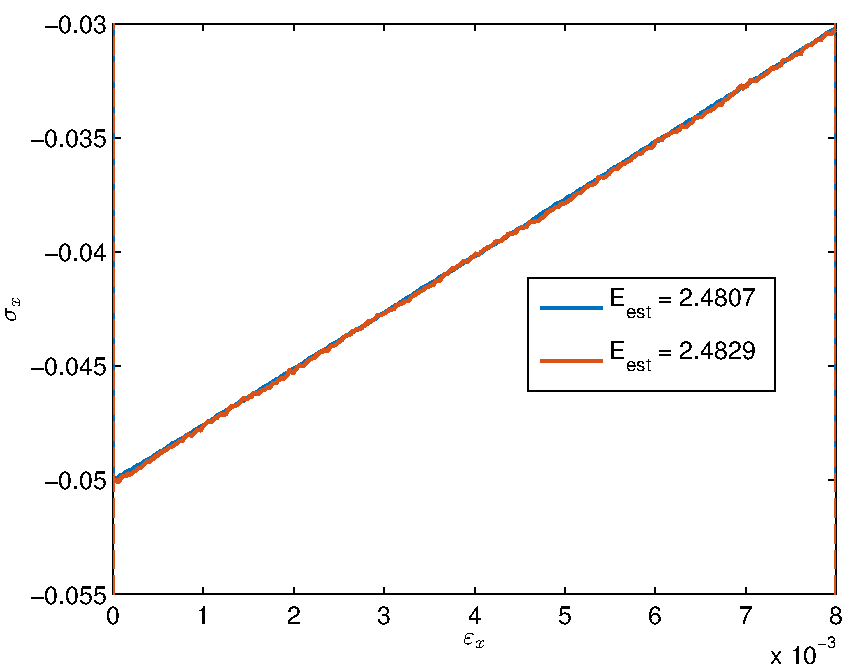
\includegraphics[width=11cm]{../figures/thesis/stress_strain_11_11_11_and_22_22_22_y_z_poisson_lennard_jones.pdf}
\caption{Stress-strain relations for Lennard-Jones systems of $11^3$ (red) and $22^3$ (blue) FCC unit cells. The sample was subjected to a constant strain rate of \SI{2d-8}{\per\femto\second}. Young's modulus, $E$, is estimated using linear regression with least squares on all data points.}
\label{fig:stress_strain_11_11_11_and_22_22_22_y_z_poisson_lennard_jones}
% Path to simulation: /media/henriasv/Data/molecular-data/master_methane_hydrates/stress_strain/20150113_lennard_jones_strain
\end{figure}

\begin{figure}
\centering
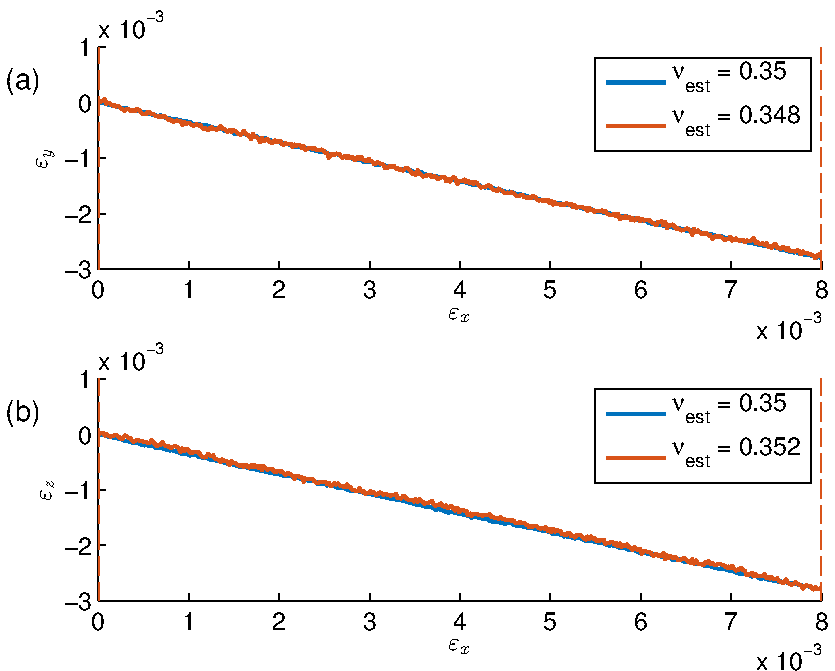
\includegraphics[width=11cm]{../figures/thesis/strain_strain_11_11_11_and_22_22_22_y_z_poisson_lennard_jones.pdf}
\caption{Strain-strain relations for for the same simulations as in Figure \ref{fig:stress_strain_11_11_11_and_22_22_22_y_z_poisson_lennard_jones}. All data points were used to estimate Poisson's ration,$\nu$.}
\label{fig:strain_strain_11_11_11_and_22_22_22_y_z_poisson_lennard_jones}
% Path to simulation: /media/henriasv/Data/molecular-data/master_methane_hydrates/stress_strain/20150113_lennard_jones_strain
\end{figure}

\subsection{sI methane hydrate with TIP4P/ICE+UAM}
To my knowledge, there are no published estimates of Young's modulus and Poisson's ratio for the TIP4P/Ice+UAM model of methane hydrates. Therefore, I seek to make crude estimates of these quantities in dynamic simulations. I perform the elastic test outlined above, with zero confining pressure. The test is performed on two systems of $11^3$ sI unit cells. One subjected to a strain rate of \SI{5d-7}{\per\femto\second}, and another subjected to a strain rate of \SI{2d-7}{\per\femto\second}. Having two simulations with a different strain rate, the calculated mechanical properties can be extrapolated to infinitely slow strain, yielding more accurate estimates.
Figure \ref{fig:stress_strain_11_11_11_tip4p_ice_uam} shows the stress--strain relationships and corresponding estimates of Young's modulus. By extrapolation, Young's modulus is estimated to $E = \SI{7.1}{\giga\pascal}$.
Figure \ref{fig:strain_strain_11_11_11_y_z_poisson_tip4p_ice_uam} shows the relationship between applied normal strain and the measured laterals strains. Based on the results shown in this figure, I find it reasonable to treat methane hydrates as isotropic for this work. My extrapolated estimate of Poisson's ratio is $\nu = 0.41$. Putting the calculated values for Young's modulus and Poisson's ratio, along with the density calculated from \citet{Ning2010}, $\rho = \SI{0.919}{\kilo\gram\per\liter}$, into the equations for shear and pressure waves, give the elastic wave speeds for the methane hydrate: $v_s=\SI{3780}{\meter\per\second}$ and $v_p = \SI{1650}{\meter\per\second}$. From the Poisson's ratio and the shear wave speed, the Rayleigh wave speed can be calculated using the following approximate formula from \cite{0957-4484-16-6-N01}:
\begin{equation}
v_R = v_s(0.874 + 0.196\nu − 0.043\nu^{2} − 0.055\nu^{3}),
\end{equation}
This results in a Rayleigh wave speed of $v_R = \SI{1570}{\meter\per\second}$.
The new mechanical properties obtained for methane hydrates in the TIP4P/Ice + UAM model in this work are given in table \ref{tbl:mechanical_from_simulation}. Compared to the experimental values I presented in table \ref{tbl:si_mech_exp}, these mechanical properties are quite good, except from Poisson's ratio which differs quite significantly from the experimental value.
\begin{table}
\centering
\caption{Mechanical properties of the methane hydrate in the TIP4P/Ice + UAM model measured under isothermal tensile strain with zero confining pressure. The elastic wave speeds are derived from Young's modulus and Poisson's ratio.}
\label{tbl:mechanical_from_simulation}
\begin{tabular}{c|c}
Property & Value \\
\hline
Young's modulus, $E$ & \SI{7.1}{\giga\pascal} \\
Poisson's ratio, $\nu$ & 0.41 \\
Shear wave speed, $v_s$ & \SI{3780}{\meter\per\second} \\
Pressure wave speed $v_p$ & \SI{1650}{\meter\per\second} \\
Rayleigh wave speed $v_R$ & \SI{1570}{\meter\per\second} \\
\end{tabular}
\end{table}

\begin{figure}
\centering
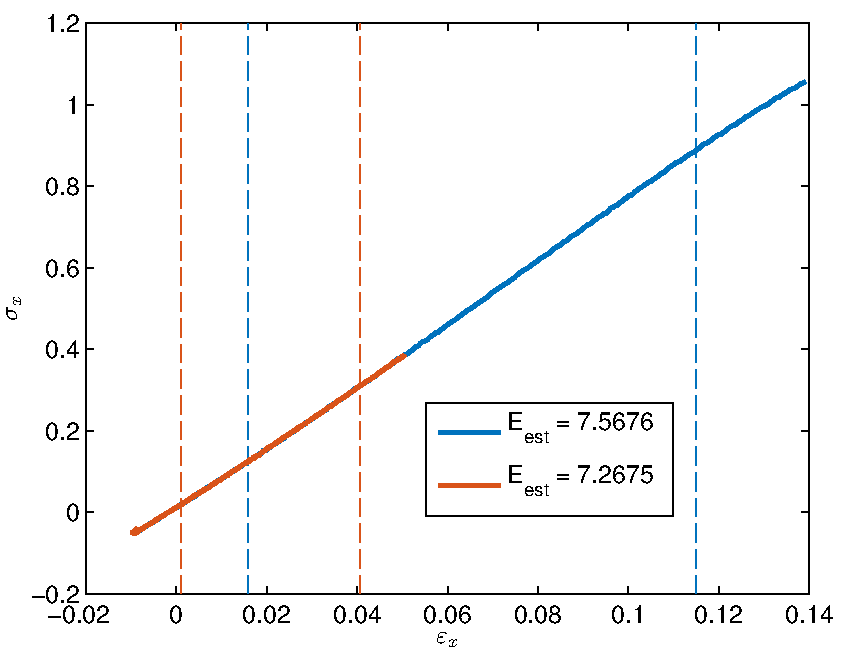
\includegraphics[width=10cm]{../figures/thesis/stress_strain_11_11_11_tip4p_ice_uam.pdf}
\caption{Stess--strain relations for a system of 11x11x11 sI unit cells. Dashed lines indicate the region that was used to estimate Young's modulus. Strain rates of \SI{5d-7}{\per\femto\second} (blue) and \SI{2d-7}{\per\femto\second} (red) along the x-axis. Upon close visual inspection, a slight rising slope can be seen for small strains and a rising slope for large strains, but overall the stress-strain relation is surprisingly linear, especially given the large strain-range.}
\label{fig:stress_strain_11_11_11_tip4p_ice_uam}
% Path to simulation: /media/henriasv/Data/molecular-data/master_methane_hydrates/stress_strain/20150108_youngs_modulus

\end{figure}

\begin{figure}
\centering
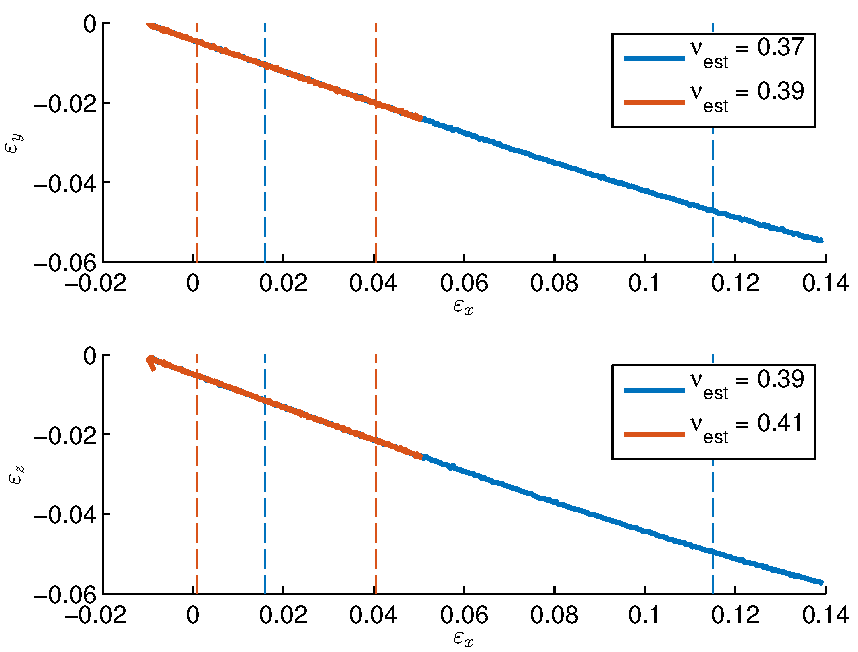
\includegraphics[width=10cm]{../figures/thesis/strain_strain_11_11_11_y_z_poisson_tip4p_ice_uam.pdf}
\caption{Strain-strain relations for the same system as in Figure \ref{fig:stress_strain_11_11_11_tip4p_ice_uam}. Measured strain along the y-axis (a) and z-axis (b) is plotted against the applied strain along the x-axis. Dashed lines indicate the region that was used to estimate Poisson's ratio.}
\label{fig:strain_strain_11_11_11_y_z_poisson_tip4p_ice_uam}
% Path to simulation: /media/henriasv/Data/molecular-data/master_methane_hydrates/stress_strain/20150108_youngs_modulus

\end{figure}

\section{Early results on fracture and fracture toughness}
Having obtained the basic elastic properties, I go on to the fracture studies. I start by discussing the simulation protocol for fracture simulations, and  continue by performing preliminary simulations to verify that the protocol works. The main goal I work towards here, is to calculate the fracture toughness of methane hydrates.
\subsection{Simulation protocol}
Several approaches can be applied to determine the fracture toughness in molecular dynamics. \citet{Hantal2014}performed NVT simulations and imposed incremental deformations to their sample. After each deformation, they minimized the system, and then ran molecular dynamics for \SI{10}{\pico\second}. I tried to use the same protocol, but found that for my system, the impact on the energy distribution among the degrees of freedom was too large when performing minimizations between the deformations. After a deformation, the system is no longer in equilibrium, and the minimization is supposed to bring the system closer to equilibrium. However, in an equilibrium of finite temperature, some fraction of the system energy is associated with moving particles being temporarily positioned closer or farther from each other than the equilibrium distance dictated by their inter-atomic potential and the overall structure of the system. This is a thermal energy. A minimization removes this energy from the system, and when an NVT simulation is started after minimization, the thermostat will have to put this energy back into the system. This takes time: With the thermostat settings I apply, it takes several tens of picoseconds. Therefore, a possible protocol that does not use minimization is:
\begin{enumerate}
\item Carve out an initial crack and equilibrate the system NPT to relax the system after the crack is introduced.
\item Perform small deformation
\item Re-equilibrate the system NVT.
\item Molecular dynamics run (NVT) to wait for failure
\item Return to 2 or end the simulation. 
\end{enumerate}
This approach was also tested, but it turned out that the waiting times were unpredictable -- it was hard to set a reasonable waiting time for step 4. This resulted in additional deformations being applied \emph{during} fracture. 
%
\begin{framed}
\textbf{The protocol I will actually use:} A simpler protocol -- and I believe this to be a good way to study this particular system -- is to subject the sample to a constant strain rate until it reaches some predefined strain, and then wait for a crack to propagate. This is simple to do, and it is also close to experimental conditions, except that the strain rate must necessarily be much higher in MD simulations than in experiments. The downside of this method is that only a single strain level will be tested in each simulation, but if there exists waiting times for fracture that depend on the applied strain, then there has to be performed individual simulation for each strain level anyway.
\end{framed}

In addition to complication the simulations, I see the possible waiting times for fracture as a research opportunity. Waiting times for fracture can depend for example on the applied strain and temperature, and this relation can be characterized. It will probably be very computationally demanding to obtain good statistics, but I believe that some tendencies can be identified without spending too many CPU-hours.

%%%%%%%%%%%%%%%%%%%%%%%%%%%%%%%%%%%%%%%%%%%%%%%%%%%%%%%%%%%%%
\subsection{Proof-of-concept simulations}
%%%%%%%%%%%%%%%%%%%%%%%%%%%%%%%%%%%%%%%%%%%%%%%%%%%%%%%%%%%%%
Before performing large scale simulations, I do preliminary, smaller, simulations to find out whether the protocol proposed in the latter section can produce useful results. I do simulations on the thinnest possible system consisting of sI unit cells -- the system that is only one unit cell thick -- to keep computational costs down. The total computational cost for tuning in on parameters and getting rid of bugs and blunders has been around $10^4$ CPU hours.

The proof-of-concept simulations are performed using the protocol outlined above (the one that I state I will be using), on systems of $24\times 24\times 1$ sI methane hydrate unit cells. The systems are subjected to a constant strain rate during \SI{50}{\pico\second}, to obtain a strains ranging from 0.045 to 0.1. Then, the system is left on its own. Table \ref{tbl:proof_of_concept_parameters} shows all parameters of these simulations.

The simplest way to identify whether a crack has propagated, it turns out, is to check the potential energy curve. The potential energy of the system goes down when the system fractures. Figure \ref{fig:proof_of_concept_crack} shows the potential energy of the proof-of-concept simulations. In three of the systems, a crack spans the $yz$-plane after the simulation is finished. In one of the simulations, no crack growth is observed.

Below is a description of the visual experience of the crack propagation in one of the simulations:

\begin{table}
\caption{Parameters for the proof-of-concept simulations.}
\label{tbl:proof_of_concept_parameters}
\begin{tabular}{|rl|}
\hline
System & $24\times 24 \times 1$ sI unit cells. Initialized with crack of $6\times \SI{40}{\angstrom}$\\
Protocol:& 0--\SI{100}{\ps}: NPT @ \SI{101325}{\pascal}, \SI{260}{\kelvin} \\
& 100--\SI{150}{\pico\second}: NVT @ \SI{260}{\kelvin} with straining \\
& 150--\SI{550}{\pico\second}: NVT @ \SI{260}{\kelvin} and final strain \\
Final strain: & [1.045, 1.05, 1.055, 1.1] \\
Interactions: & TIP4P/Ice and United Atom Methane \\
Short-range potentials: & Lennard--Jones and Coulomb with \SI{10}{\angstrom} cutoff. \\
Long-range corrections: & Coulomb with P$^3$M allowing a relative error of $10^{-4}$. \\
Thermostat damping time: & \SI{1}{\pico\second} \\
Barostat damping time: & \SI{1}{\pico\second} \\
Integration timestep: & \SI{1}{\femto\second} \\ 
SHAKE tolerance: & $10^{-4}$ \\
Drag term (LAMMPS specific): & 1.0 \\
\hline
\end{tabular} 
\end{table}


\begin{framed}
\paragraph{Visual experience of the crack propagation (figure \ref{fig:thin_crack})}
First, the system slightly contracts (NPT allows volume change). The system comes to rest, and some methane molecules diffuse out of near-wall cages to the hole that was carved out during initialization. After \SI{100}{\pico\second} straining starts. The system expands to 1.05 times its original length along the x-axis at a constant rate during \SI{50}{\pico\second}. This corresponds to a very high strain rate in macroscopic terms. More methane fills the crack, as its volume increases when the crack gets wider -- but the crack length remains the same during expansion. The system has now reached is the desired strain. Methane molecules bounce back and fourth inside the crack, and the crack edges seem jittery. Suddenly, a hydrogen bond near a crack tip breaks -- fluctuations from methane molecules and lattice vibrations have made the system unstable. When the first bond breaks, the next bond along the crack axis cannot sustain the stress. Bonds near the other crack edge breaks. Then bonds break one after the other on both edges of the crack -- the crack propagates. In a matter of tens of picoseconds, both crack edges reach the periodic boundary. During crack propagation, clathrate cages are ripped apart. Water molecules remain stuck to the wall, while methane is released, and fills the void between the two pieces of methane hydrate (To be more precise, there is still only one piece of methane hydrate because of the periodic boundaries). The crack is not traveling straight in one direction: It first starts traveling between columns of sI cells before it turns and continues to propagate in the middle of hydrate cells, ripping apart big cages. Just after the crack has propagated, the methane hydrate oscillates with a spatial amplitude comparable to the void width. During the following hundreds of picoseconds, the oscillations damp out -- the system is approaching a new equilibrium.
\end{framed}

\begin{figure}
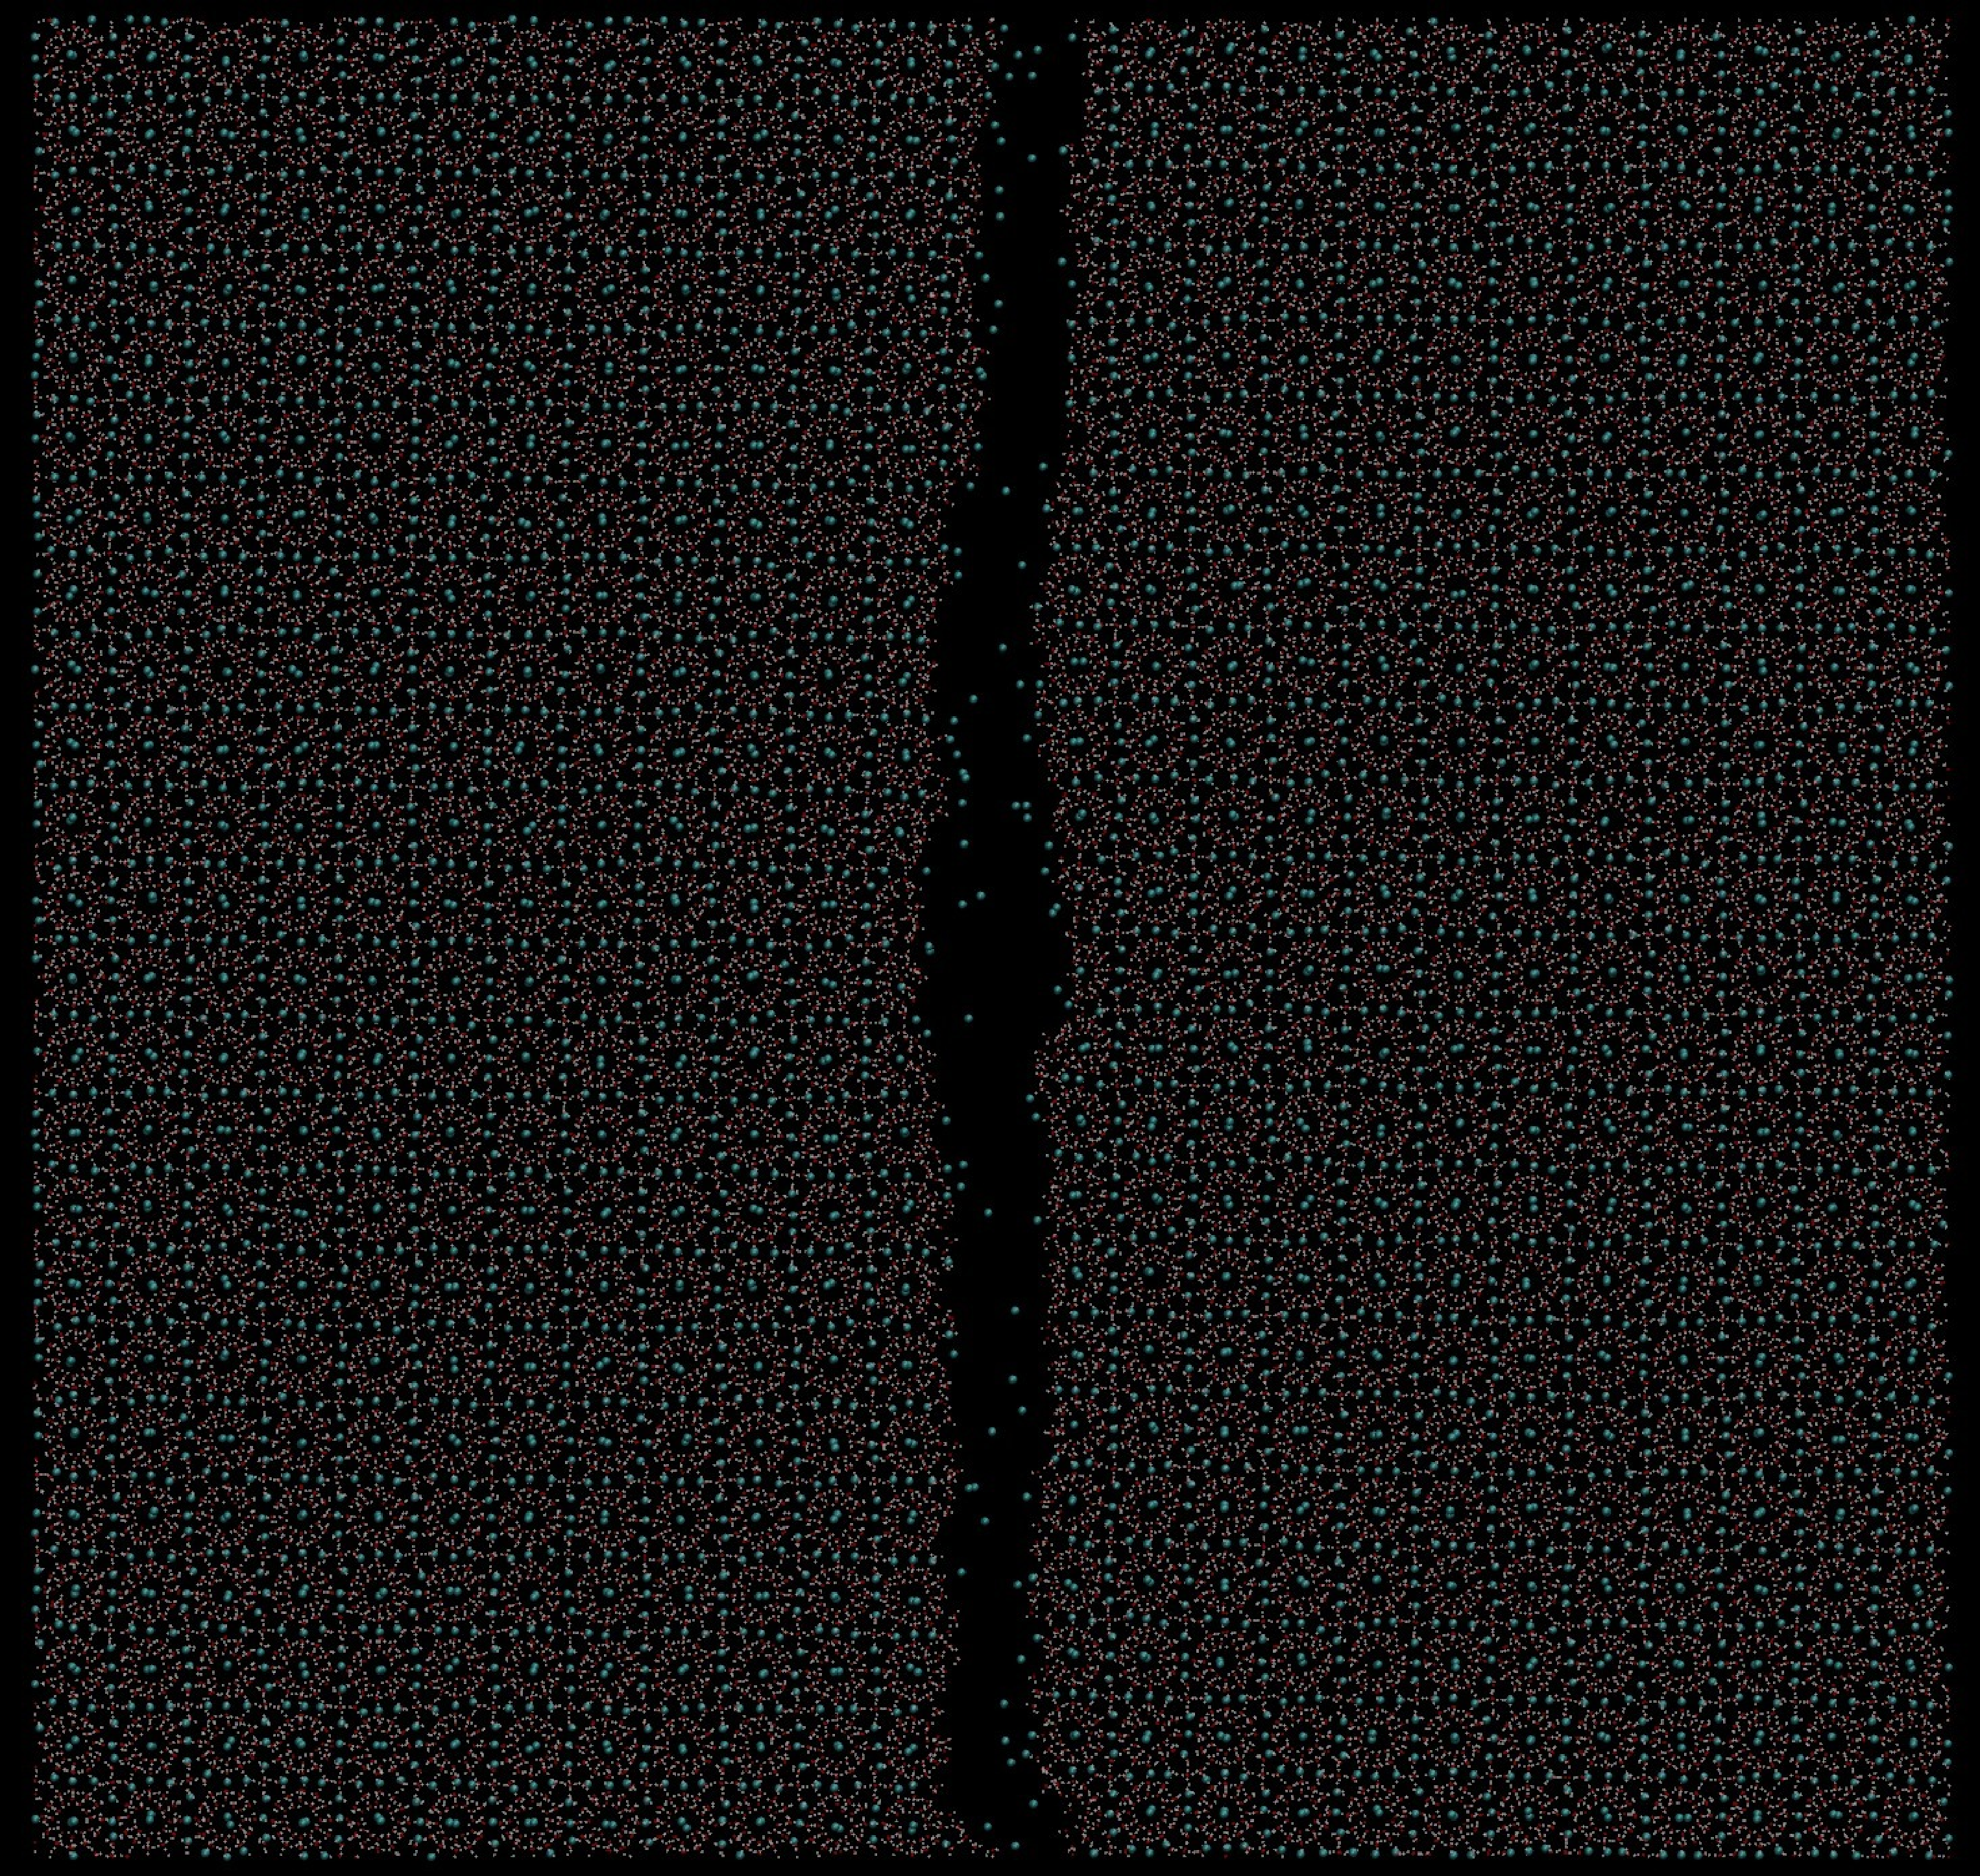
\includegraphics[width=\textwidth]{../pictures/slim_system.pdf}
\caption{Fracture of a system of $24 \times 24 \times 1$ sI unit cells. The upper crack changes from propagating between columns of unit cells to propagating in the middle of a column of unit cells, breaking big cages instead of small ones.}
\label{fig:thin_crack}
\end{figure}

From the visuals, I move on to preliminary calculations of the surface energy and the critical energy release rate. The surface energy can be estimated as the change in potential energy from the equilibrated system before straining to the system of methane hydrate and free methane after crack propagation. The energy release rate can be estimated as the change in potential energy during crack propagation. If $\Delta U_c$ is the change in potential energy during crack propagation, and $\Delta U_s$ is the change in potential energy from before straining to after crack propagation, then the formulas for $G_c$ and $\gamma_s$ read:

\begin{equation}
	\mathcal{G}_c \approx \frac{\Delta U_c}{L_yL_z}
\end{equation}

\begin{equation}
	\gamma_s \approx \frac{\Delta U_s}{2 L_y L_z}
\end{equation}
%
Where the $\frac{1}{2}$ factor is because the crack opens two surfaces. The thermalization for all four of the simulations are equal, with an average potential energy of $\SI{-2.8112}{\femto\joule}$ on the plateau (40--100 \si{\pico\second}). The average potential energy after crack propagation is $\SI{-2.7970}{\femto\joule}$, with almost no variation between the simulations. This yields an energy difference of \SI{1.42d-17}{\joule}. Using the simulation box cross-sectional area (measured values: $L_y = \SI{288.8}{\angstrom}$, $L_z = \SI{12.04}{\angstrom}$) as an estimate of the crack size, the estimated surface energy is $\gamma_s = \SI{0.204}{\joule\per\meter\squared}$. Since the energy level required to start a crack is not well defined from figure \ref{fig:proof_of_concept_crack}, the estimate of the critical energy release rate is coarser than that of the surface energy. From the figure, I read off a potential energy of around \SI{-2.765}{\femto\joule} from the simulation that needed the least strain to produce a system-spanning crack. The estimated critical energy release rate from this potential energy is \SI{1.3}{\joule\per\meter\squared}. This corresponds to, using equation \ref{eq:energy_release_to_stress_intensity_isotropic} for the stress intensity in isotropic materials, a critical stress intensity factor of $K_{Ic} = 0.11 \text{ MPam}^{\frac{1}{2}}$ (Using $E=\SI{7.1}{\giga\pascal}$ and $\nu = 0.41$). Unfortunately, we shall see that this method for finding the fracture toughness is wrong, because of how the energy was measured. This will be discussed and corrected later in this chapter. For reference, the experimental fracture toughness of freshwater ice is around $K_{Ic} = 0.10 \text{ MPam}^{\frac{1}{2}}$ \cite{benham1996mechanics}. 

\begin{figure}
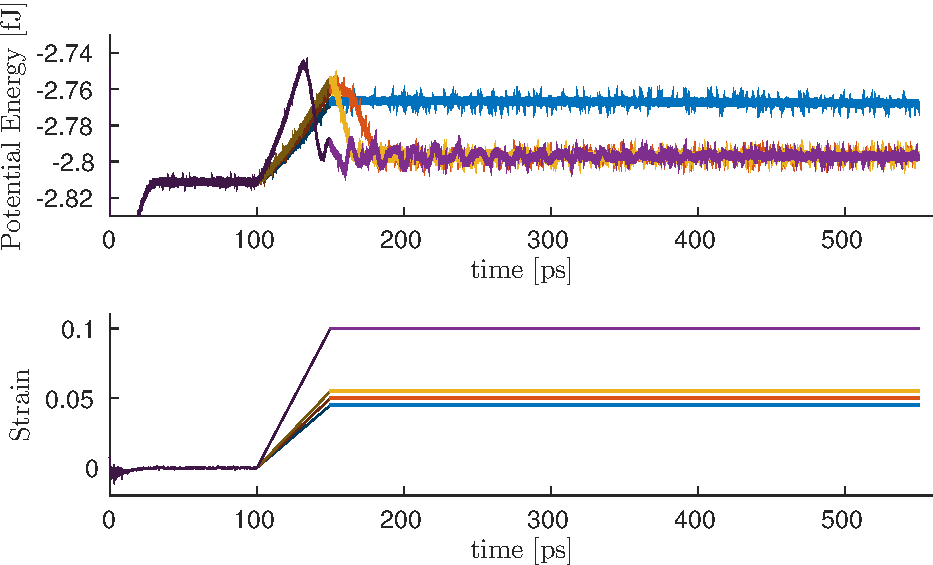
\includegraphics[width=\textwidth]{../figures/thesis/proof_of_concept_poteng_strain.pdf}
\caption{Potential energy (upper panel) and strain (lower panel) for a series of simulations where systems of $24\times 24\times 1$ unit cells of sI methane hydrate were subjected to tensile strain. The systems were initiated with an elliptic crack of $6.0 \times 40.0 \si{\angstrom}$. The system was then allowed to equilibrate NPT during \SI{100}{\pico\second}, which can be seen from the small fluctuations in strain in this time-frame. Then the simulations were continued NVT, but with an imposed volume change due to the application of a constant strain rate in the $x$-direction, taking the system to a predesignated stress after \SI{50}{\pico\second} of straining. Then, a regular NVT-simulation was run for \SI{400}{\pico\second} (bright colors). The thermostat and barostat damping times were \SI{1}{\pico\second}. $T=\SI{260}{\kelvin}$. Rapidly falling potential energies are due to crack opening. The slope of falling potential energy is systematically steeper for higher values of the strain before crack propagation. The systems that fracture show an oscillating potential energy after crack propagation, which is due to global oscillations of the system. The oscillations are damped out by a drag term in the thermostat. (The parameters of this simulation are also given in table \ref{tbl:proof_of_concept_parameters}.)}
\label{fig:proof_of_concept_crack}
\end{figure}

\paragraph{Detailed crack analysis}
The estimate of the surface area of the crack based on the simulation box side, is a rough estimate. I therefore decided to develop an improved measure of the crack area using a tailored algorithm and my own code. This algorithm was described in chapter \ref{ch:tools}. Hopefully, that estimate will be better than the estimate solely based on the simulation box dimensions. The code also lets me follow the crack area in time, which makes it possible to measure the crack speed. I choose to define the crack speed as the change of crack area divided by the crack depth, i.e. the length of the simulation box in the $z$-direction, $L_z$. Keeping in mind that my cracks travel in two directions, and that the crack opens two surfaces, the crack tip velocity of the crack that was initially cut as an elliptical prism with its axis in the $z$-direction becomes:

\begin{equation}
v_c = \frac{1}{2L_z}\frac{\dd A_c}{\dd t}
\end{equation}
%
Where $A_s$ is the measured crack surface area. Figure \ref{fig:crack_in_time_thin} shows the evolution of the crack area and crack speed in time in one of the proof-of-concept simulations, using a standard 5-point stencil to calculate the derivative of the crack surface area.
\begin{figure}
\centering
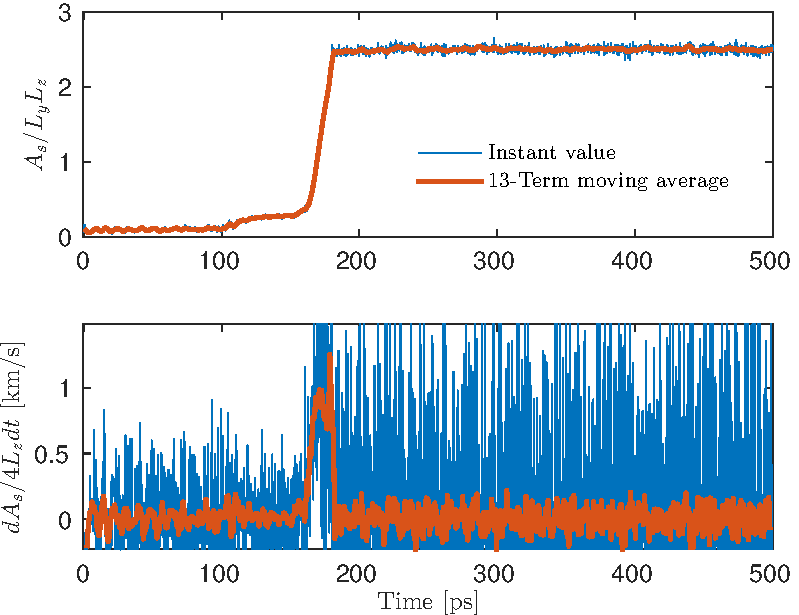
\includegraphics[width=12cm]{../figures/thesis/crack_in_time_thin.pdf}
\caption{Evolution of crack area in time (upper panel) and derived crack tip speed (lower panel).}
\label{fig:crack_in_time_thin}
\end{figure}

\paragraph{Summary of concept simulations} The results from these initial simulations indicate that methane hydrates are very brittle on the tens-of-picoseconds scale, in the sense that they do not at all deform plastically to withstand strain. They either deform elastically, or they fail. There is also indications that the time before fracture depends on the applied strain in a systematic way. A close look at the potential energy curve of the simulation in figure \ref{fig:proof_of_concept_crack} that did not end in rupture reveals that the potential energy is actually slowly decreasing. Whether this is a sign of a coming fracture, strengthening rearrangements of particles -- which could imply some ductility -- or something else, remains to be investigated. 

\paragraph{Observation of special feature -- a cavity in front of the crack tip}
Later on, I performed a few simulations with the same setup as in the proof-of-concept simulations, but with other levels of the final strain. In one of these simulations, one with a final strain of 0.046, I discovered a strange feature: A cavity formed in front of the initial crack. The crack did not go on to develop rapidly within the total simulation time of \SI{550}{\pico\second}, so I continued the simulation to see if it would develop further with time. It turned out that this simulation only needed a few tens of picoseconds to develop a system-spanning crack. Pictures of the time evolution of this crack is shown in figure \ref{fig:cavity_crack}. Cavities in front of the major crack has been discussed by for example \citet{Bouchbinder2004}.

\begin{figure}
\begin{minipage}[b]{0.19\linewidth}
\subcaptionbox{$t=\SI{300}{\pico\second}$}{
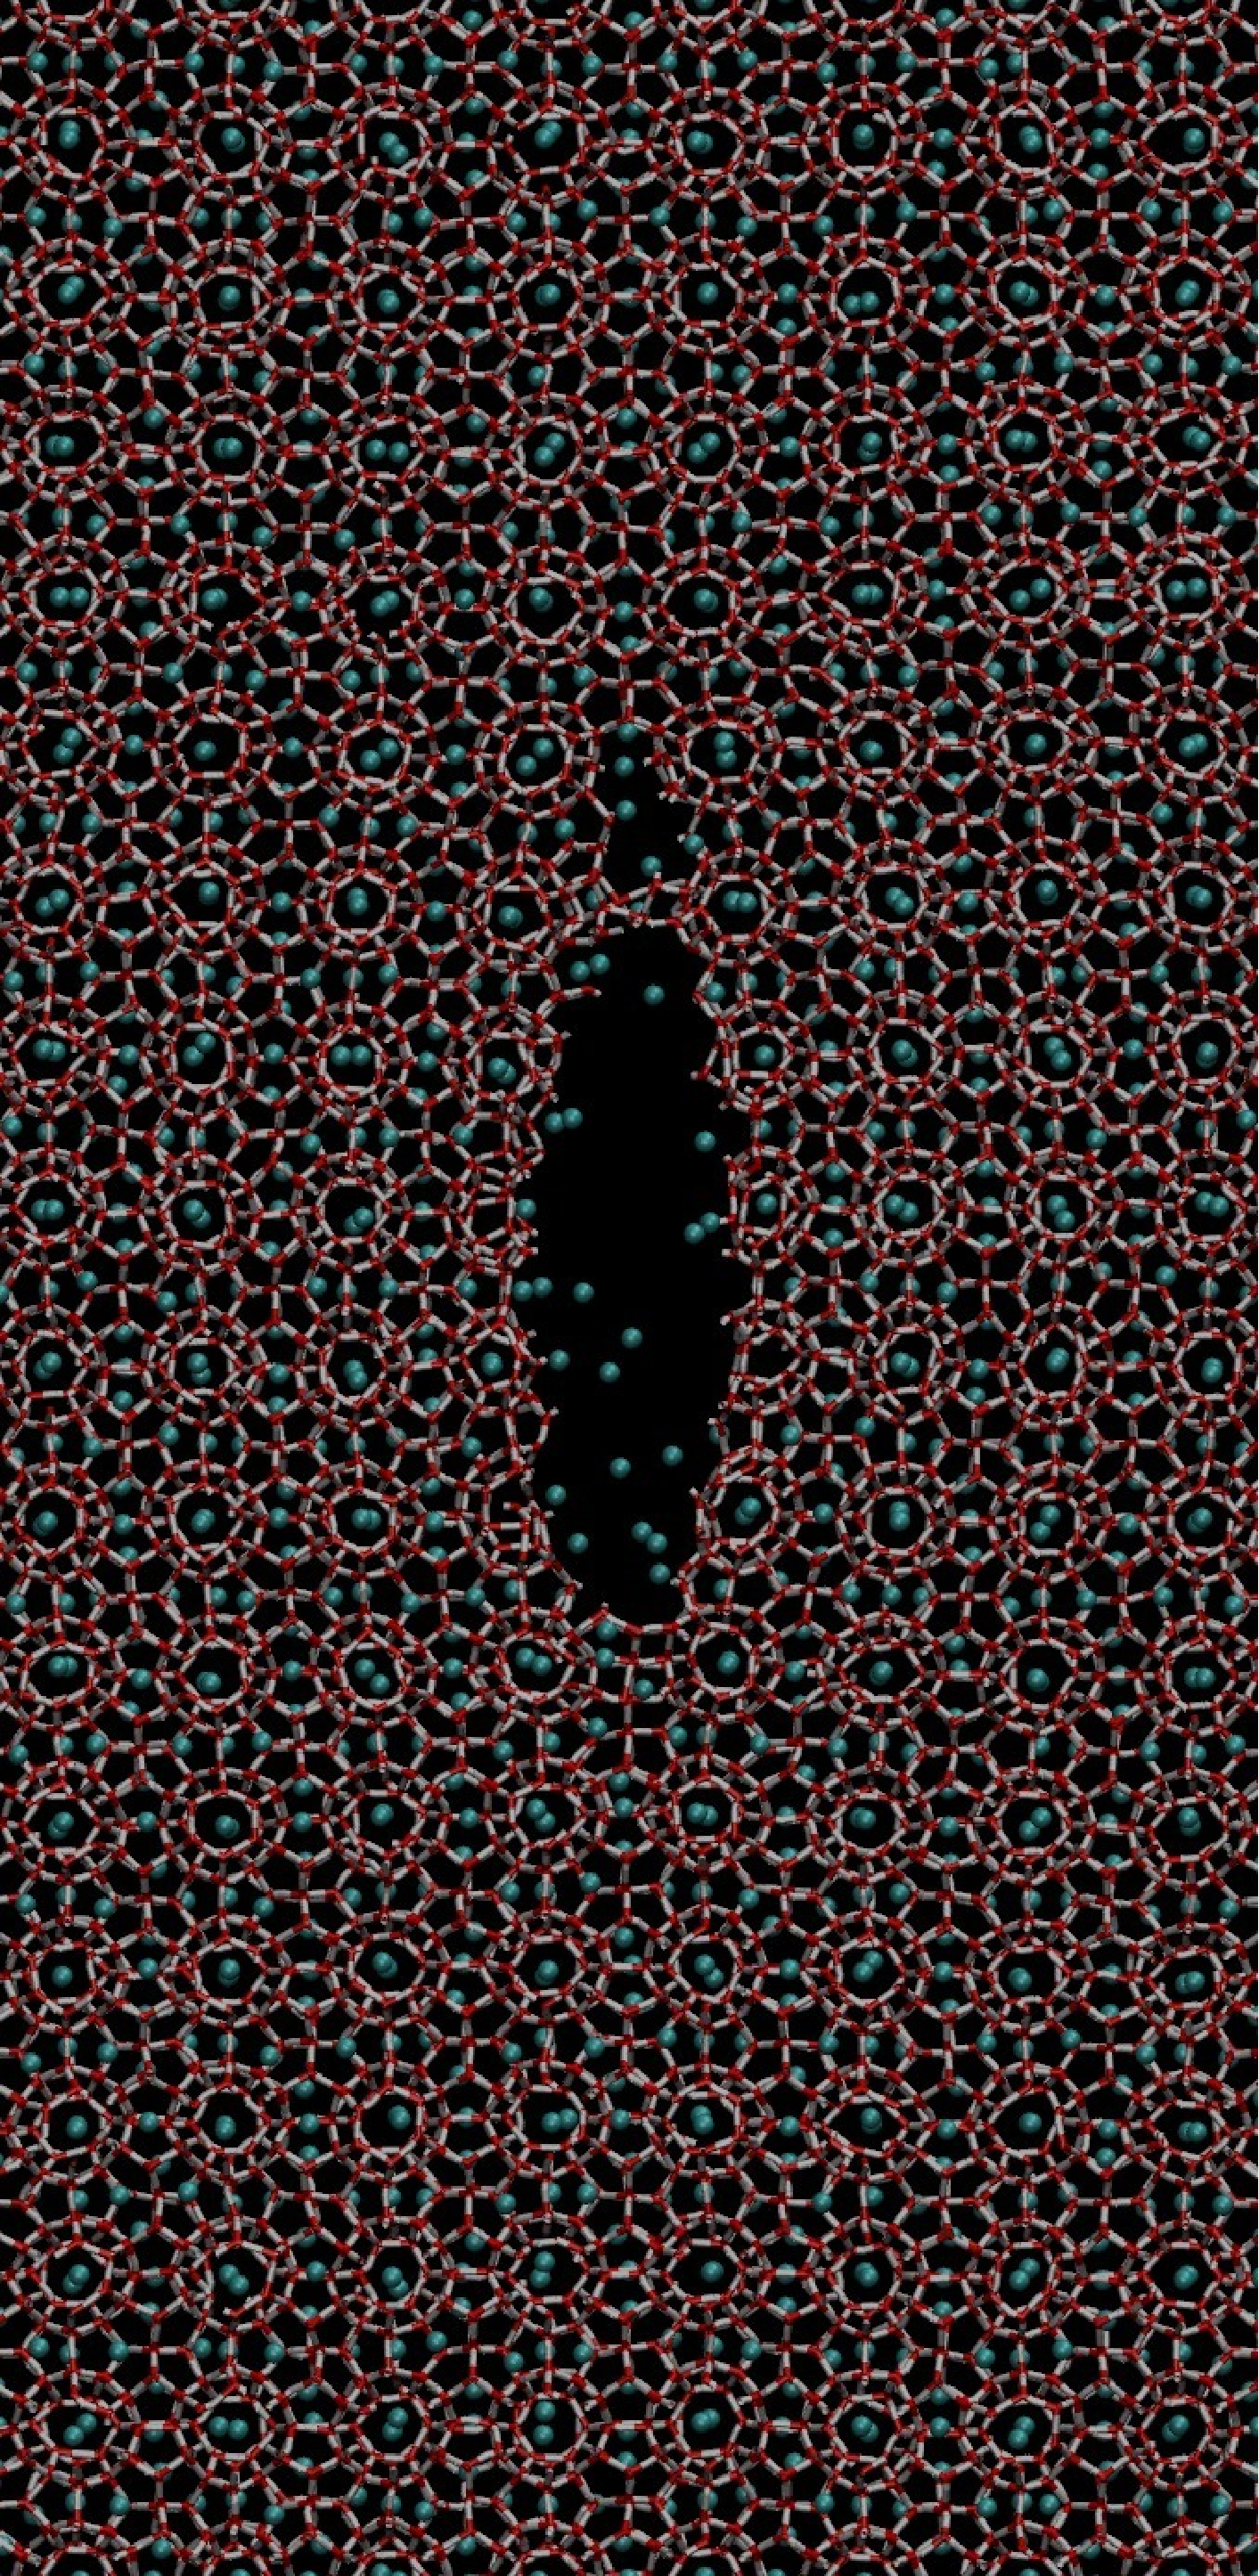
\includegraphics[width=\textwidth]{../pictures/snapshots_cavity_crack/at_300ps.pdf}}
\end{minipage}
\begin{minipage}[b]{0.19\linewidth}
\subcaptionbox{$t=\SI{540}{\pico\second}$}{
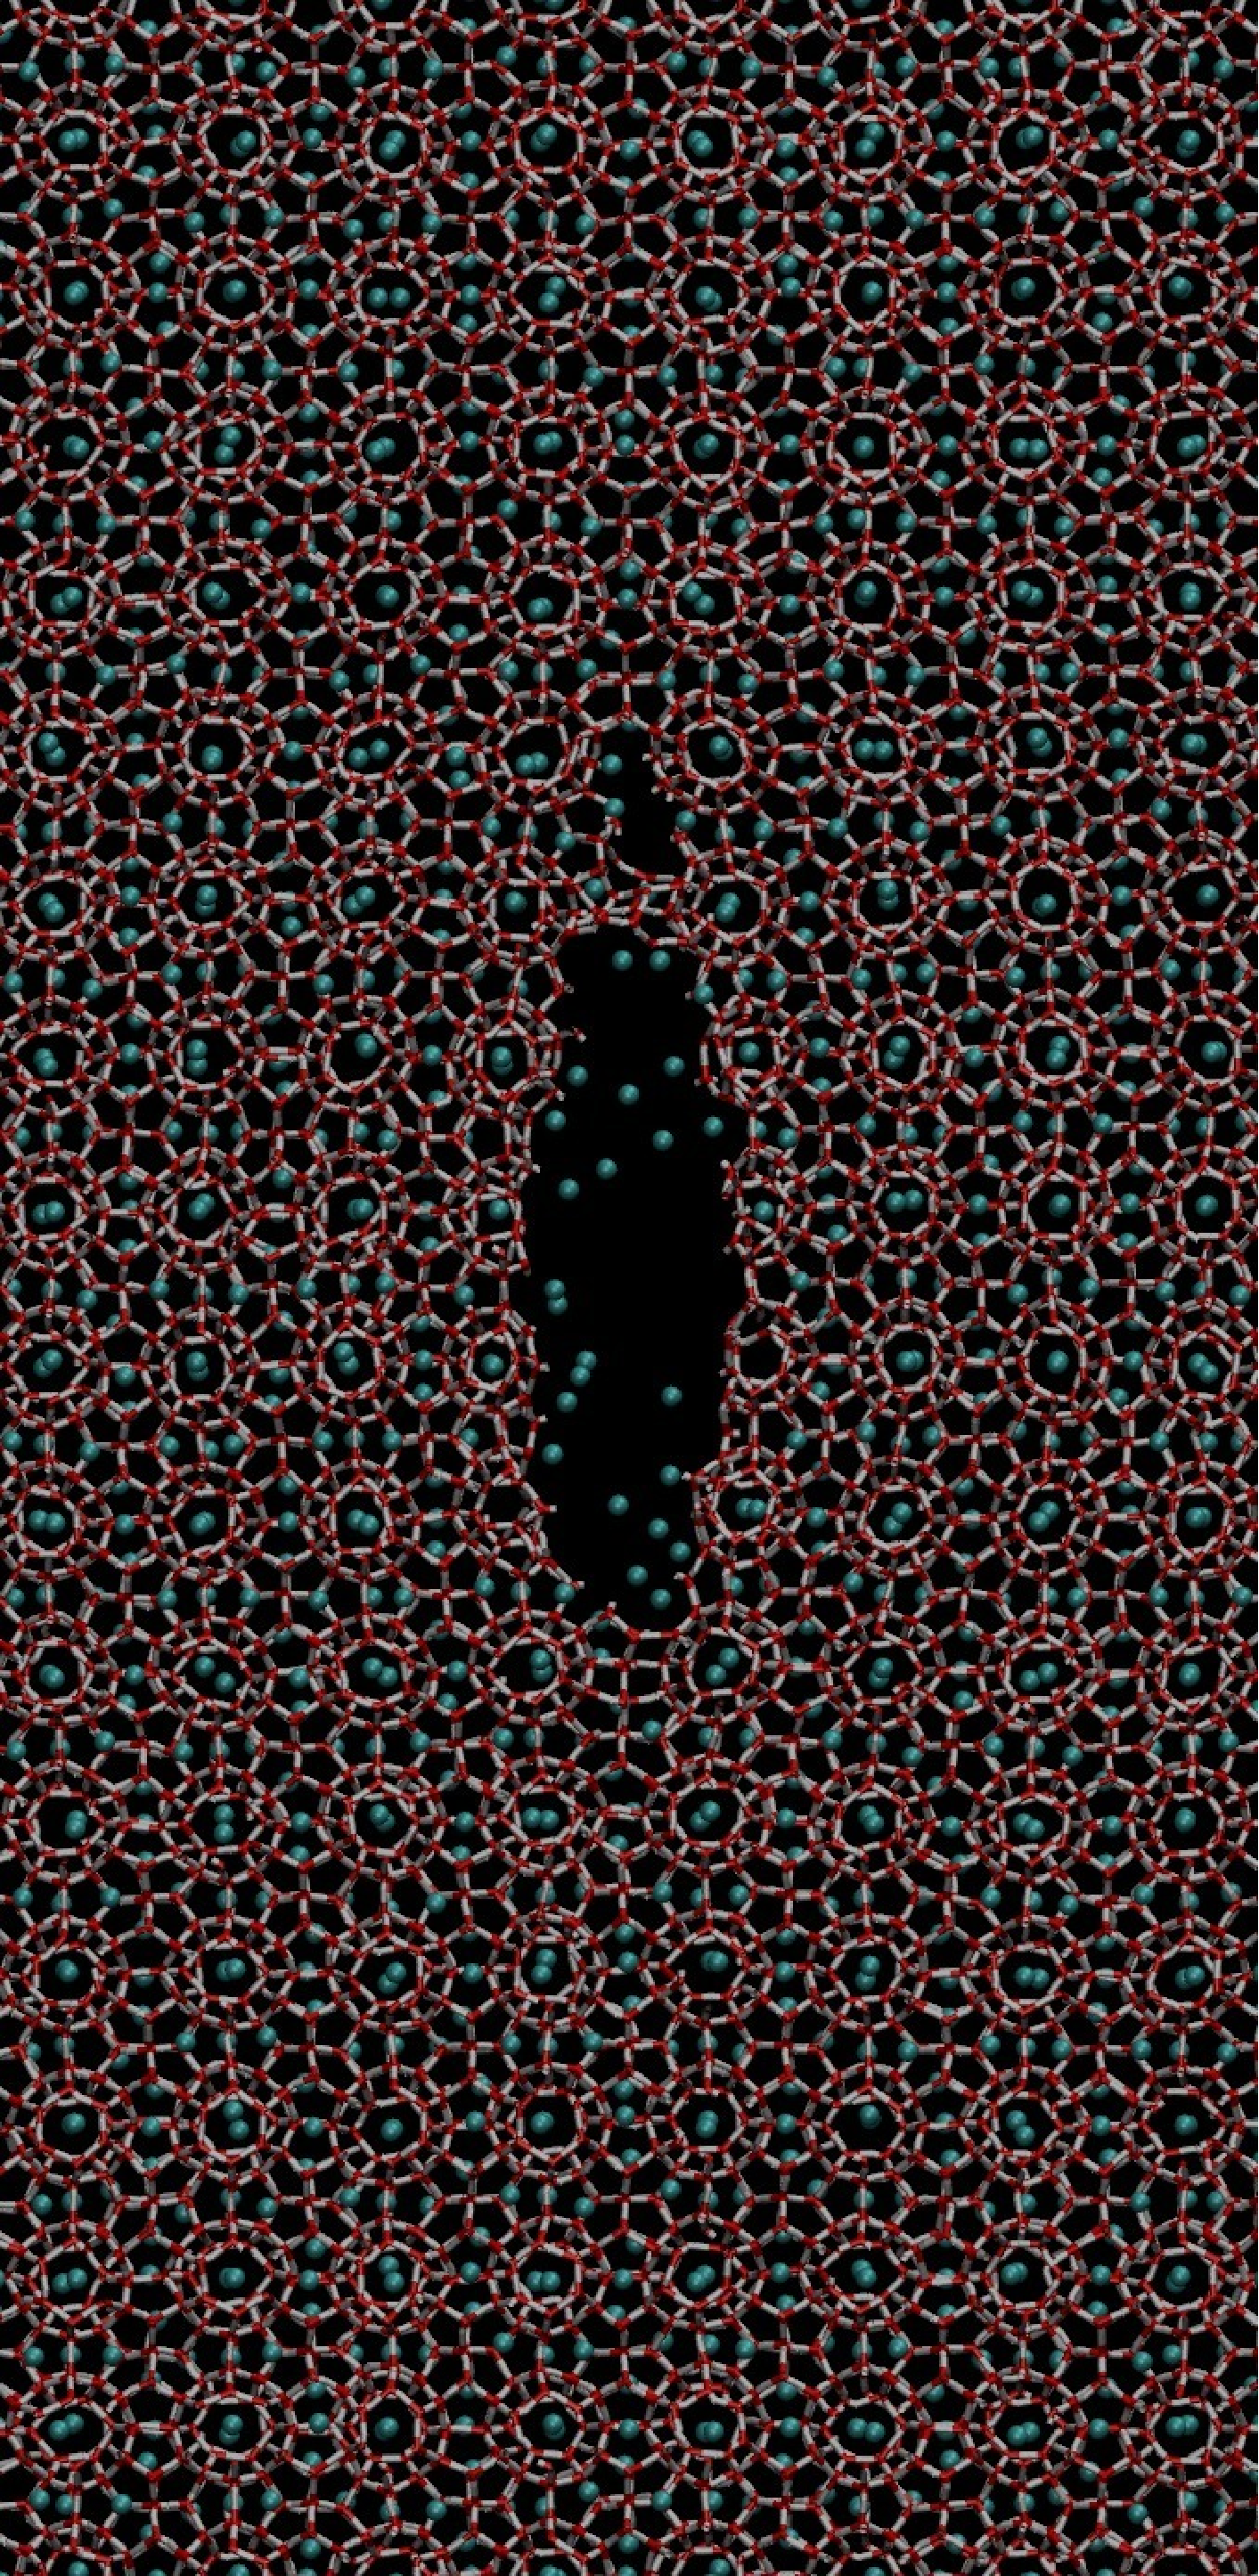
\includegraphics[width=\textwidth]{../pictures/snapshots_cavity_crack/at_540ps.pdf}}
\end{minipage}
\begin{minipage}[b]{0.19\linewidth}
\subcaptionbox{$t=\SI{555}{\pico\second}$}{
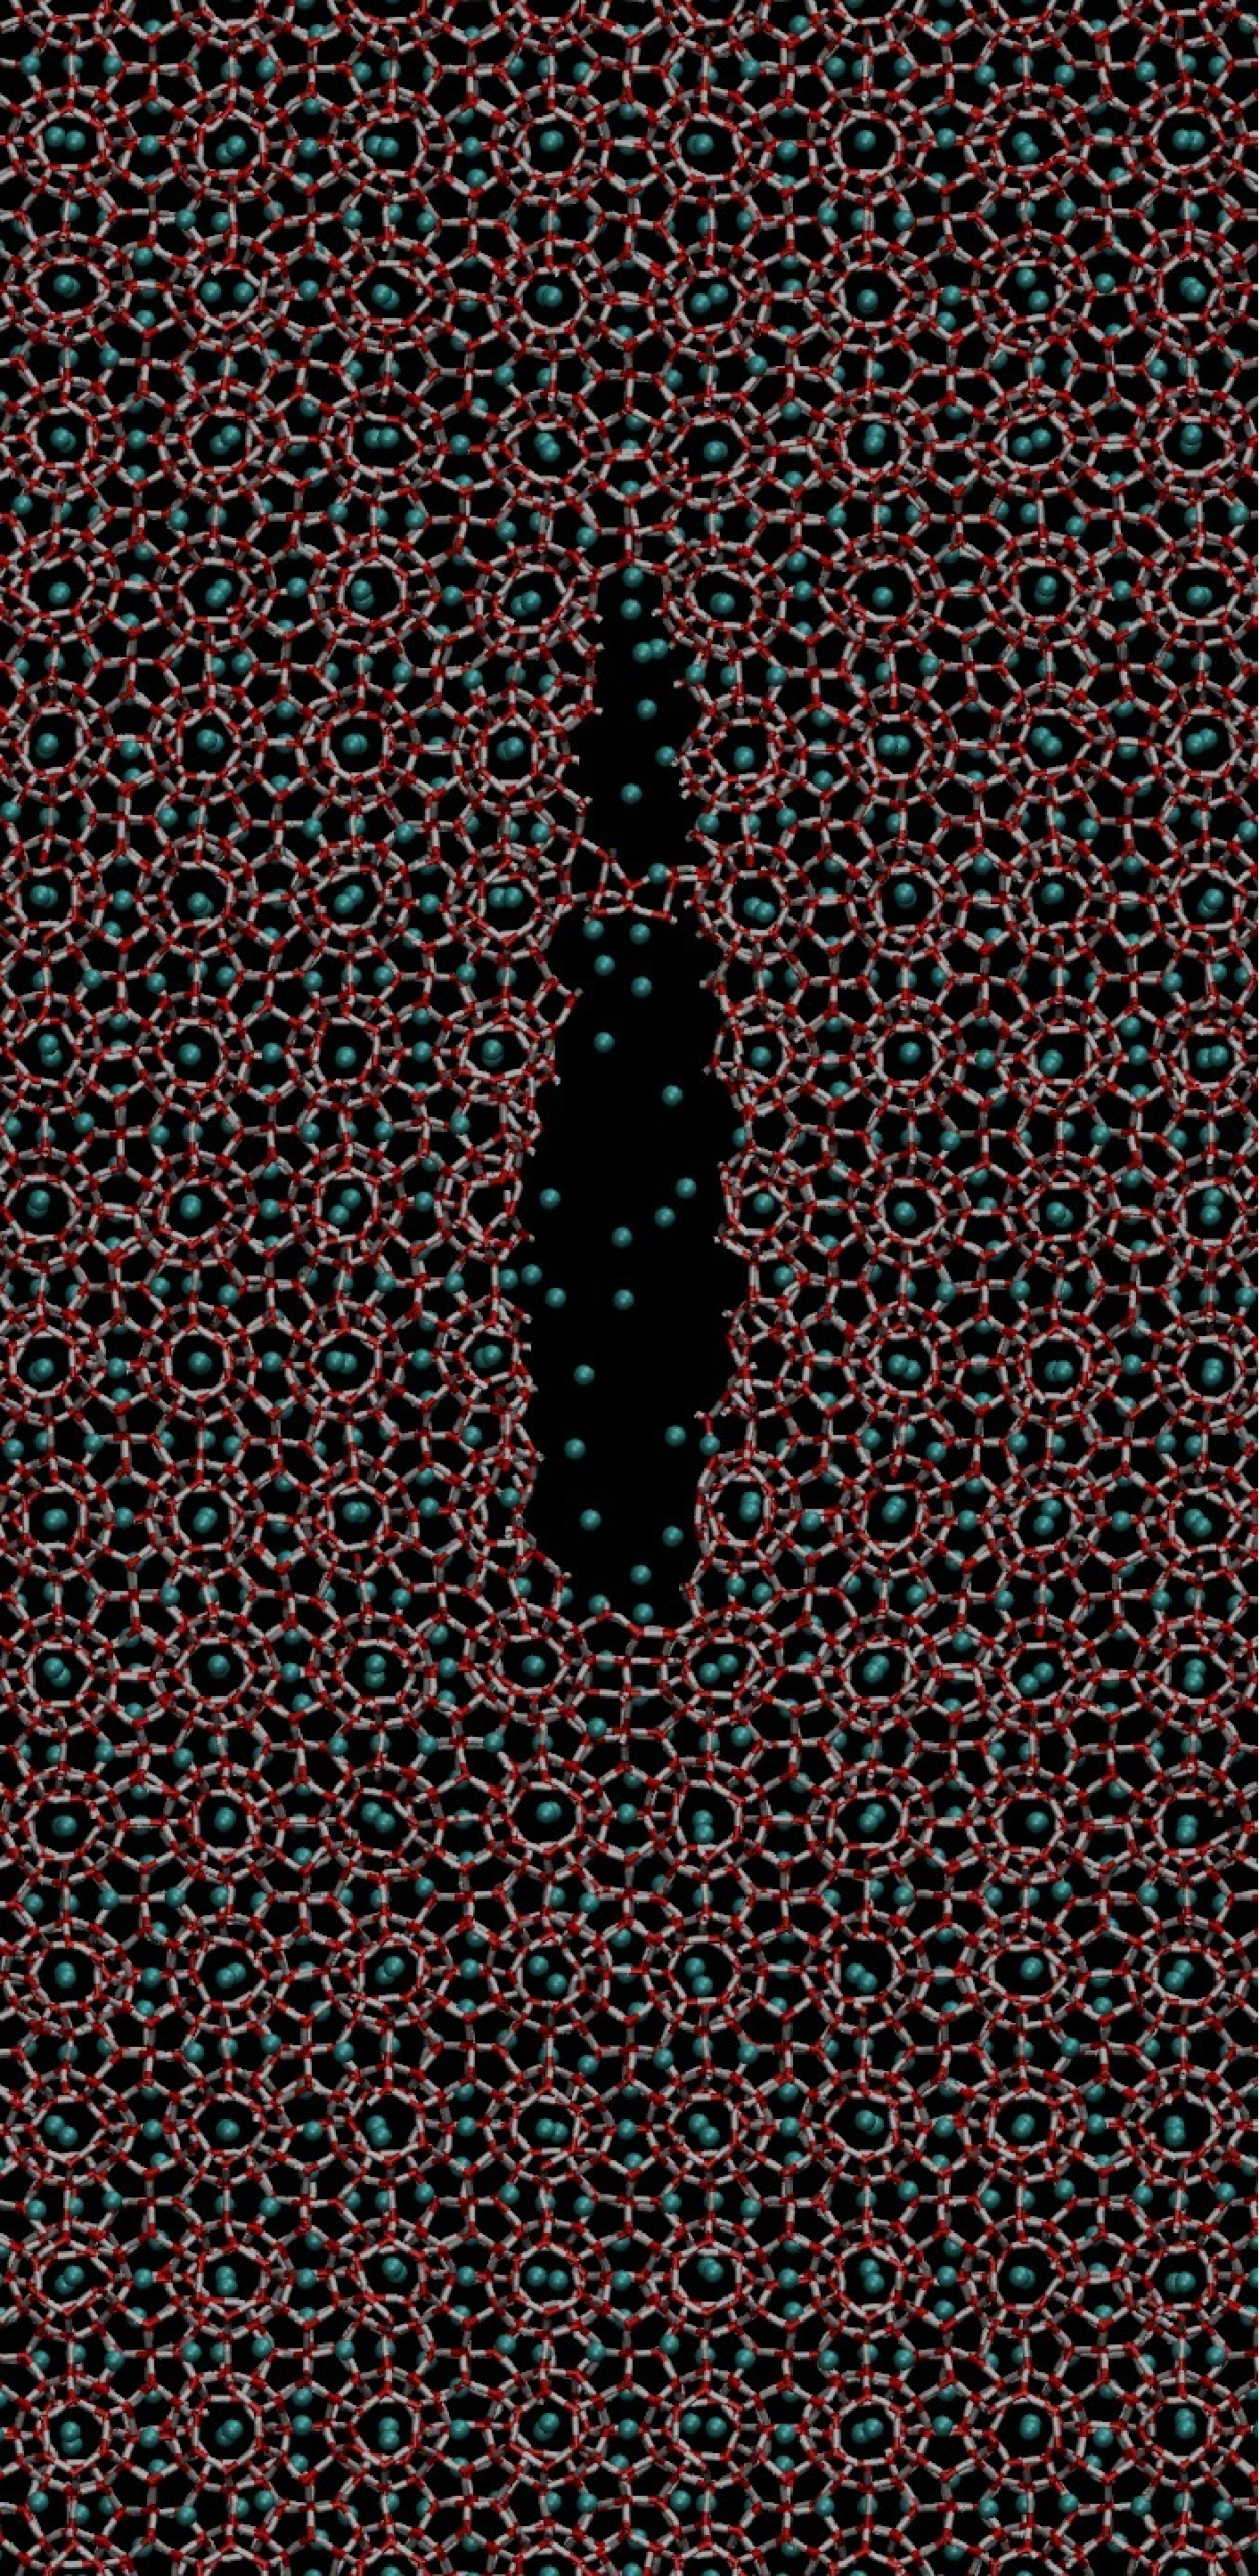
\includegraphics[width=\textwidth]{../pictures/snapshots_cavity_crack/at_555ps.pdf}}
\end{minipage}
\begin{minipage}[b]{0.19\linewidth}
\subcaptionbox{$t=\SI{561}{\pico\second}$}{
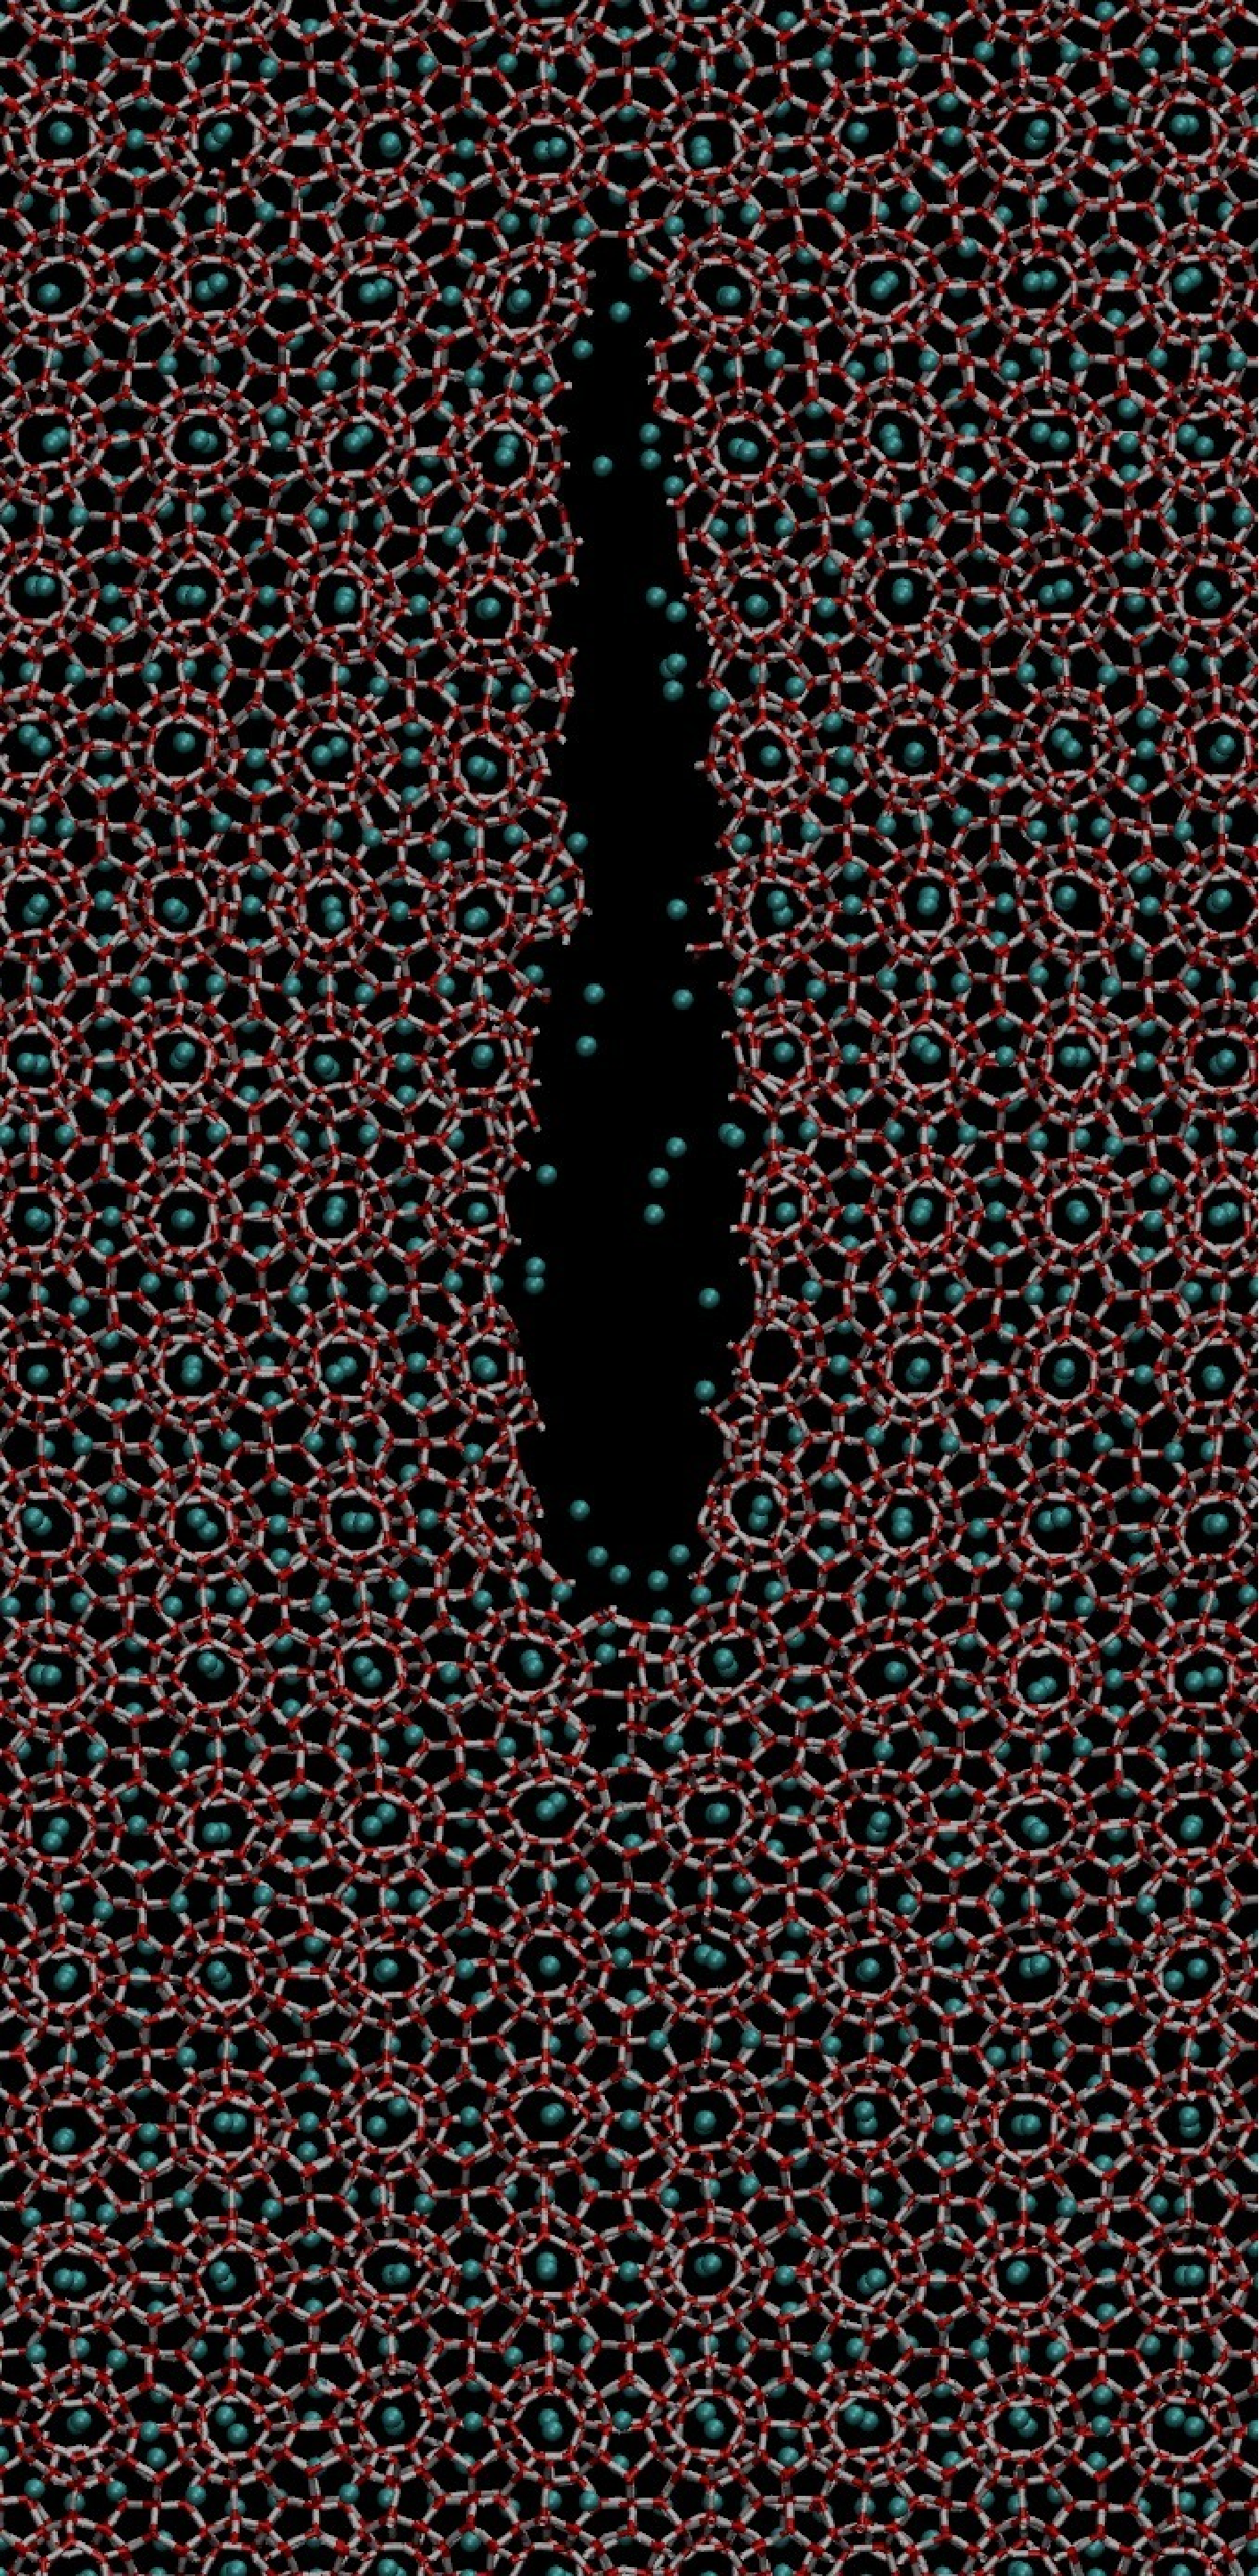
\includegraphics[width=\textwidth]{../pictures/snapshots_cavity_crack/at_561ps.pdf}}
\end{minipage}
\begin{minipage}[b]{0.19\linewidth}
\subcaptionbox{$t=\SI{582}{\pico\second}$}{
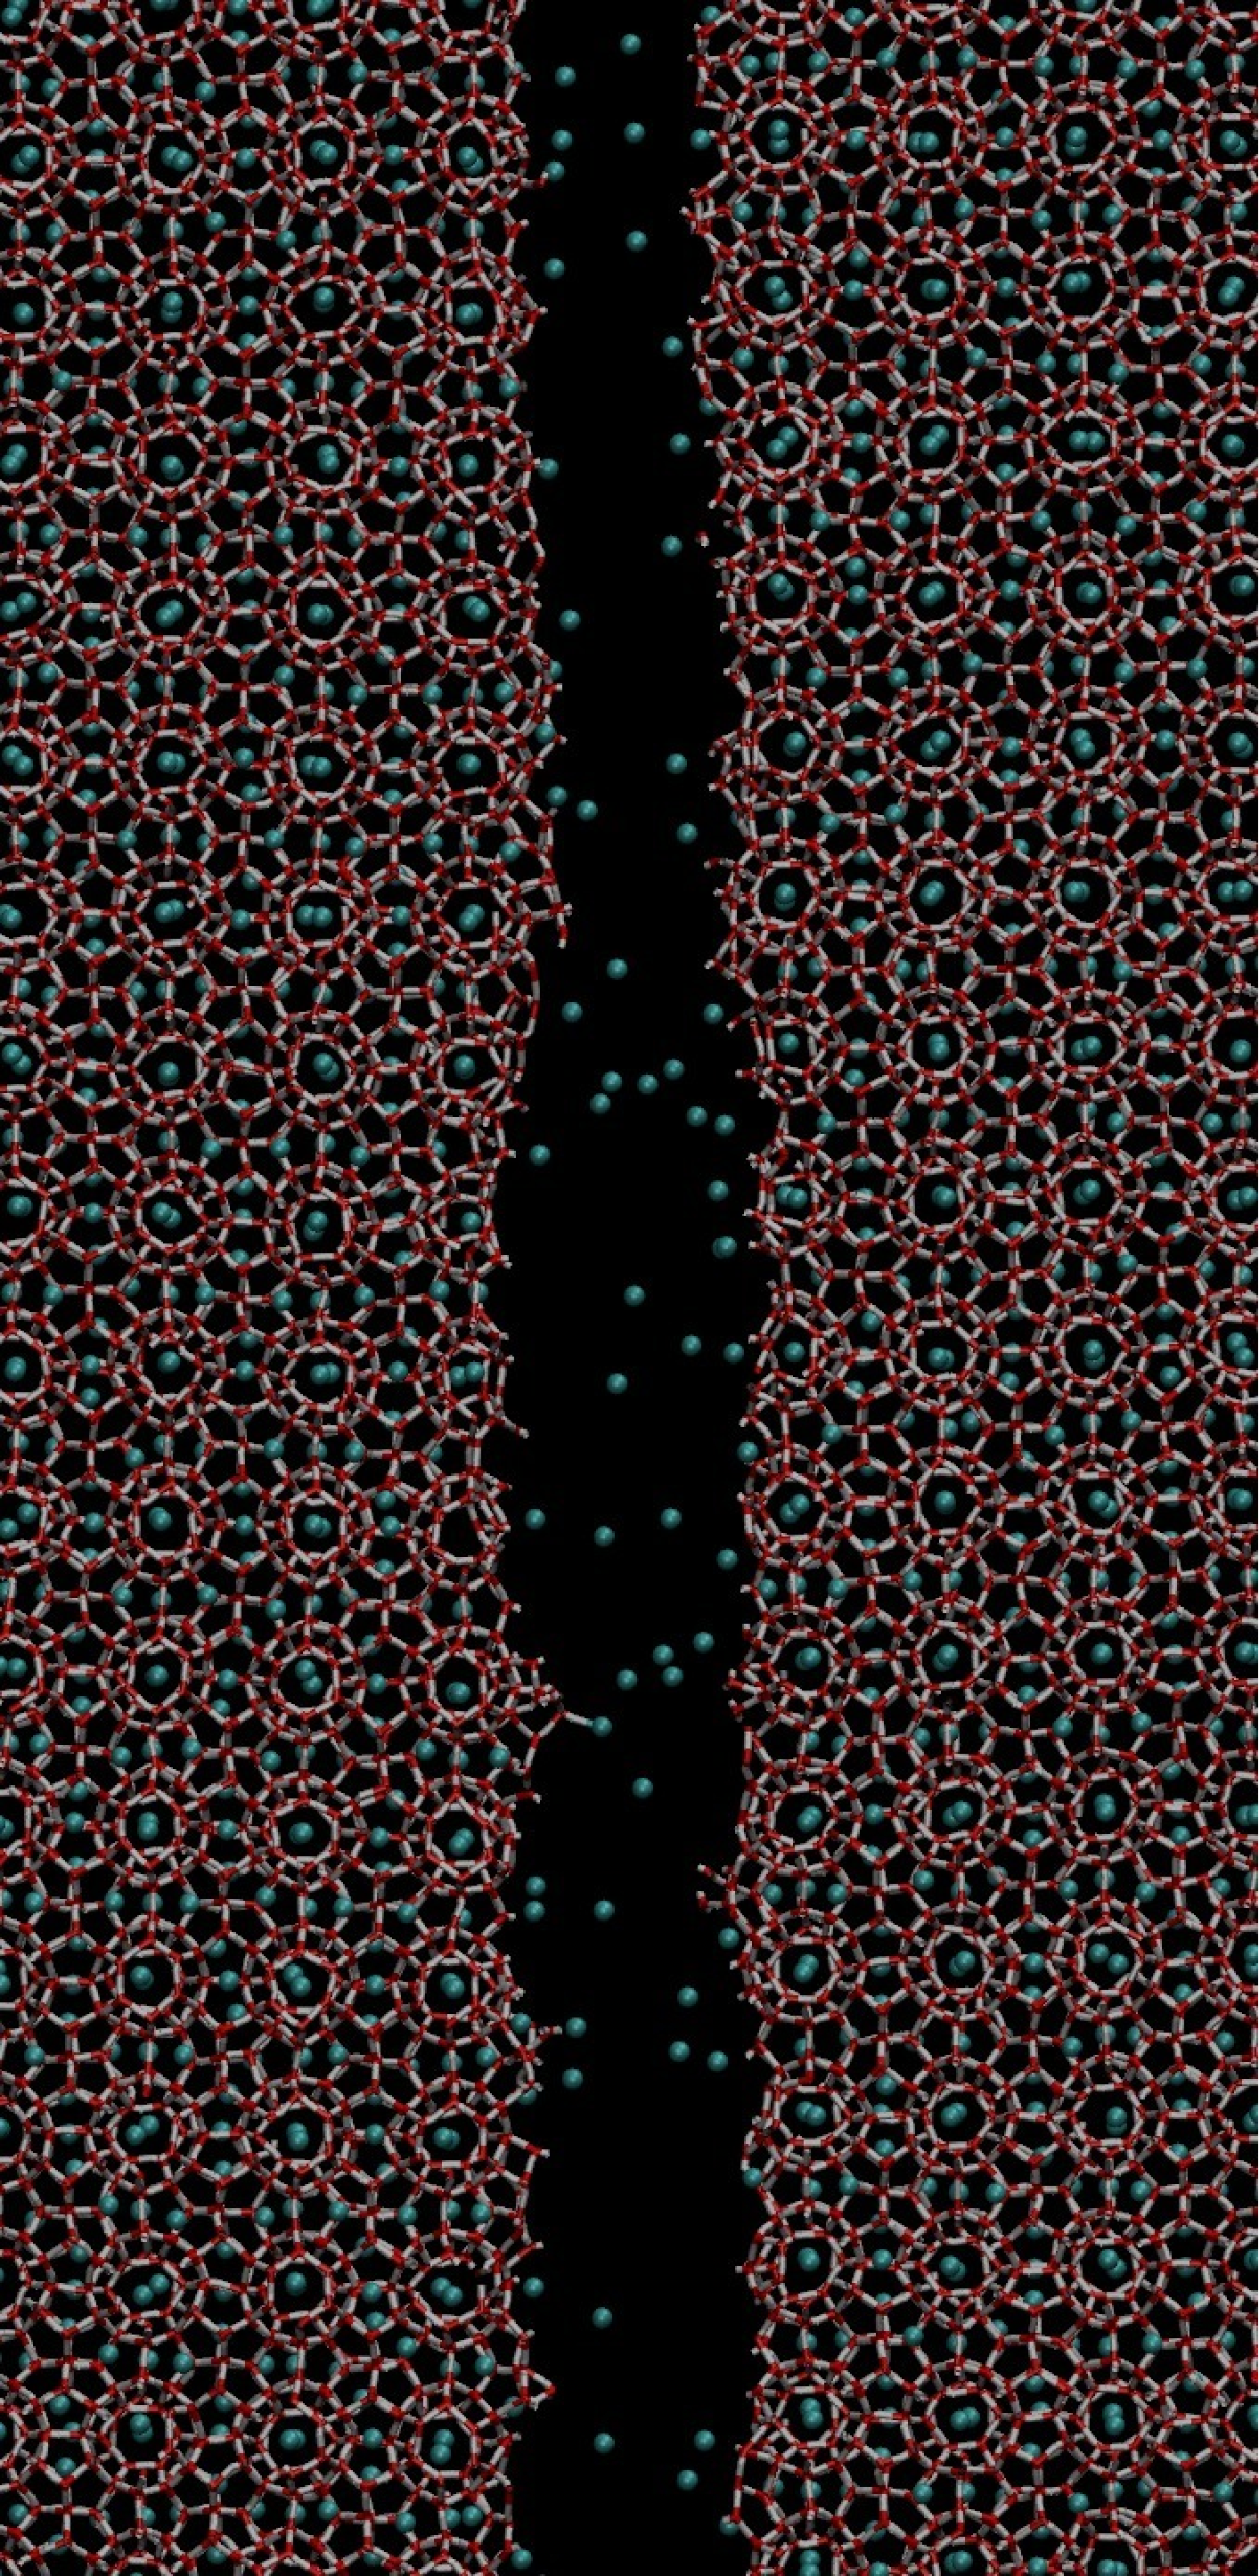
\includegraphics[width=\textwidth]{../pictures/snapshots_cavity_crack/at_582ps.pdf}}
\end{minipage}
\caption{Development of a cavity in front of the crack and then propagation of the crack.}
\label{fig:cavity_crack}
\end{figure}


\subsection{Arising questions}
Several question arise as a result of the proof-of-concept runs:
\begin{itemize}
\item Is the amount of methane that is freed during fracture propagation always the same?
\item Is there a relationship between the waiting time from straining ends till rupture starts and the slope of the potential energy curve?
\item Is the slowly decreasing potential energy of long waiting-time events important, and can it be related to the waiting time?
\item What is the fracture toughness for long (infinite) waiting times, and is it possible to measure? Will the system melt before it fractures?
\item Is the methane in the initial crack important for fracture initiation?
\end{itemize}

There are also several technical problems that can be addressed:
\begin{itemize}
\item What is the effect of the thermostat damping time on fracture properties?
\item Is the strain rate important? Does the time it takes to strain the system compete with the waiting time until fracture?
\end{itemize}

Each of these questions will require substantial efforts to be answered, and I will only have time to address a few of them. In the sections to come, I focus on the crack initiation, and the amount of free methane before, during and after crack propagation. I will essentially ignore the technical issues for now. If I find something interesting, the technical issues will of course be part of the verification -- but I cannot justify the computational cost of such verifications before I have found anything interesting, surprising or counterintuitive that needs thorough verification.

%%%%%%%%%%%%%%%%%%%%%%%%%%%%%%%%%%%%%%%%%%%%%%%%%%%%%%%%%%%%%%%%%%%%%%%%%%%%%%%%%%%%%%%%%%%%%%%%%
\section{Energy considerations -- the thermodynamics of expanding the simulation box}
%%%%%%%%%%%%%%%%%%%%%%%%%%%%%%%%%%%%%%%%%%%%%%%%%%%%%%%%%%%%%%%%%%%%%%%%%%%%%%%%%%%%%%%%%%%%%%%%%
\label{sec:energy_considerations}
The result that $\mathcal{G}_c > 2\gamma_s$, as was found from the preliminary results was peculiar -- and wrong. In this section, I make an argument for why the potential energy cannot be directly used to calculate the fracture toughness. I am probably not the first person to make this argument, but I have not seen it made explicitly. I have found papers, eg. \citet{Hantal2014}, where the same kind of argument must have been made, either explicitly or implicitly, during the research process. 

In the last section, I only considered the potential energy to estimate the fracture toughness, since fracture mechanics dictates that the fracture toughness should be the amount of potential energy released per projected crack surface area opened. But really, it is the Helmholtz free energy release rate that should be used for fracture toughness calculations -- potential energy in fracture mechanics is not necessarily the same as in molecular dynamics. A more thorough analysis solves the problem of methane hydrates seeming very brittle while having $\mathcal{G}_c > 2\gamma_s$, and the conclusion, which we shall see, is that we actually have $\mathcal{G}_c \approx 2\gamma_s$.

Let us consider expanding the simulation box along the x-axis. This corresponds to performing work on the system:
%
\begin{equation}
	W = \int_{t(L_x = L_x^0)}^{t(L_x^0 + \Delta x)} \int_{yz} \sigma_{xx} (t, y, z) \ \dd z \dd y \dd x
\end{equation}
%
If the system is in equilibrium, then:
\begin{equation}
\int_{yz} \sigma_{xx} (t, y, z) \ \dd z \dd y = L_yL_z\Sigma_{xx}(t)	
\end{equation}
Where $\Sigma_{xx}$ is an element of $\uuline \Sigma$, which is the mean stress tensor for particles in the system. The work on the system can then be written:

\begin{equation}
	W = L_y L_z \int_{t(L_x = L_x^0)}^{t(L_x^0 + \Delta x)} \Sigma_{xx}(t) \ \dd x
	\label{eq:work_expansion}
\end{equation}
This expression can be extracted from a molecular dynamics simulation, since both the per-atom stress and the stress of the entire simulation box is readily available.
In the canonical ensemble (NVT), the change of internal energy will be:
\begin{equation}
	\Delta U = W + T\Delta S
\end{equation}
When expanding the system, the entropy per temperature will increase, as more microstates become available. This has to be compensated by adding heat. In molecular dynamics, the thermostat effectively adds energy as entropy during simulation box expansion. Furthermore, this energy cannot increase the kinetic energy, since N and T are kept fixed, so all the added heat must be absorbed as \emph{potential} energy. This means that expanding the simulation box adds a lot of potential energy to the system, both directly through mechanical work, and indirectly through heat. Storage of the mechanical work is in line with the intuition -- particles are positioned higher in each others potentials. The heat absorption is more subtle: The system creates more available microstates when it expands homogeneously at a constant temperature. These microstates do only exist because of the strained state of the system, and will disappear if the strain disappears, for example during fracture. The entropy energy is not available for mechanical work. This is why Helmholtz free energy should be considered:

\begin{equation}
	F = U - TS
\end{equation}
%
This is exactly the energy available for mechanical work. The reason for this tedious discussion of expanding a box is that Helmholtz free energy is not directly available from molecular dynamics simulations. The change in Helmholtz free energy must be explicitly calculated by integrating the stress tensor of the system with incremental box deformations. When analyzing fracture, it is tempting to use the change in total energy or potential energy to calculate the fracture toughness. But this would be wrong -- the fracture toughness should be calculated using the available mechanical energy. The energy release rate is the amount of Helmholtz free energy needed to create the projected crack surface area, not the change in potential energy or total energy of the system during fracture. This distinction is not easy to see when reading fracture mechanics, as fracture mechanics usually deal with elastic bodies with no temperature, but it is crucial when studying fracture in molecular dynamics.

When the crack propagates, the stress in the methane hydrate is released, and the system consists of a piece of methane hydrate, and some free gas in between. The entropy of this system is unknown, which means that calculating the surface energy becomes complicated. I have not gone further in how to calculate the surface energy, and assume that the entropic energy contribution by the free methane is small compared to the mechanical energy contributed by the crack surface opening. I find some support to this assumption, in the fact that the final potential energy in the proof-of-concept runs with different final strains were seemingly equal.


\citet{Hantal2014} proposes to calculate the critical energy release rate with the following formula (This method was used for illite with ClayFF and ReaxFF):
\begin{equation}
	\mathcal{G}_c = V \frac{\int_0^{E_{\text{final}}}\uuline{\Sigma}(E) : \dd \uuline{E}}{\int_0^{E_{\text{final}}} \dd A_{crack}}
	\label{eq:hantal_critical_energy_release_rate}
\end{equation}
%
This is in principle sufficient to determine the critical energy release rate for any mode of loading
For expansion of the simulation box along the x-axis, the strain integral (nominator) is equivalent to equation \ref{eq:work_expansion}. The area integral (denominator) is just the crack area in time, which can be estimated using the crack tracer I described in chapter \ref{ch:tools}. For reference, \citet{Hantal2014} also used a variation of the crack tracer algorithm that I have chosen to use.

Using equation \ref{eq:hantal_critical_energy_release_rate} to measure the strain energy, I can recalculate the fracture toughness. I run a series of new simulations to be able to pinpoint the strain level at which the hydrate fails. Figure \ref{fig:pot_strain_eng_l1} shows the potential energy \emph{and} the strain energy from a simulation where the strain before crack propagation was 0.048. It is clear from the figure that the entropic energy contribution (which is supplied by the thermostat) is larger than the strain energy, which means the total potential energy gives a bad estimate of the free energy, and ultimately, gives a bad estimate of the fracture toughness. This particular simulation is chosen because it is the simulation with the lowest required strain level to support a crack in a series of simulations with a strain increment of 0.001. The strain energy in this simulation is \SI{0.01455}{\femto\joule}. The cross-sectional area of the simulation box is $\SI{12.04}{\angstrom} \times \SI{288.8}{\angstrom}$, so my current best estimate of the critical energy release rate is $\mathcal{G}_c = \SI{0.42}{\joule\per\meter\squared}$. This corresponds to a fracture toughness of $K_{Ic} = 0.060$ MPam$^\frac{1}{2}$.



\begin{figure}
\centering
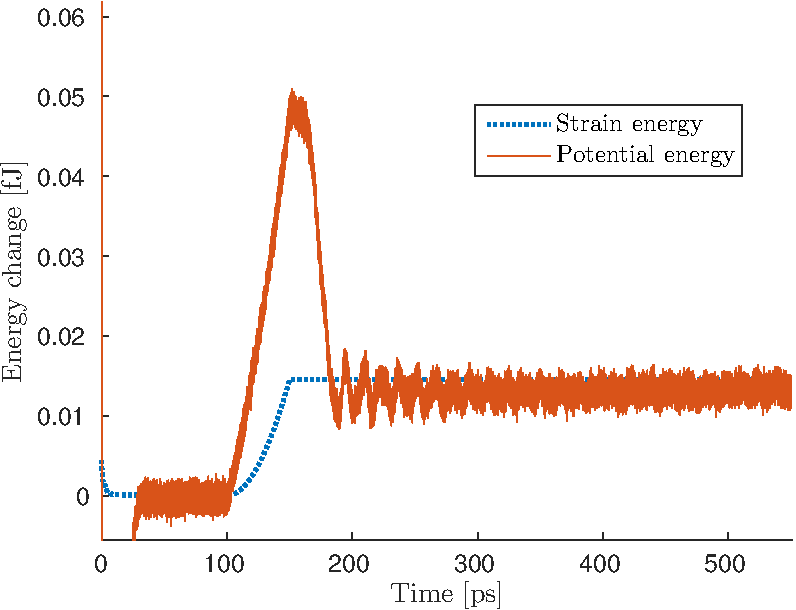
\includegraphics[width=12cm]{../figures/thesis/pot_strain_eng_24_24_1.pdf}
\caption{Potential energy and strain energy from a simulation where the strain before crack propagation is 0.048. The strain energy difference from before to after straining is \SI{0.01455}{\femto\joule}. It is clear from this figure that the entropic energy introduced during straining is higher than the strain energy.}
\label{fig:pot_strain_eng_l1}
\end{figure} 

%%%%%%%%%%%%%%%%%%%%%%%%%%%%%%%%%%%%%%%%%%%%%%%%%%%%%
\section{Large simulations of fracture}
%%%%%%%%%%%%%%%%%%%%%%%%%%%%%%%%%%%%%%%%%%%%%%%%%%%%%
Larger simulations allow for statistically more robust results. During crack initiation in the previous simulations, only a few particles near the crack tip ended up being essential to the crack initiation. Even though the periodic boundary condition allows for the crack to be thought of as infinitely deep, the low number of particles makes the crack initiation vulnerable to statistical fluctuations. With thicker systems, more particles reside in the region near the crack tip, resulting in better statistics. An obvious drawback of larger simulations, is the added computational cost. Also, the amounts of data increase drastically if per-particle properties are to be stored. My approach has been to post-process trajectory data from simulations, which means I have had to deal with large amounts of data. This has actually been a challenge when working with large simulations, and has required close attention to efficiency in file handling, both to reduce the CPU-time of analyses, and to keep the memory demands on an acceptable level. Also, the amount of data that can be output is limited. Outputting all positions and velocities in a simulation of $10^6$ particles require around \SI{50}{\mega\byte} per timestep. That becomes \SI{50}{\tera\byte\per\nano\second} for a timestep of \SI{1}{\femto\second}. 
\label{sec:complete_analysis_single_simulation}

\subsection{Complete analysis of a single simulation}
In the following, I use the analysis tools that were presented in the tools section to analyze \emph{one} simulation. This simulation will be referred to as the \emph{full-analysis simulation}. The analyzes here will be representative of how data is obtained when showing up in later results where data from several simulations are used together to say something more general.

\begin{figure}
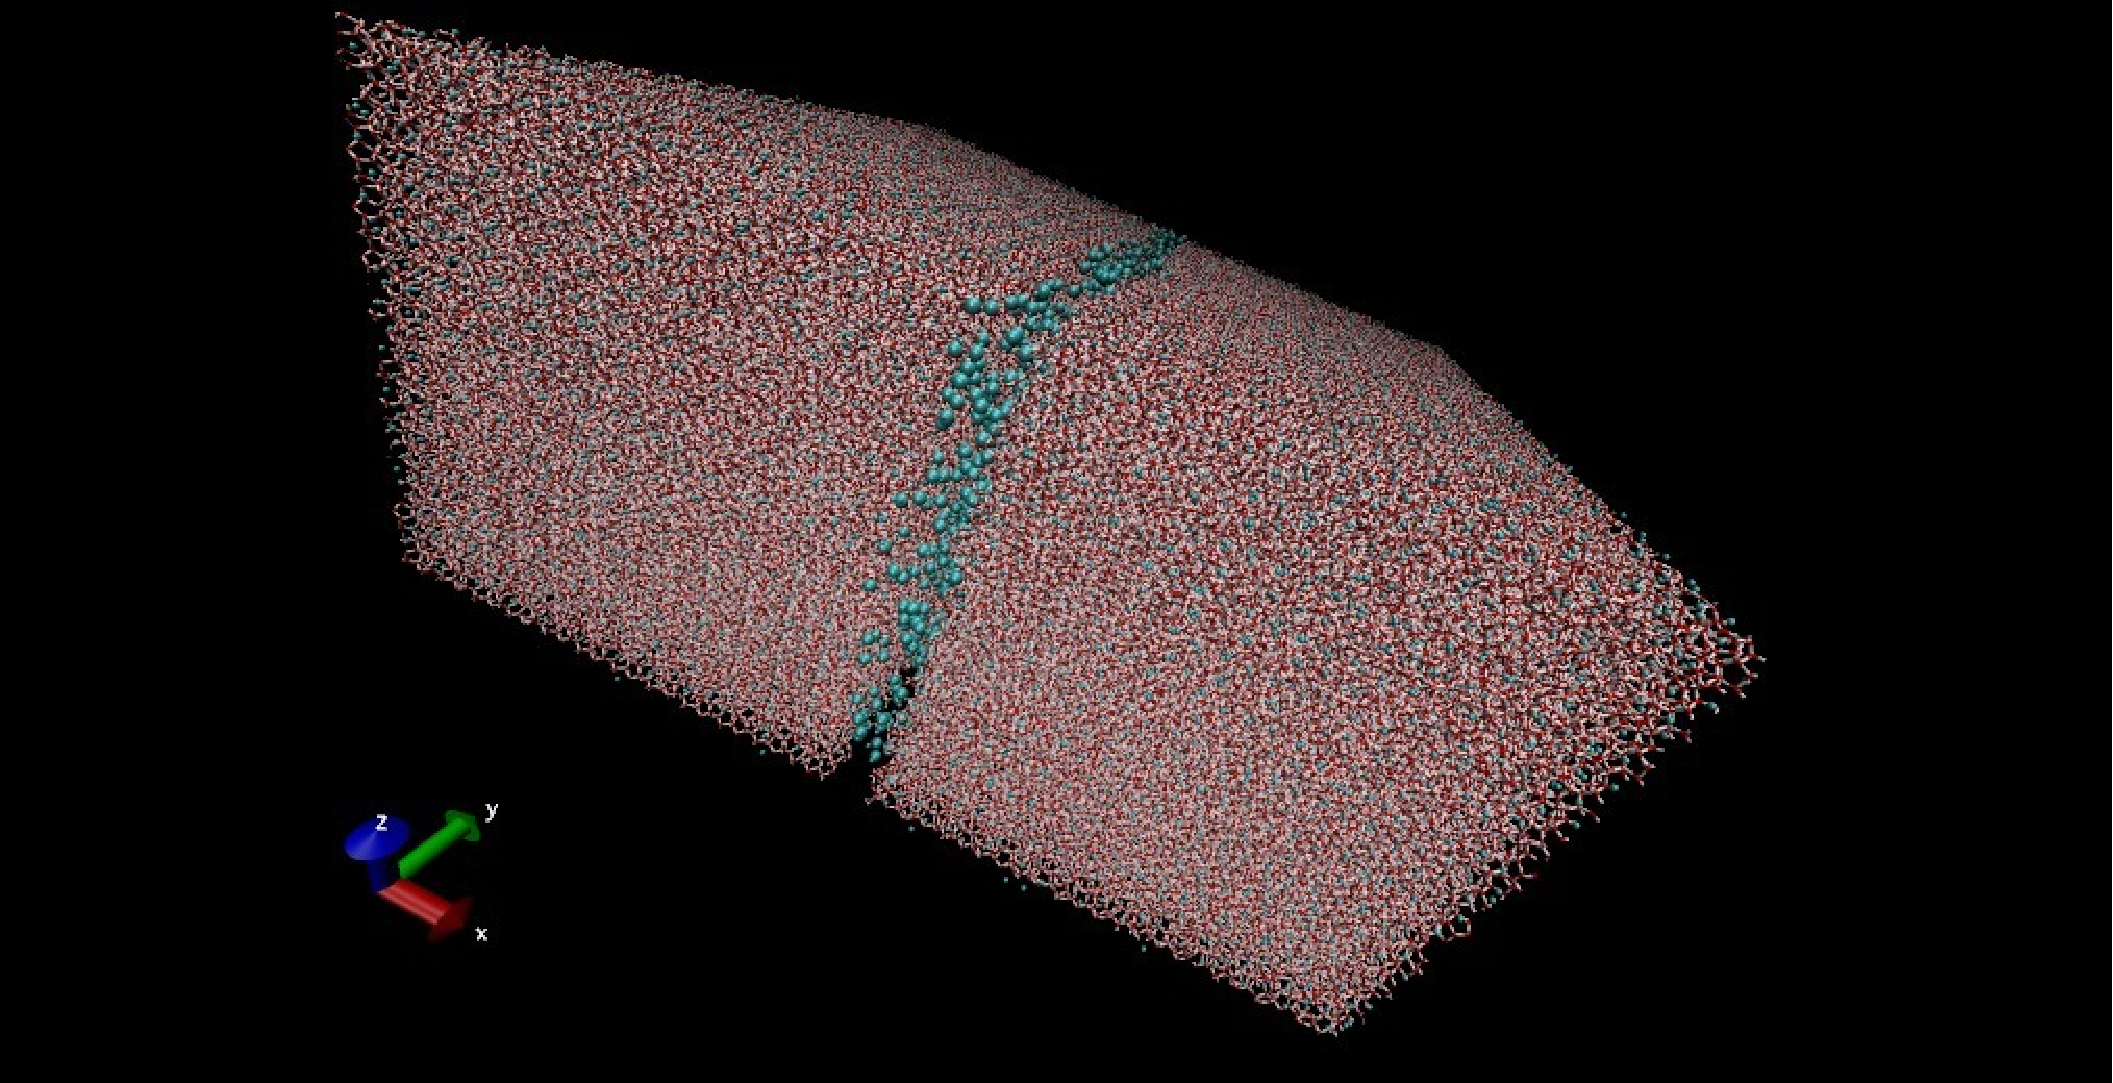
\includegraphics[width=\textwidth]{../pictures/system_1048.pdf}
\caption{Perspective image of a representative state after fracture in a $24\times 24 \times 12$ sI unit cell simulation. The biggest green spheres are methane molecules that are considered free to move (not enclathrated). Smaller green spheres (barely visible) are enclathrated methane molecules. Water molecules are drawn as hydrogen bonds.}
\label{fig:system_1048}
\end{figure}

\begin{framed} 
\textbf{Simulation details:} A system consisting of $24 \times 24\times 12$ sI unit cells is prepared. First, an elliptical hole in the $xy$-plane spanning the whole z-direction is carved out as described in section \ref{subsec:reg_eprism}. The system is then allowed to equilibrate with an anisotropic NPT thermo-barostat for \SI{100}{\pico\second}, with ambient barostat pressure (\SI{101325}{\pascal}). The system is then integrated NVT, but subjected to a constant strain rate taking it to a strain level of $\epsilon_{xx} = 0.048$ after \SI{50}{\pico\second}. Then straining is stopped, and the system is left NVT for \SI{350}{\pico\second}. The damping time of the thermostat and barostat during the whole simulations is $t_{damp} = \SI{1}{\ps}$. Additionally, a drag coefficient of $1.0$ (as described in the LAMMPS documentation) is added, as this is recommended to damp oscillations in solids. The thermostat temperature is set to \SI{260}{\kelvin}.
\end{framed}

For illustrative purposes, figure \ref{fig:system_1048} shows what the system looks like in perspective. The other pictures are rendered with an orthographic projection, so the system will look two-dimensional. 

Figure \ref{fig:crack_evolution} shows the evolution of the crack in time, to give an idea of what the system looks like during fracture. 

Figure \ref{fig:energy_1048} shows the potential energy, the kinetic energy and the strain energy for the whole simulation. It shows that a strain of 0.048 is only a bit more than what is needed if the criterion for a crack to propagate is $\mathcal{G}_c = 2\gamma_s$. This means the system shows brittle behavior in this particular simulation. The kinetic energy slightly increases, which means the temperature increases during fracture. This is because the release of heat is faster than what can be absorbed by the thermostat. The temperature is not indicated in the figure, but the temperature change is only by a few Kelvin. 

Figure \ref{fig:stressfield_avg_wait_for_crack} shows all components of the stress tensor of the system in space during the period when the system is fully strained, but before propagation starts. It is averaged over the z-direction in space and over \SI{20}{\pico\second} in time to get statistics for a nice picture. The stress field is visually compatible with the analytical solution close to the crack tip for a homogeneous isotropic linear elastic solid. The shear components normal to the $xy$-plane are small, but not negligible That means the plane strain condition is only partially met. Particularly, the amplitude of $\tau_{xz}$ is about $1/5$ of that of $\tau_{xy}$. 


Figure \ref{fig:stressfield_snap_propagation_180} is similar to figure \ref{fig:stressfield_avg_wait_for_crack}, but it now shows the stress field during crack propagation Since tracking the crack requires higher time resolution, the stresses are only averaged over \SI{0.3}{\pico\second}. As expected, the region of high stresses moves along with the crack tip.

Figure \ref{fig:stressfield_timelapse} shows the stress $\sigma_{xx}$ at several points in time before, during and after crack propagation. Here also, the stresses are only averaged over \SI{0.3}{\pico\second}. The top crack is leading the bottom crack with $\sim \SI{10}{\angstrom}$, which is probably coincidental

Figure \ref{fig:crack_area_evolution_1048} shows the measured crack area in time, and its time derivative which estimates the crack tip speed. The maximum crack tip speed is around \SI{1}{\kilo\meter\per\second}. A little bump can be seen in the crack tip speed during crack propagation. This is a feature that always show up in simulations of the same system but with a different strain. My guess is that it is caused by bulk elastic waves triggered by the crack. The crack tip speed is a measure that is likely to be influenced by the strain level before fracture. 

Figure \ref{fig:free_methane} shows the system after fracture with the free methane -- methane that was released as a consequence of the crack -- indicated as big spheres. This figure is explained later, but the data is from this full-analysis simulation.

\begin{figure}
\begin{minipage}[b]{0.5\linewidth}
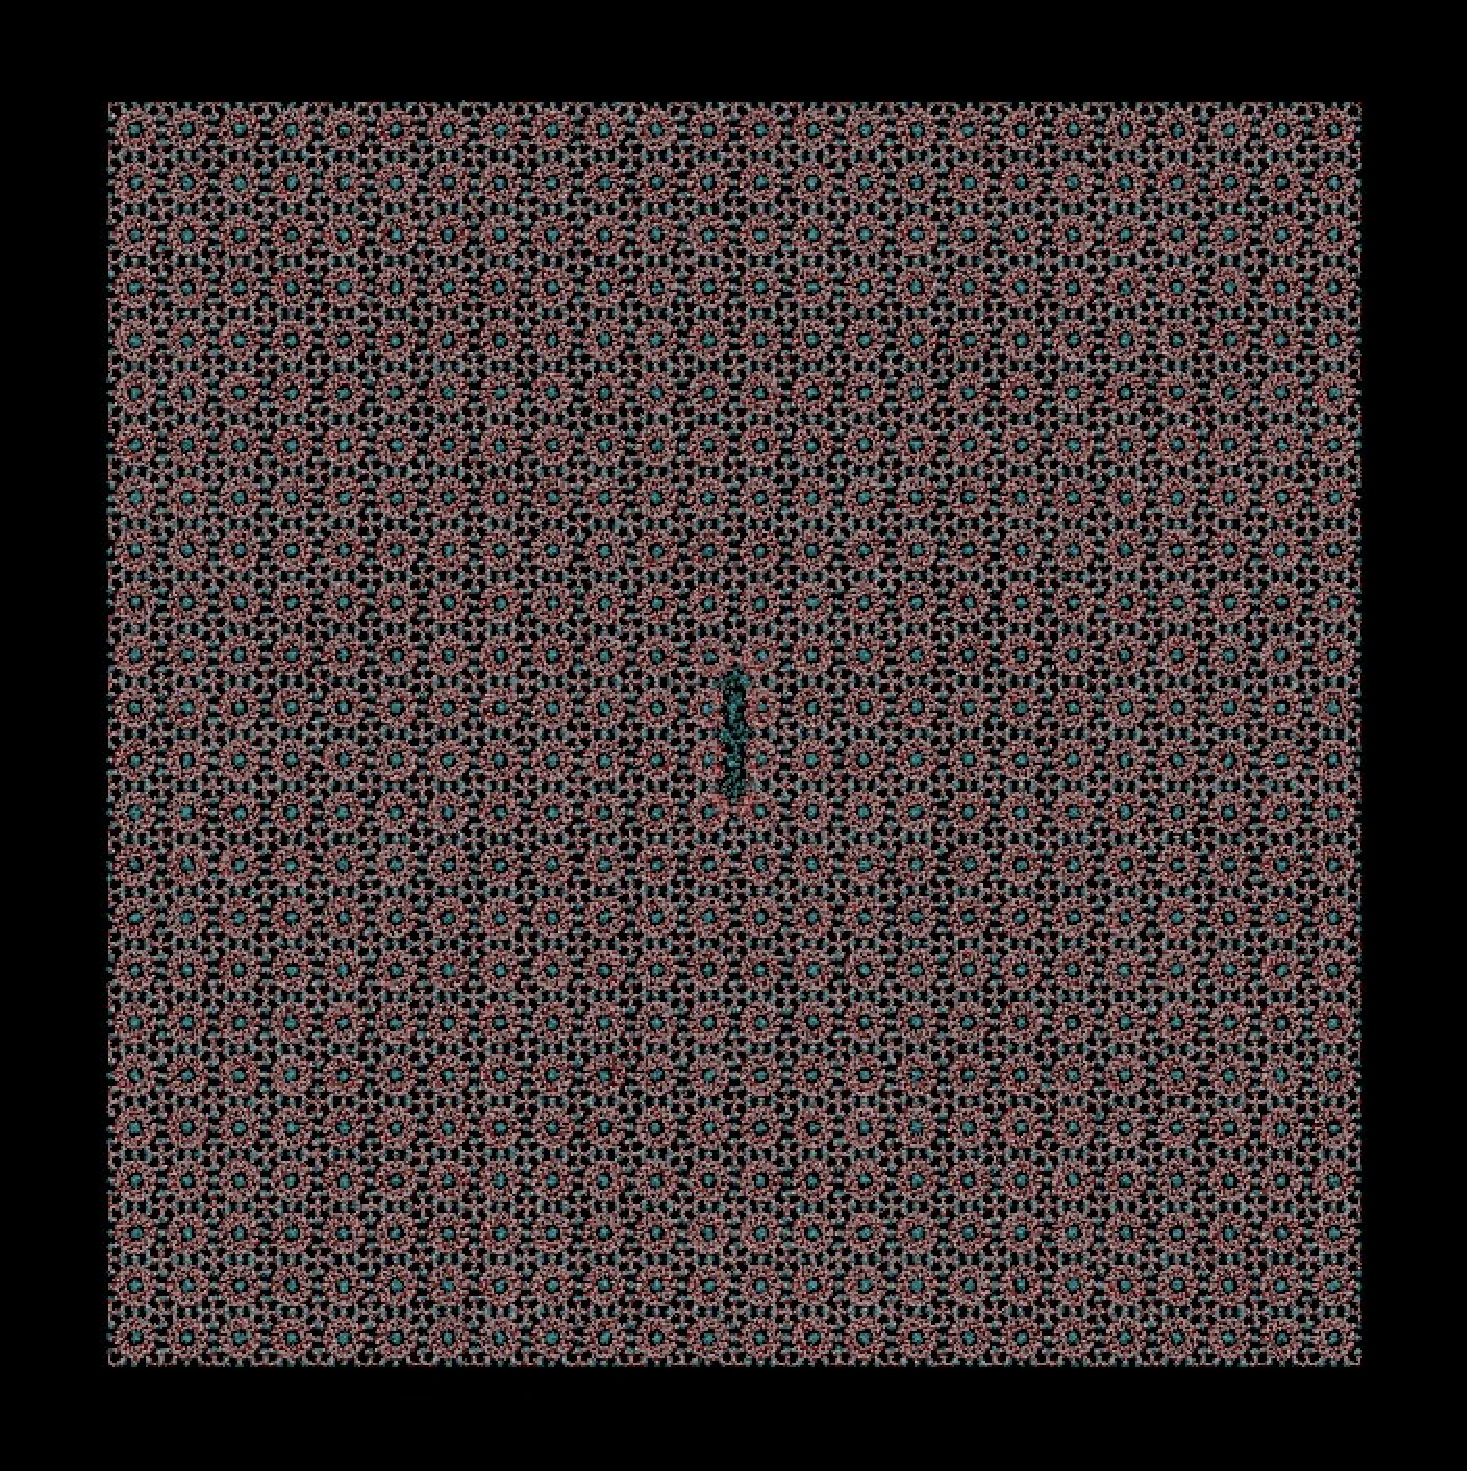
\includegraphics[width=\textwidth]{../snapshots/c_1.pdf}
\end{minipage}
\begin{minipage}[b]{0.5\linewidth}
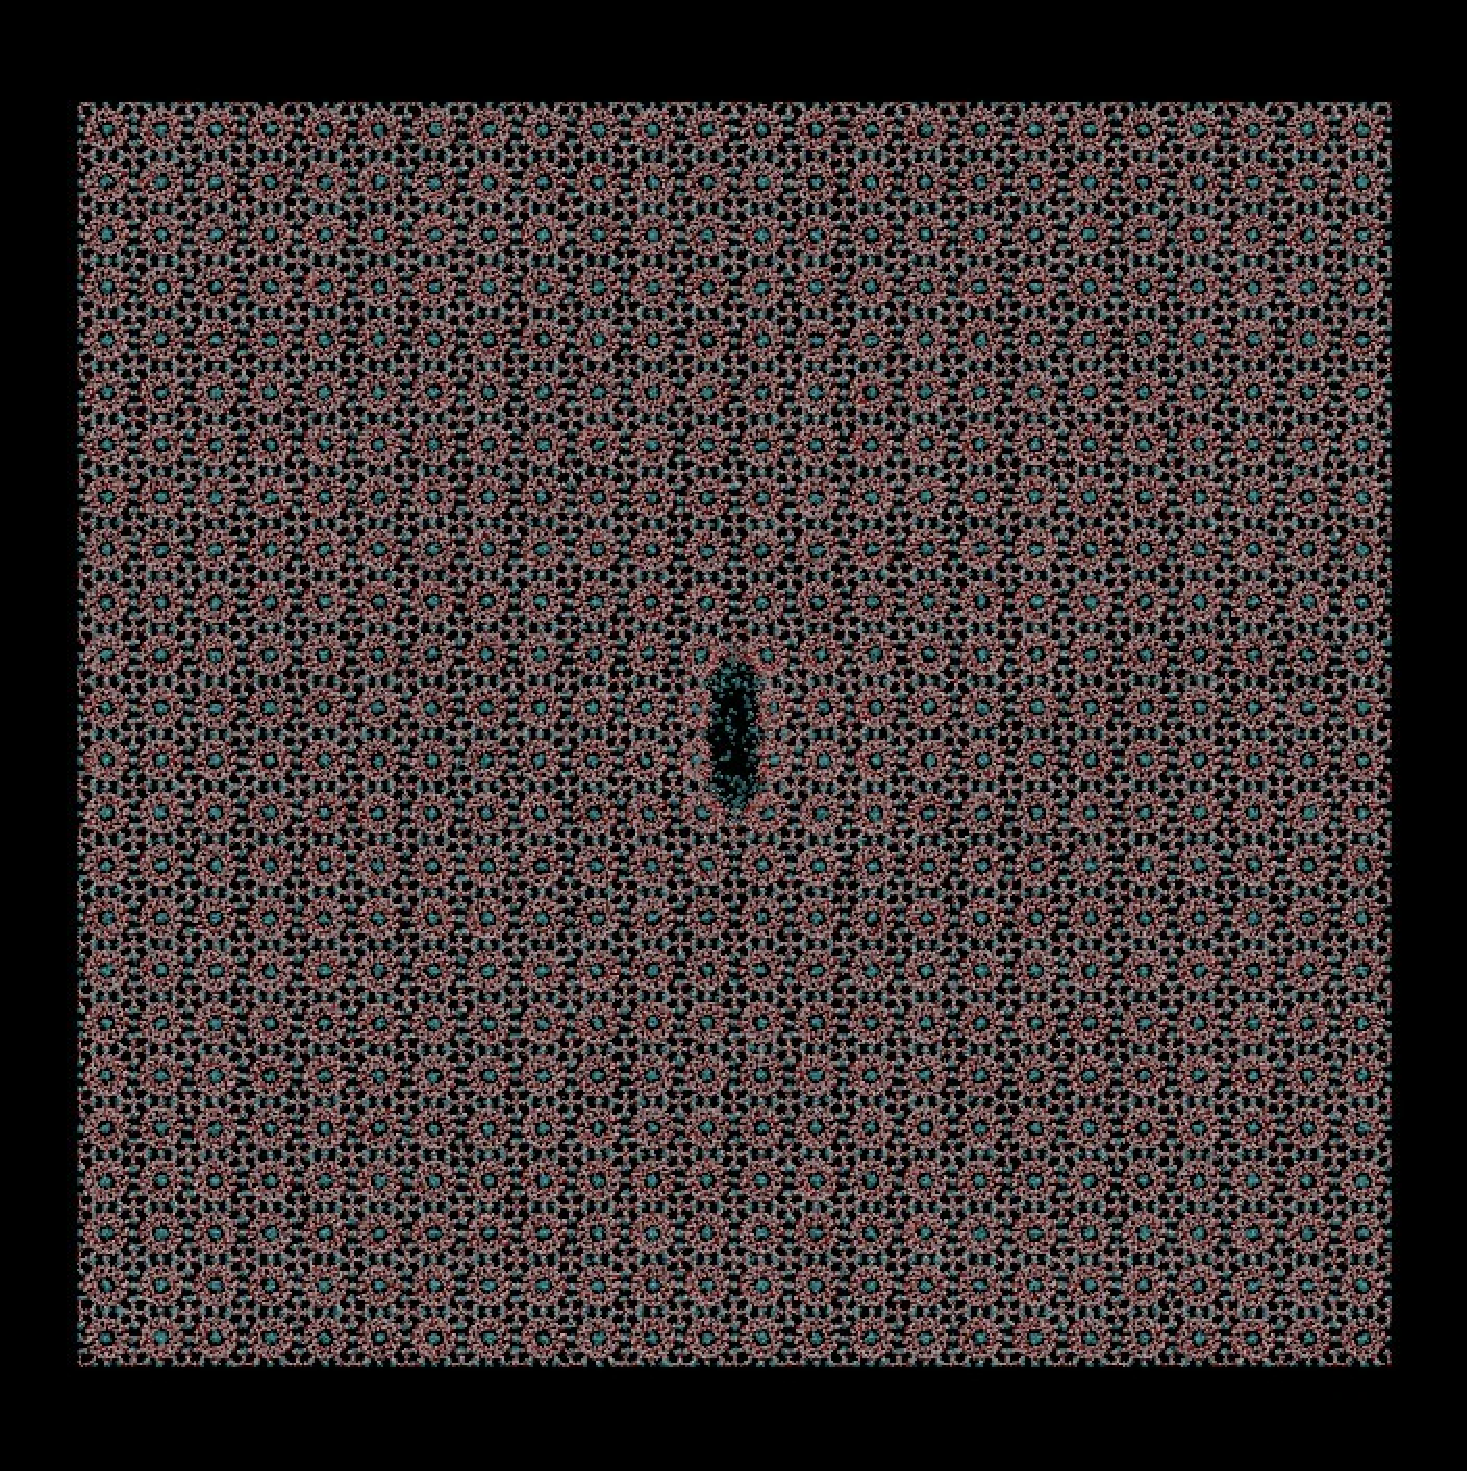
\includegraphics[width=\textwidth]{../snapshots/c_2.pdf}
\end{minipage}
\begin{minipage}[b]{0.5\linewidth}
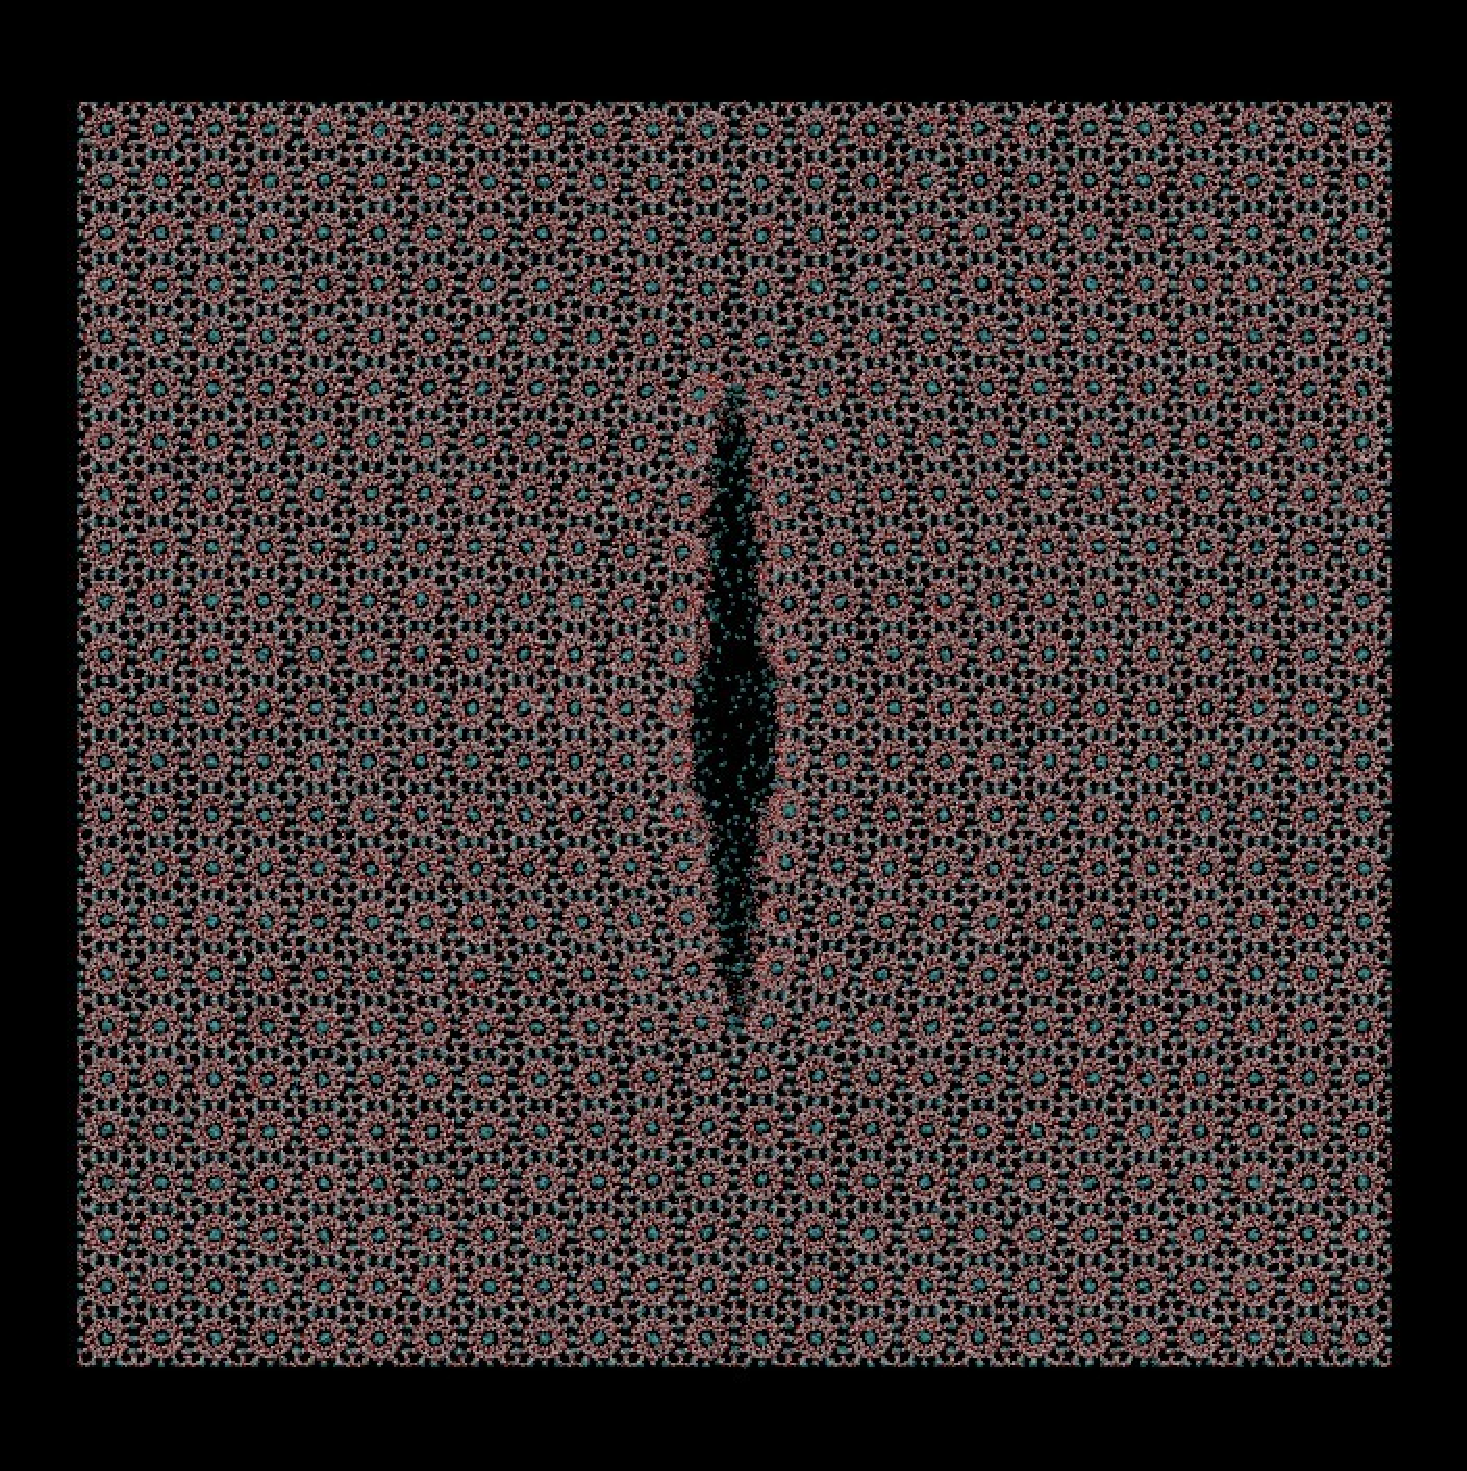
\includegraphics[width=\textwidth]{../snapshots/c_3.pdf}
\end{minipage}
\begin{minipage}[b]{0.5\linewidth}
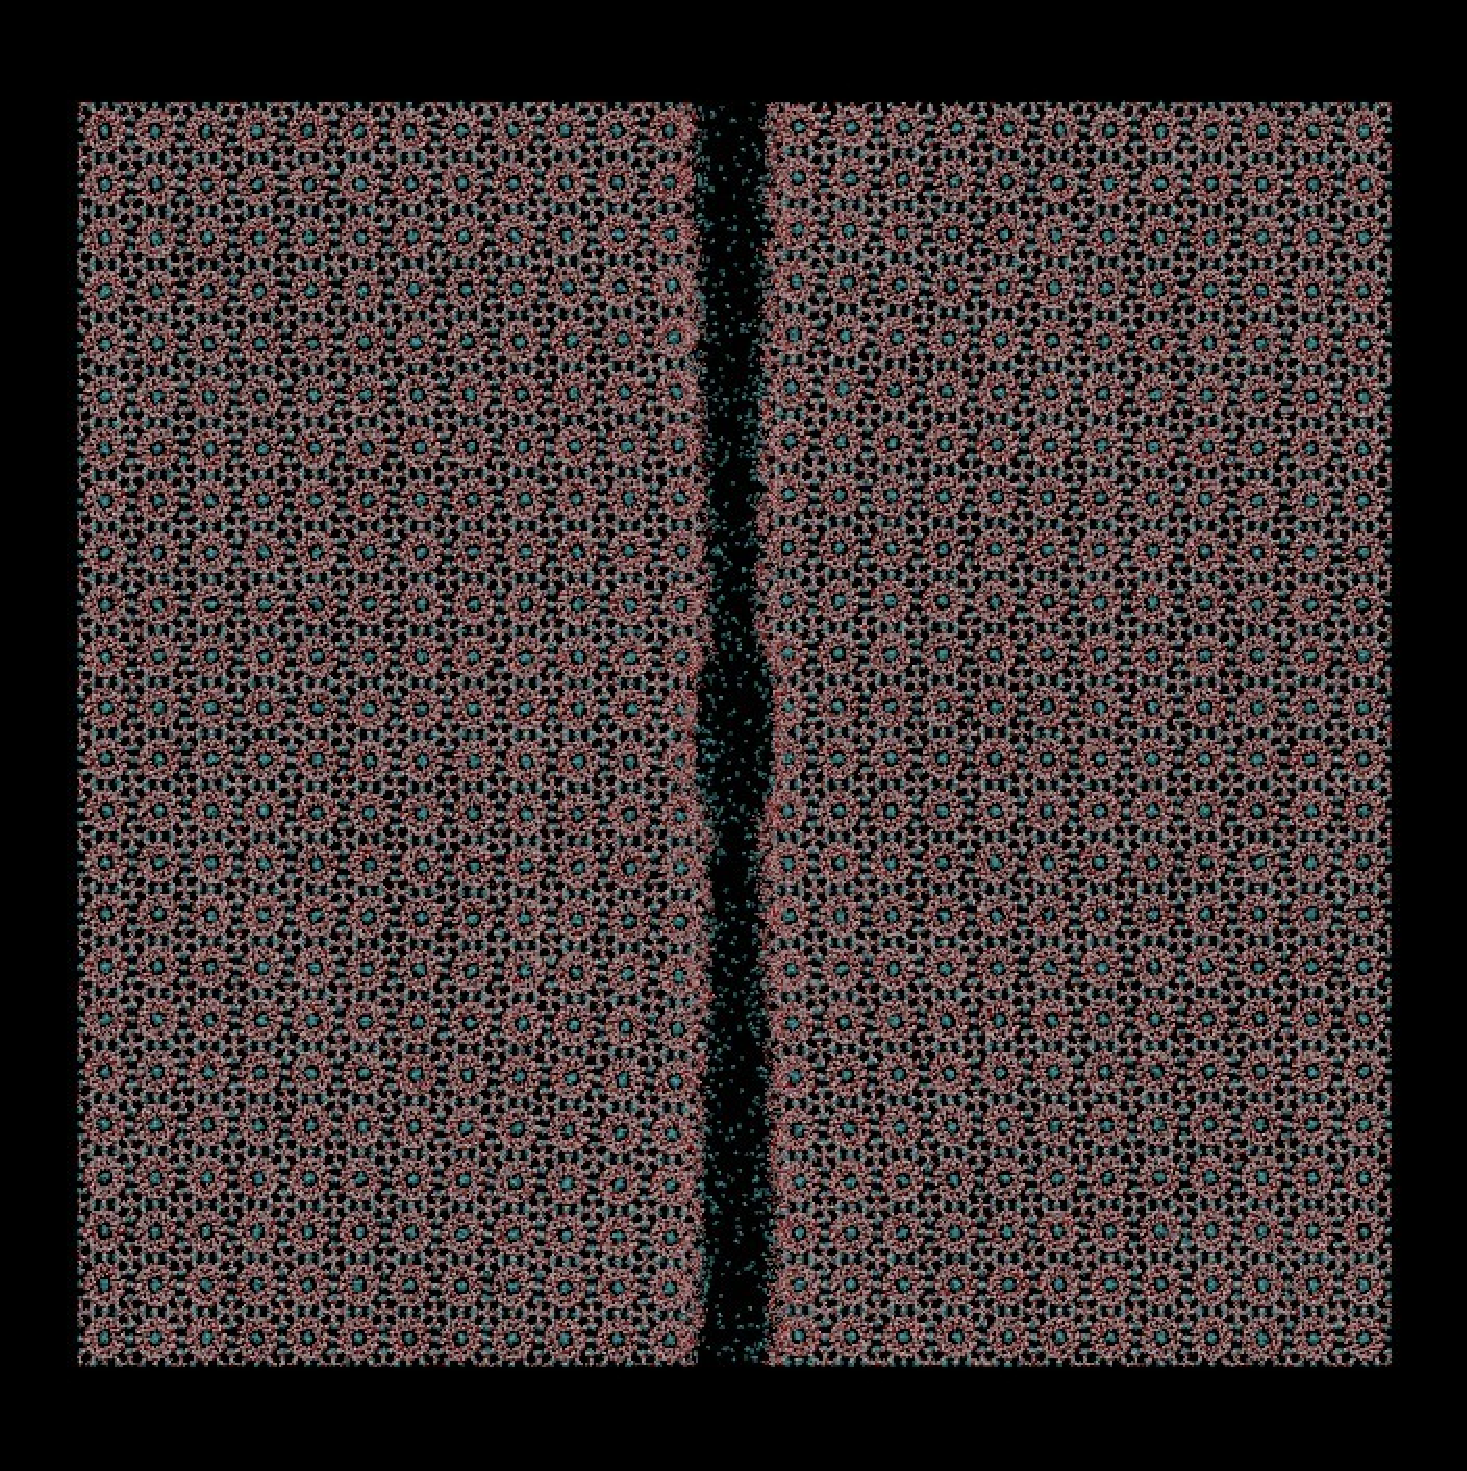
\includegraphics[width=\textwidth]{../snapshots/c_4.pdf}
\end{minipage}
\caption{(upper left) Equilibrated system, \SI{90}{\pico\second}. (upper right) Fully strained system ($\varepsilon_{xx} = 0.048$), \SI{150}{\pico\second}. (lower left) Crack started propagating, \SI{180}{\pico\second}. (lower right) Crack fully propagated after \SI{210}{\pico\second}. The crack is wider near the xz-plane periodic boundary at this point in time due to global oscillations following the crack propagation.}
\label{fig:crack_evolution}
\end{figure}


\begin{figure}
\centering
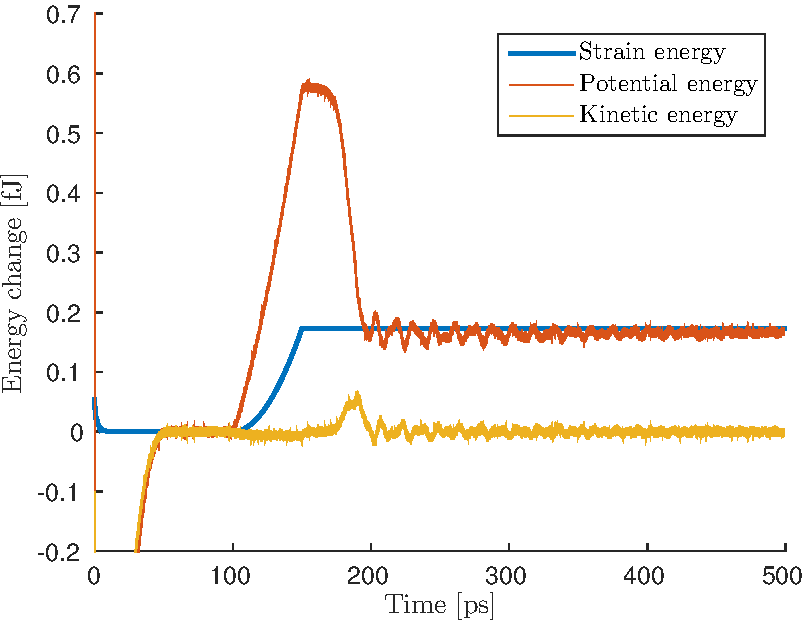
\includegraphics[width=10cm]{../figures/thesis/strain_pot_kin_eng_1048_24_24_12.pdf}
\caption{Strain energy, potential energy and kinetic energy for the whole 0.048 strain simulation. The values are rebased at $t=\SI{100}{\pico\second}$ where straining starts. The kinetic energy corresponds to the temperature, and we see that the temperature slightly drops while the strain increases, and increases during crack propagation. The strain energy imposed on the system is just slightly higher than the energy difference between the unstrained system and the fractured system.}
\label{fig:energy_1048}
\end{figure}

\begin{figure}
\centering
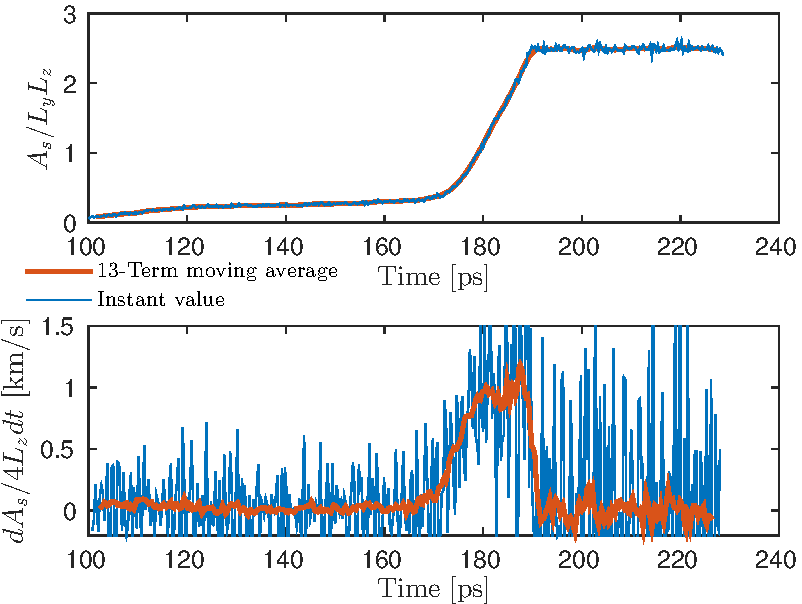
\includegraphics[width=10cm]{../figures/thesis/crack_area_evolution_1048.pdf}
\caption{Crack surface area evolution in time. The upper panel shows the measured area, and the lower panel is an estimate of the crack tip speed. The derivative for the lower panel is calculated using a standard 5-point stencil for the first derivative. The crack surface area was measured using the Monte Carlo procedure described in section @ref with $N_s = 10^6$, $r_p = \SI{4.0}{\angstrom}$ and $\Delta l = \SI{1.0}{\angstrom}$. Note the little bump in the crack speed around \SI{180}{\pico\second}.}
\label{fig:crack_area_evolution_1048}
\end{figure}

\begin{figure}
\centering
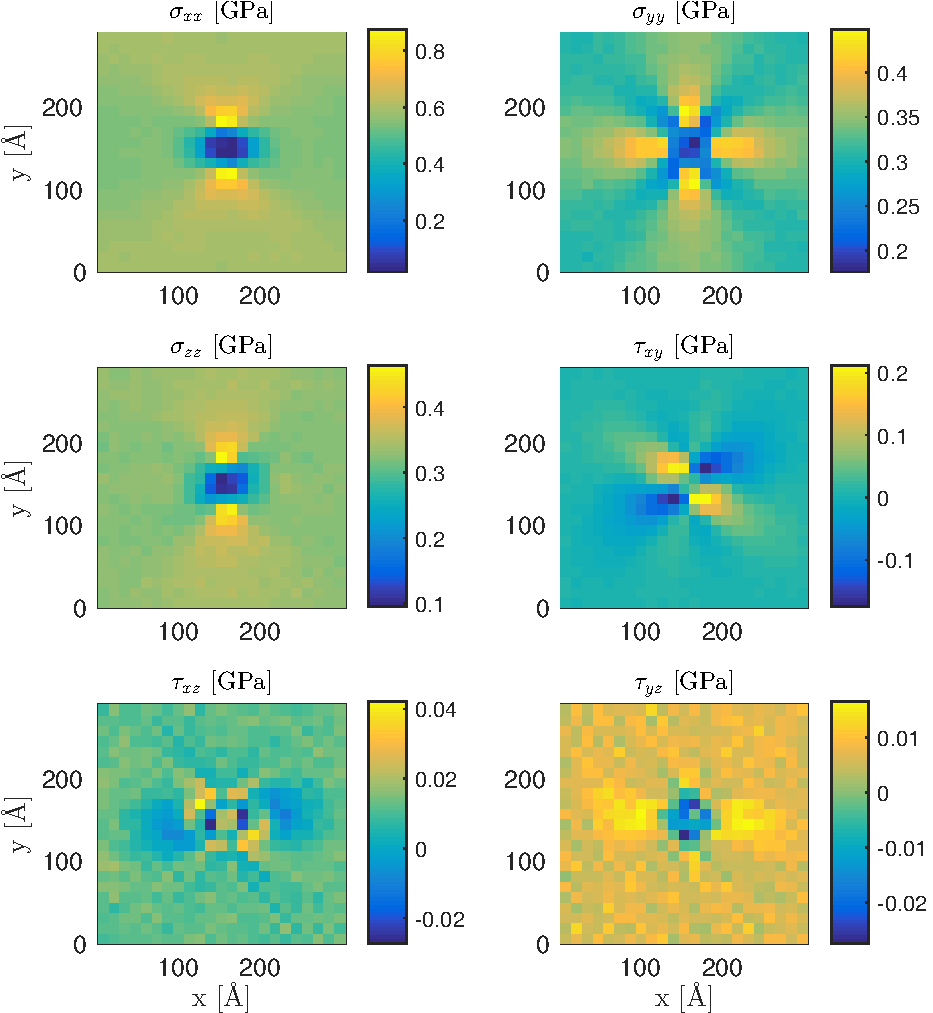
\includegraphics[width=\textwidth]{../figures/thesis/stressfield_avg_wait_for_crack.pdf}
\caption{Stess field averaged over \SI{20}{\pico\second} just after straining was stopped, and while waiting for a crack to start. The modeled system is $24\times 24\times 12$ sI unit cells. The four uppermost panels show features qualitatively in line with the analytical solution of the stress field around the crack tip of elliptical hole in a linearly elastic and isotropic material. The shear stress components outside the $xy$-plane are relatively small compared to the components in the $xy$-plane, which means the plane strain condition is satisfied fairly well. The stress fields near the crack tips are, at least qualitatively, similar to the analytical solution for isotropic materials given in figure \ref{fig:analytic_stress}. Note also the stress $\sigma_{zz}$ it looks like $\sigma_{xx}$ due to $L_z$ being fixed, disallowing Poisson contraction.}
\label{fig:stressfield_avg_wait_for_crack}
\end{figure}


\begin{figure}
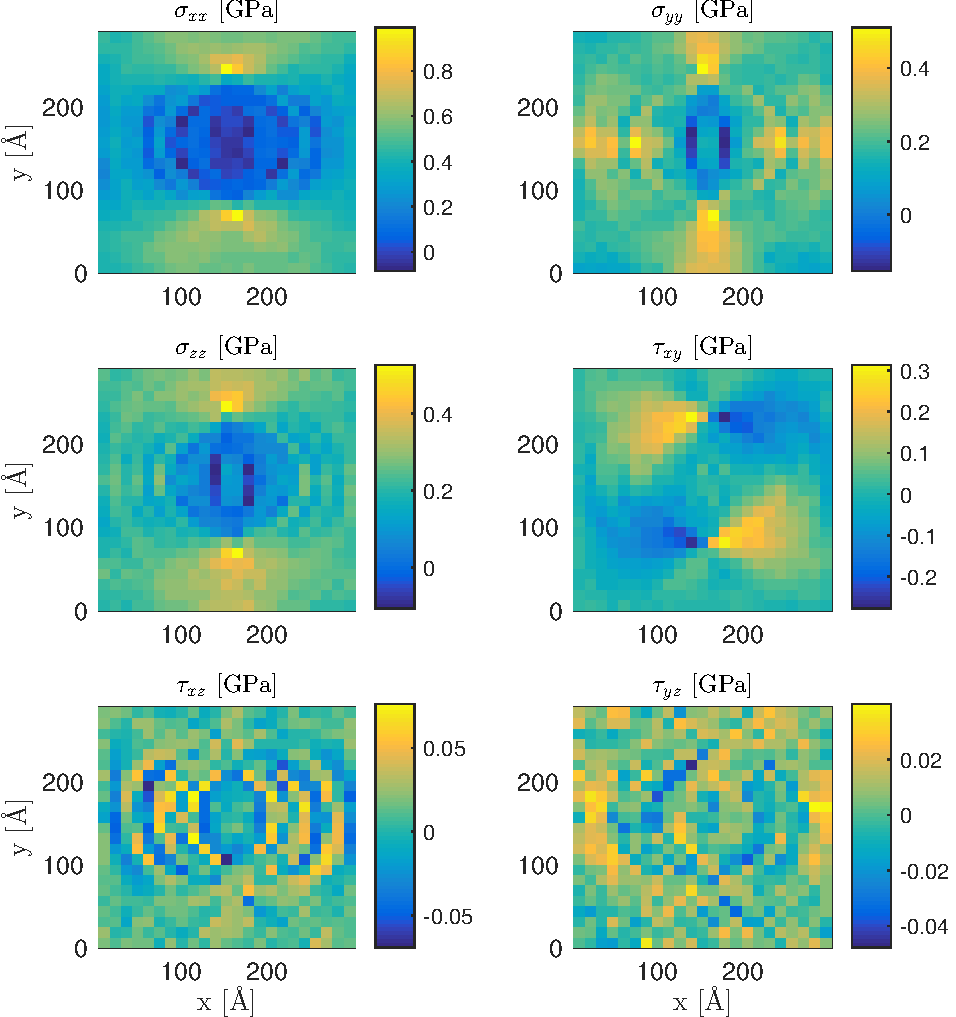
\includegraphics[width=\textwidth]{../figures/thesis/stressfield_snap_propagation_180.pdf}
\caption{Snapshot of stress field during crack propagation. Average over \SI{0.3}{\pico\second} before $t = \SI{180}{\pico\second}$.}
\label{fig:stressfield_snap_propagation_180}
\end{figure}


\begin{figure}
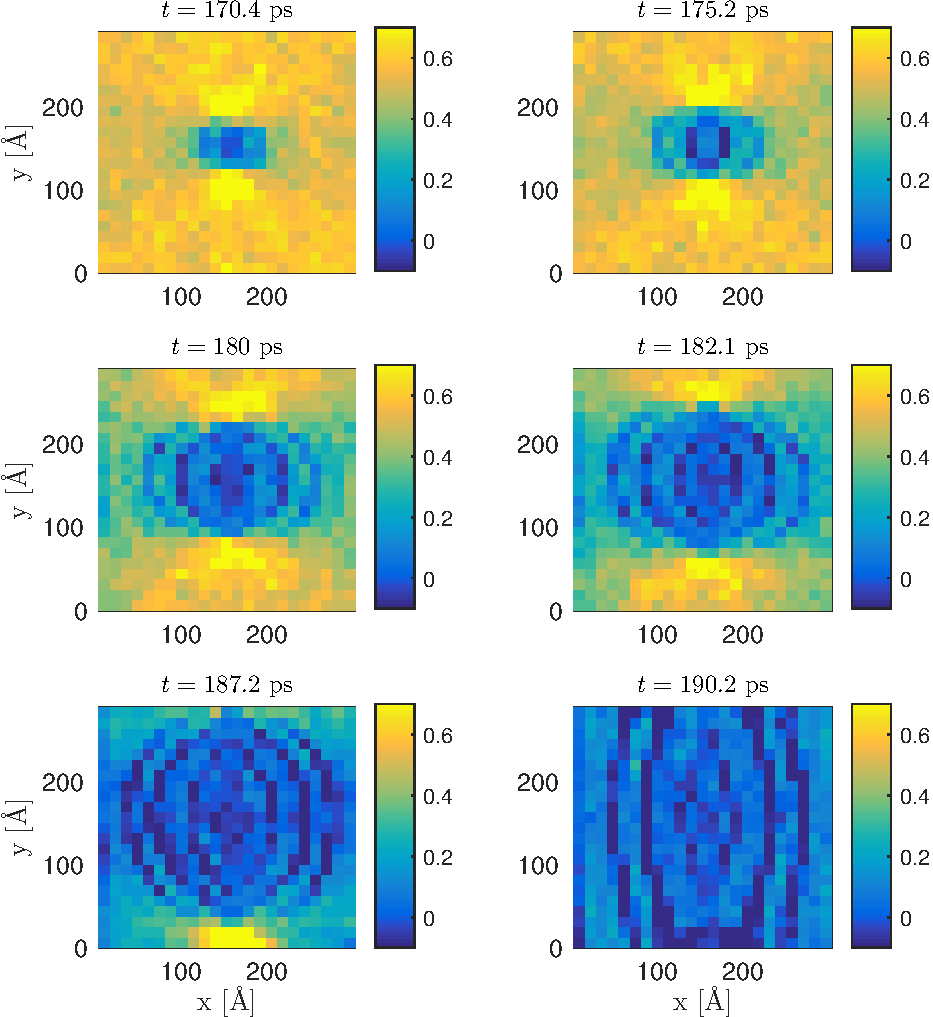
\includegraphics[width=\textwidth]{../figures/thesis/stressfield_timelapse.pdf}
\caption{Timelapse of the stress $\sigma_{xx}$ during crack propagation. There are clear signs of sound waves, and the shape of the waves indicate that the crack is traveling at a speed on the same order of magnitude as the shear wave speed. The color scale is kept equal among the simulations for easier comparison. For that reason, the stress near the crack tip is higher that what is available on the color scale. Notice that the two edges of the initial hole don't crack at the same time. The upper crack is leading the lower crack 
with $\sim \SI{10}{\angstrom}$. }
\label{fig:stressfield_timelapse}
\end{figure}




%%%%%%%%%%%%%%%%%%%%%%%%%%%%%%%%%%%%%%%%%%%%%%%%%%%%%%%%%%%%%%%%%%%%%%%%%%%%%%%%%%%%%
\section{A simple characterization of the fracture: The amount of free methane.}
%%%%%%%%%%%%%%%%%%%%%%%%%%%%%%%%%%%%%%%%%%%%%%%%%%%%%%%%%%%%%%%%%%%%%%%%%%%%%%%%%%%%%
I believe that the amount of free methane can be a valuable measure of how the crack surface looks because free methane no longer support a cage structure. Water molecules either stay on the crack surface, or are immediately drawn towards the crack surface in a matter of picoseconds after a crack has passed. Methane, on the other hand, is free to move in the pore space created by the crack. A first order approach to crack surface characterization is therefore to count free methane in the pore space and use that to estimate the amount of hydrate that was dissociated during fracture. The simplest estimate is obtained by using the hydrate number $n_w$ (5.75 for fully occupied sI hydrate) to count the amount of water molecules that are no longer part of the stable hydrate structure. 


\subsection{Estimate by counting}
\label{sec:freemethane_counting}
A more straightforward approach, which is more computationally demanding, is to go through all methane positions, and check whether they are part of the wall or the void, like what was done when tracking cracks. A particle is considered free if it was part of the void at any time during the simulation. The reason for the ``at any time during the simulation'' is that measuring frame by frame largely underestimates the number of free methane molecules. Methane molecules that are free are not necessarily far enough from the closest water molecule to be considered void, but they \emph{are} free to move. To check that the free methane molecules are indeed free, the positions of the methane molecules that were defined as void can be visualized at a point in time after the crack has propagated. Since free methane is accumulated in the measurement, a slightly higher $r_p$ is needed than for crack tracing -- near the lower reasonable limit for $r_p$, some improbable (but they will occur in large simulations) wall configurations will result in wall methane being counted as free. Figure \ref{fig:free_methane} is a snapshot of the system with the free methane molecules highlighted. Some of the methane molecules that are considered free actually reside in small cages near the fracture surface, and it is not obvious where they should be considered free or not. I tend toward considering the to be free, since they have proven that they are in cages that are not sufficiently intact to keep the methane molecules over time. Most of the free methane molecules are clearly free, so this should not be a big issue -- but it can be interesting to study for instance the rate at which methane is captured and released by the near-crack-surface cages.

\begin{figure}
\centering
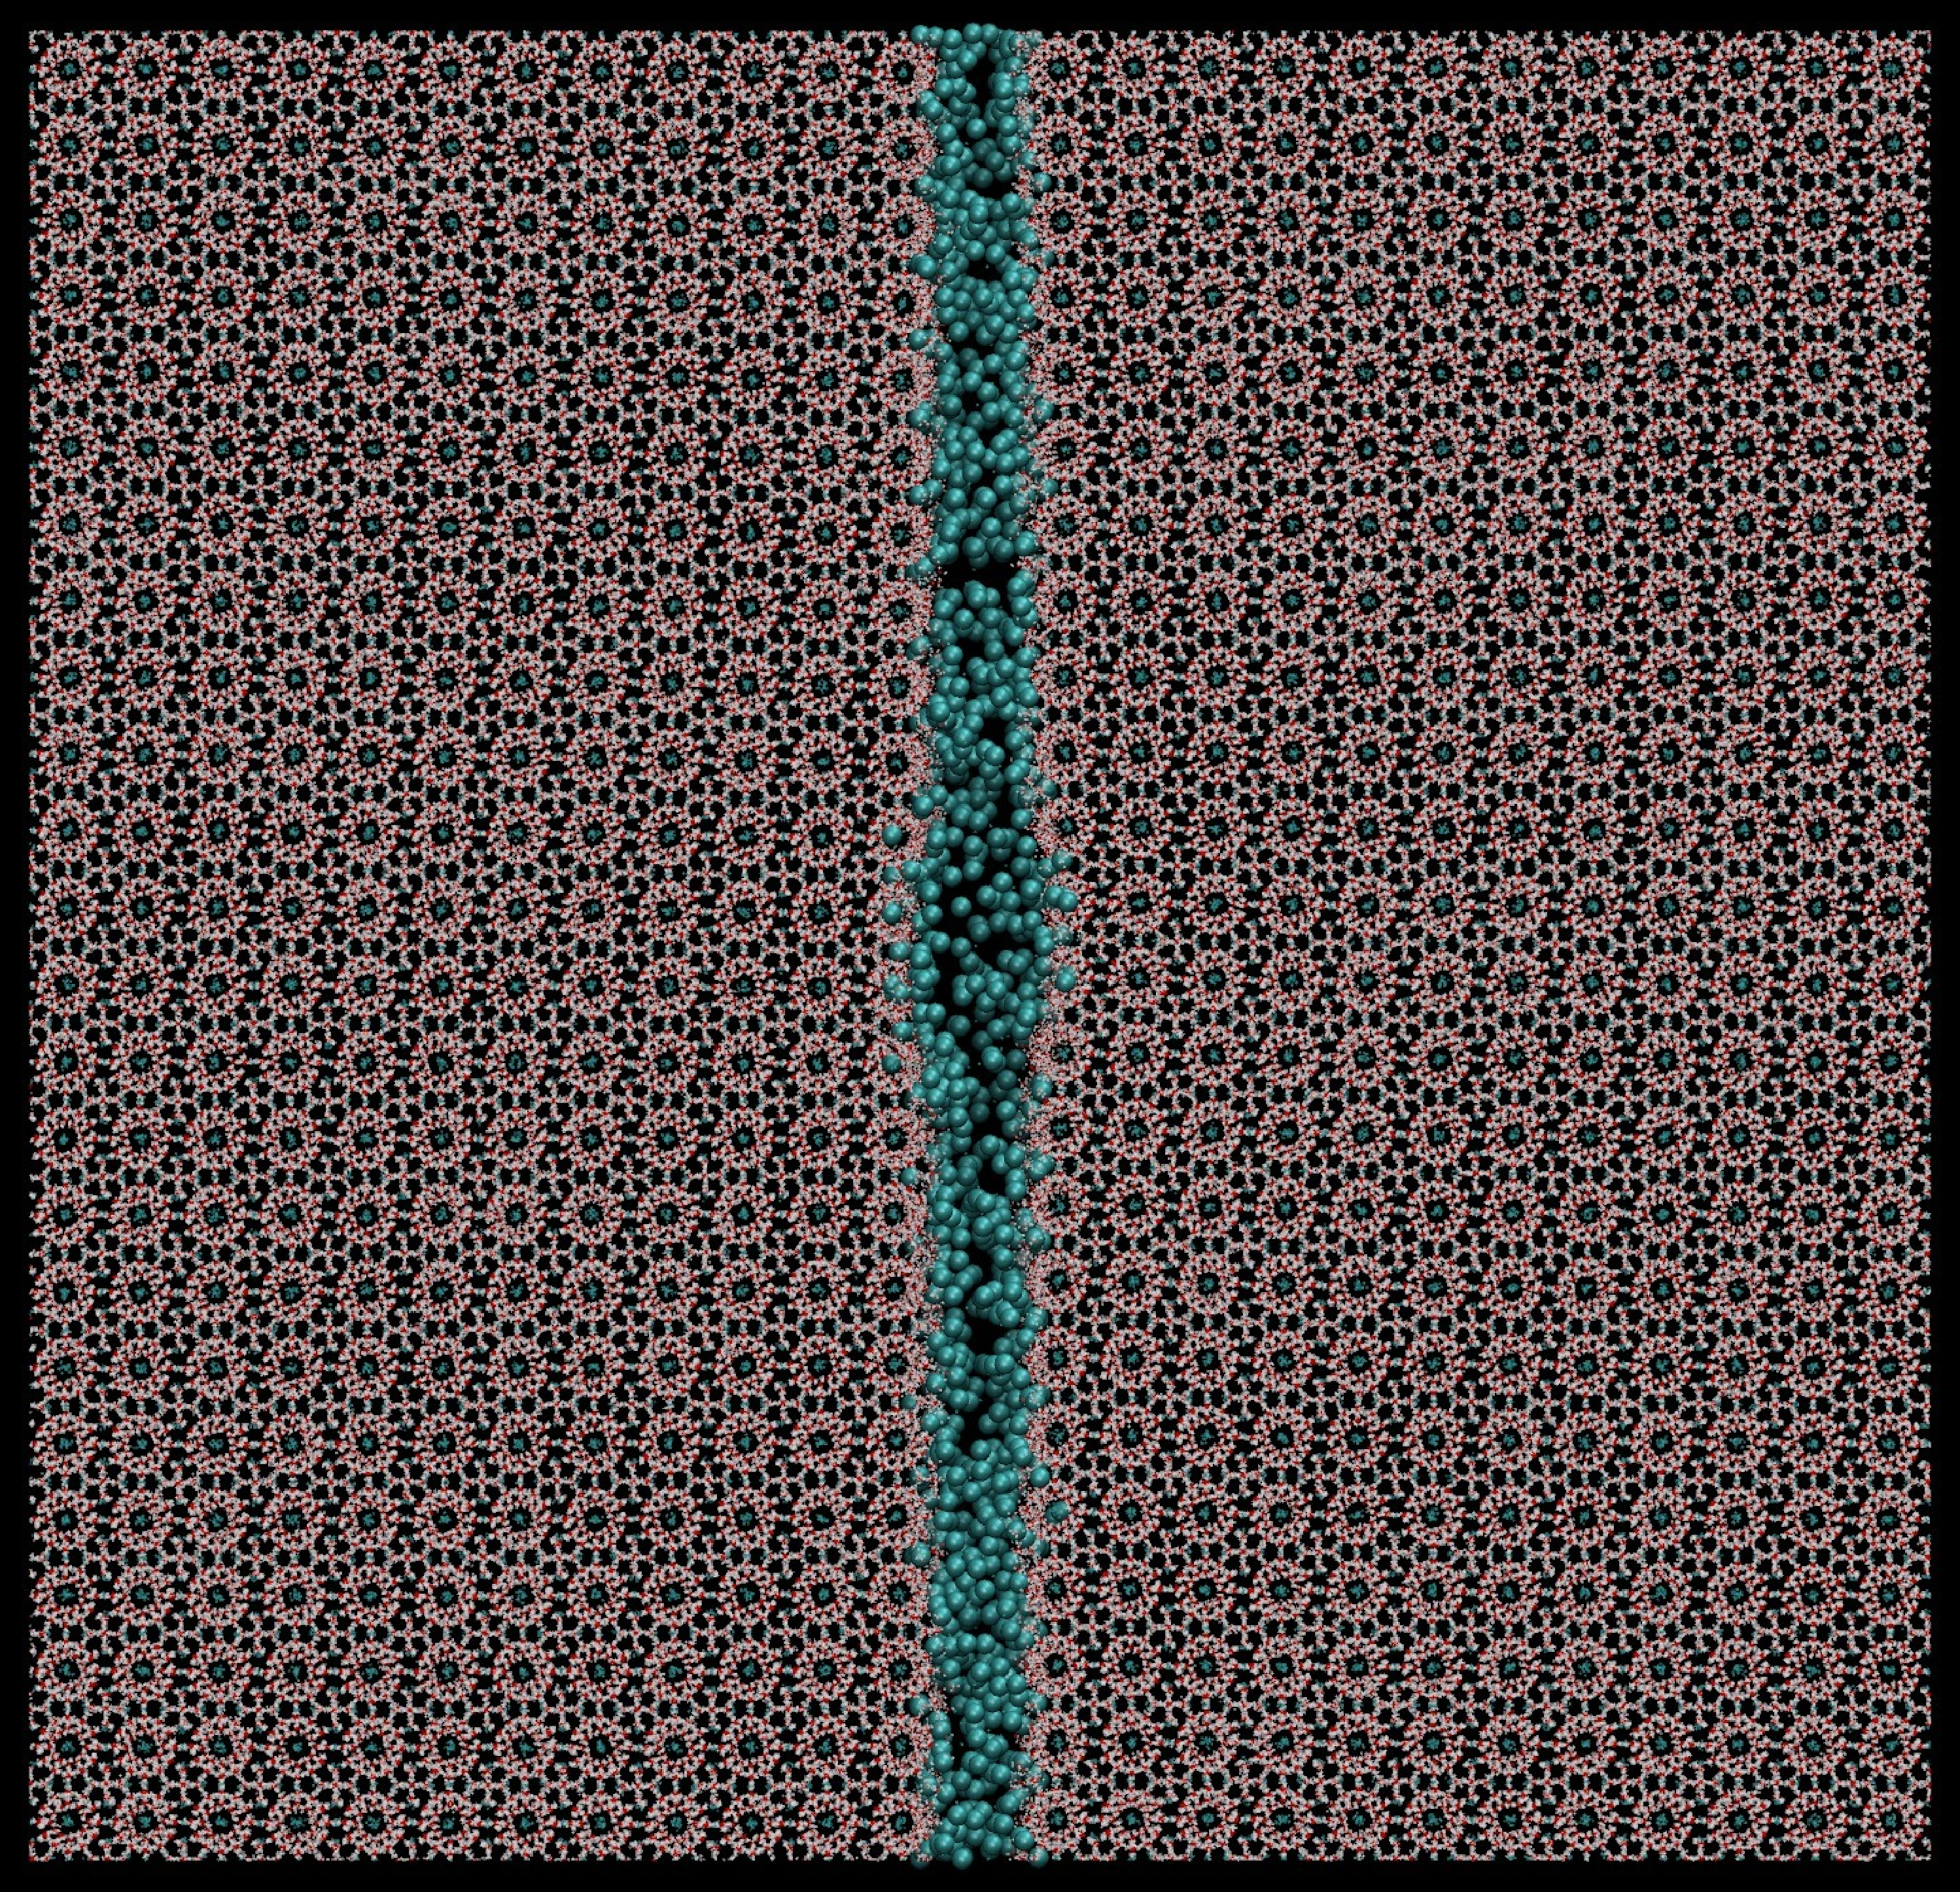
\includegraphics[width=\textwidth]{../pictures/free_methane.pdf}
\caption{Free methane -- particles that were more than $r_p = \SI{4.5}{\angstrom}$ away from any water molecule at some point -- are drawn as big green spheres. Other methane molecules are barely visible particles. Note that some ``free'' methane molecules actually occupy cages. Most of them are in the small nearest to the crack, but a few also occupy big cages, that are a bit farther from the crack surface. }
\label{fig:free_methane}
\end{figure}


\subsection{Results on free methane}
Figure \ref{fig:free_methane_diff_l} shows the amount of free methane during simulation for two different thicknesses of the system. The number of free methane molecules is rescaled using the number of sI unit cells per cross section parallel to the crack. With full occupancy, the number of methane molecules per sI cell is 8, and if a whole plane of unit cells released their methanes, that would yield a number of 8 free methanes after rescaling. The number of free methane molecules shows no significant variance with the system thickness. This is a bit surprising, since the crack propagation has seemed more jittery for thinner systems, which could have led to more methane being released. It might still be an effect, but in that case the effect must be small. 

\begin{figure}
\centering
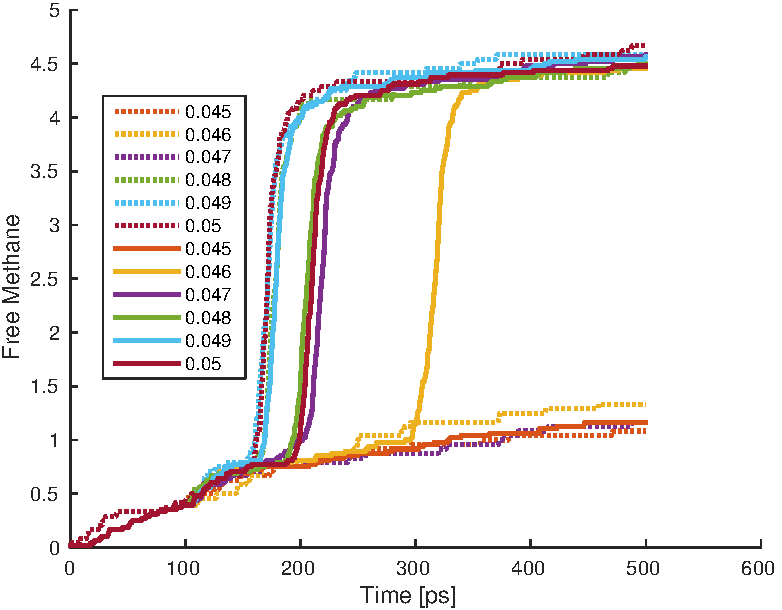
\includegraphics[width=10cm]{../figures/thesis/free_methane_nz1_nz2.pdf}
\caption{Free methane in time for systems with $L_z \approx \SI{12}{\angstrom}$ (dashed lines) $L_z\approx \SI{24}{\angstrom}$ (solid lines) for different values of the final strain (legend). Free methane is normalized by the number of unit cells in the fracture plane, so the plotted value is: $\text{Free Methane Molecules}\cdot L_{sI}^2/(L_yL_z)$.}
\label{fig:free_methane_diff_l}
\end{figure}

\subsection{Diffusion in the crack space}
Before I decided that counting the number of free methane molecules was a suitably good method to study free methane, I explored an indirect way of measuring the amount of free methane. The idea was to assume the motion of the free methane to be diffusive. The diffusion constant could then be measured and compare to what it would have been if all methane molecules were free to move. Unfortunately, the diffusion constant varies too much with the density of the methane gas for this to be a viable method -- both the number of methane molecules and the volume of the pore space is unknown. Furthermore, diffusion is not expected to be the same in pores as in a bulk Lennard-Jones fluid (see eg. \citet[p. 18]{Pozhar:1668293}. Therefore, this method was discarded. An additional problem is the global oscillations after crack propagation, which might further disturb the diffusion of particles. 

But, even though measuring the number of free methanes by mean squared displacement turned out to be difficult, the diffusion constant of the free methane can still be interesting to measure. Knowing the number of free methane molecules, and assuming the rest of the methanes have exhausted their potential for contribution to the mean squared displacement, the diffusion constant in the pore space can be measured. Figure \ref{fig:msq_methane_crack} shows the per-particle mean squared displacement of methane and water in the full-analysis simulation. The slope of the mean squared displacement is calculated to \SI{0.74}{\angstrom\squared\per\pico\second}, which corresponds to a diffusion coefficient of $D_E = \SI{1.2d-9}{\meter\squared\per\second}$. That value makes little sense, as it includes the enclathrated methane. When correcting for the fraction of methane molecules that are considered free to move, in this simulation it is 2.4 \%, the diffusion coefficient of the free methane is $D_E = \SI{5.3d-8}{\meter\squared\per\second}$. This value is probably an underestimation of the diffusion coefficient for the particles that are actually diffusing, as many methanes are trapped by the wall. What can be said, however, is that this is a very high diffusion coefficient, which, given the temperature, corresponds to a low pressure. A possible simulation to compare with, is a simulation by \citet{Cao2004} of Lennard-Jones methane in carbon nanotubes. At a temperature of \SI{267}{\kelvin}, they found self-diffusion coefficients for methane of around \SI{1d-8}{\meter\squared\per\second} to \SI{10d-8}{\meter\squared\per\second} for pressures ranging from \SI{1}{\mega\pascal} to \SI{8}{\mega\pascal}. The simulations were done in carbon nanotubes with diameters from \SI{20}{\angstrom} to \SI{40}{\angstrom}. This comparison is far-fetched, but it is reassuring that the results are in the right ballpark. It should be noted that the methane I observe in the crack is very dilute, possibly to the extent where Knudsen diffusion is a reasonable approximation. The methane being dilute is not obvious from the pictures of the system, since methanes that are behind each other seem to crowd the crack. If looking at the thinner system $L_z \approx \SI{12}{\angstrom}$, the diluteness becomes clear.

\begin{figure}
\centering
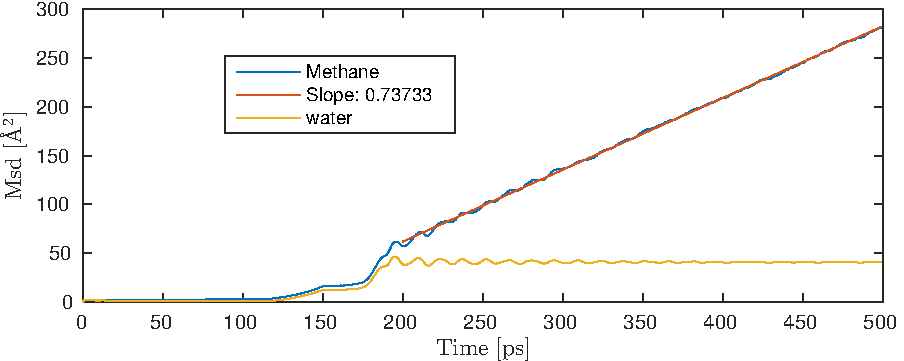
\includegraphics[width=14cm]{../figures/thesis/methane_crack_diffusion.pdf}
\caption{Per-particle mean squared displacement of methane and water in the full-analysis simulation. The slope of the methane mean squared displacement is $\SI{0.74}{\angstrom\squared\per\pico\second}$.}
\label{fig:msq_methane_crack}
\end{figure}

%%%%%%%%%%%%%%%%%%%%%%%%%%%%%%%%%%%%%%%%%%%%%%%%%%%%%%
\section{Increasing the temperature}
%%%%%%%%%%%%%%%%%%%%%%%%%%%%%%%%%%%%%%%%%%%%%%%%%%%%%%
All simulations until now have been run at $T=\SI{260}{\kelvin}$. This is a relatively low temperature, and specifically, it is lower than the melting point of water for the TIP4P/ICE water model. I start by running a few simulations in the large system, $24\times 24\times 12$ sI unit cells, and report results. Based on these results, I will decide whether a further investigation of temperature changes is warranted.

The new simulations are run at a temperature \SI{280}{\kelvin}, which is higher than the melting point of the TIP4P/Ice water model. 

Since the total crack area is limited by the cross-sectional area of the simulation box, I choose to look at the amount of free methane in these simulations. Figure \ref{fig:released_methane_temp} shows the amount of free methane in simulations with varying values of the strain level, and two different temperatures. It is clear that the amount of free methane gets higher when the temperature gets higher, but it is unclear whether the amount freed \emph{during} fracture is different. The clearest tendency is that methane is freed more quickly before and after crack propagation when the temperature is higher. 

\begin{figure}
\centering
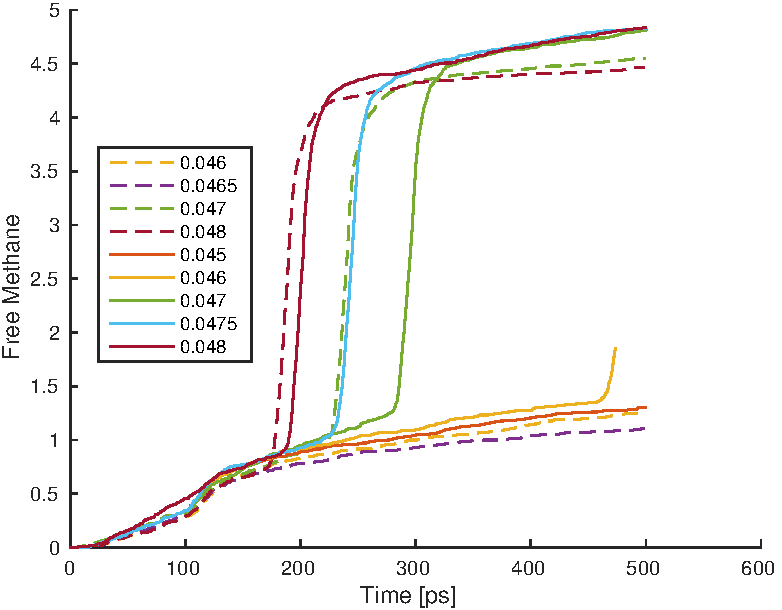
\includegraphics[width=12cm]{../figures/thesis/released_methane_temp.pdf}
\caption{Released for different strain levels with $T = \SI{260}{\kelvin}$ (dashed lines) and $T = \SI{280}{\kelvin}$ (solid lines). The amount of free methane gets significantly higher with the increased temperature.}
\label{fig:released_methane_temp}
\end{figure}

\section{Effects of the system thickness}
The study of finite size effects has not yet gotten much attention in this work, but from visual inspection of simulations with different thicknesses $L_z$, it is clear that there are finite thickness effects. Until now, three system sizes has been studied: A thickness of one sI unit cell, two sI unit cells, and a thickness of 12 sI unit cells. 

Most notably, the crack propagation in the thickest system seems more predictable than that in the thinnest system. Particularly, the crack tip in the small simulations can change direction for a short time, and then continue propagating in the y-direction but in another column of unit cells than it did before. Similar behavior has not been observed in the large system.

To systematically study this effect, I have compared the crack surface area in simulations with systems of different thicknesses, but with the same strain rates. A chaotic crack should leave a larger crack surface area than a straight one.

The result is that i cannot see any effect of the system thickness on the crack area; potential differences are masked by the fluctuations in the measured crack surface area.

\section{Investigating simulations with no system-spanning crack}
All simulations up to now has had a production time of \SI{400}{\pico\second}, but as there is a waiting time before fracture starts, there might be potential of having fracture in the non-fractures systems if the simulation is sufficiently long. It is also possible that something else will happen. The crack can for example change shape and strengthen the sample. It is also possible that a much slower crack can propagate, possibly not reaching the periodic boundary if the strain does not contribute enough energy to open a surface spanning the whole $yz$-plane. 

In this section, I look at a simulation very similar to the one described in section \ref{sec:complete_analysis_single_simulation}. The only difference is that the strain level after \SI{150}{\pico\second} is 0.045, and the temperature is \SI{280}{\kelvin}. No system spanning crack is observed during the \SI{400}{\pico\second} after straining. There is, however, a small increase in the surface area, as can be seen from the orange dotted line in the lower panel of figure \ref{fig:area_speed_stress_zoom}.

Since the system doesn't seem tom have equilibrated (the potential energy is still falling), I continue the simulation for another \SI{400}{\pico\second} to see what happens. Figure \ref{fig:crack_no_propagate_long_time_snapshots} shows images of the crack at selected points in time, and shows that even though the crack does not span the system after the simulations, it \emph{does} develop. It seems like the system is trying to minimize its mechanical energy by creating an optimal surface -- it looks like the crack is trying to optimize its shape. This is probably a different process than the process leading to rapid crack initiation and propagation. It can for instance be that the process can bee usefully described with a thermal activation and a stress activation. 

\begin{figure}
\begin{minipage}[b]{0.24\linewidth}
\subcaptionbox{$t=\SI{150}{\pico\second}$}{
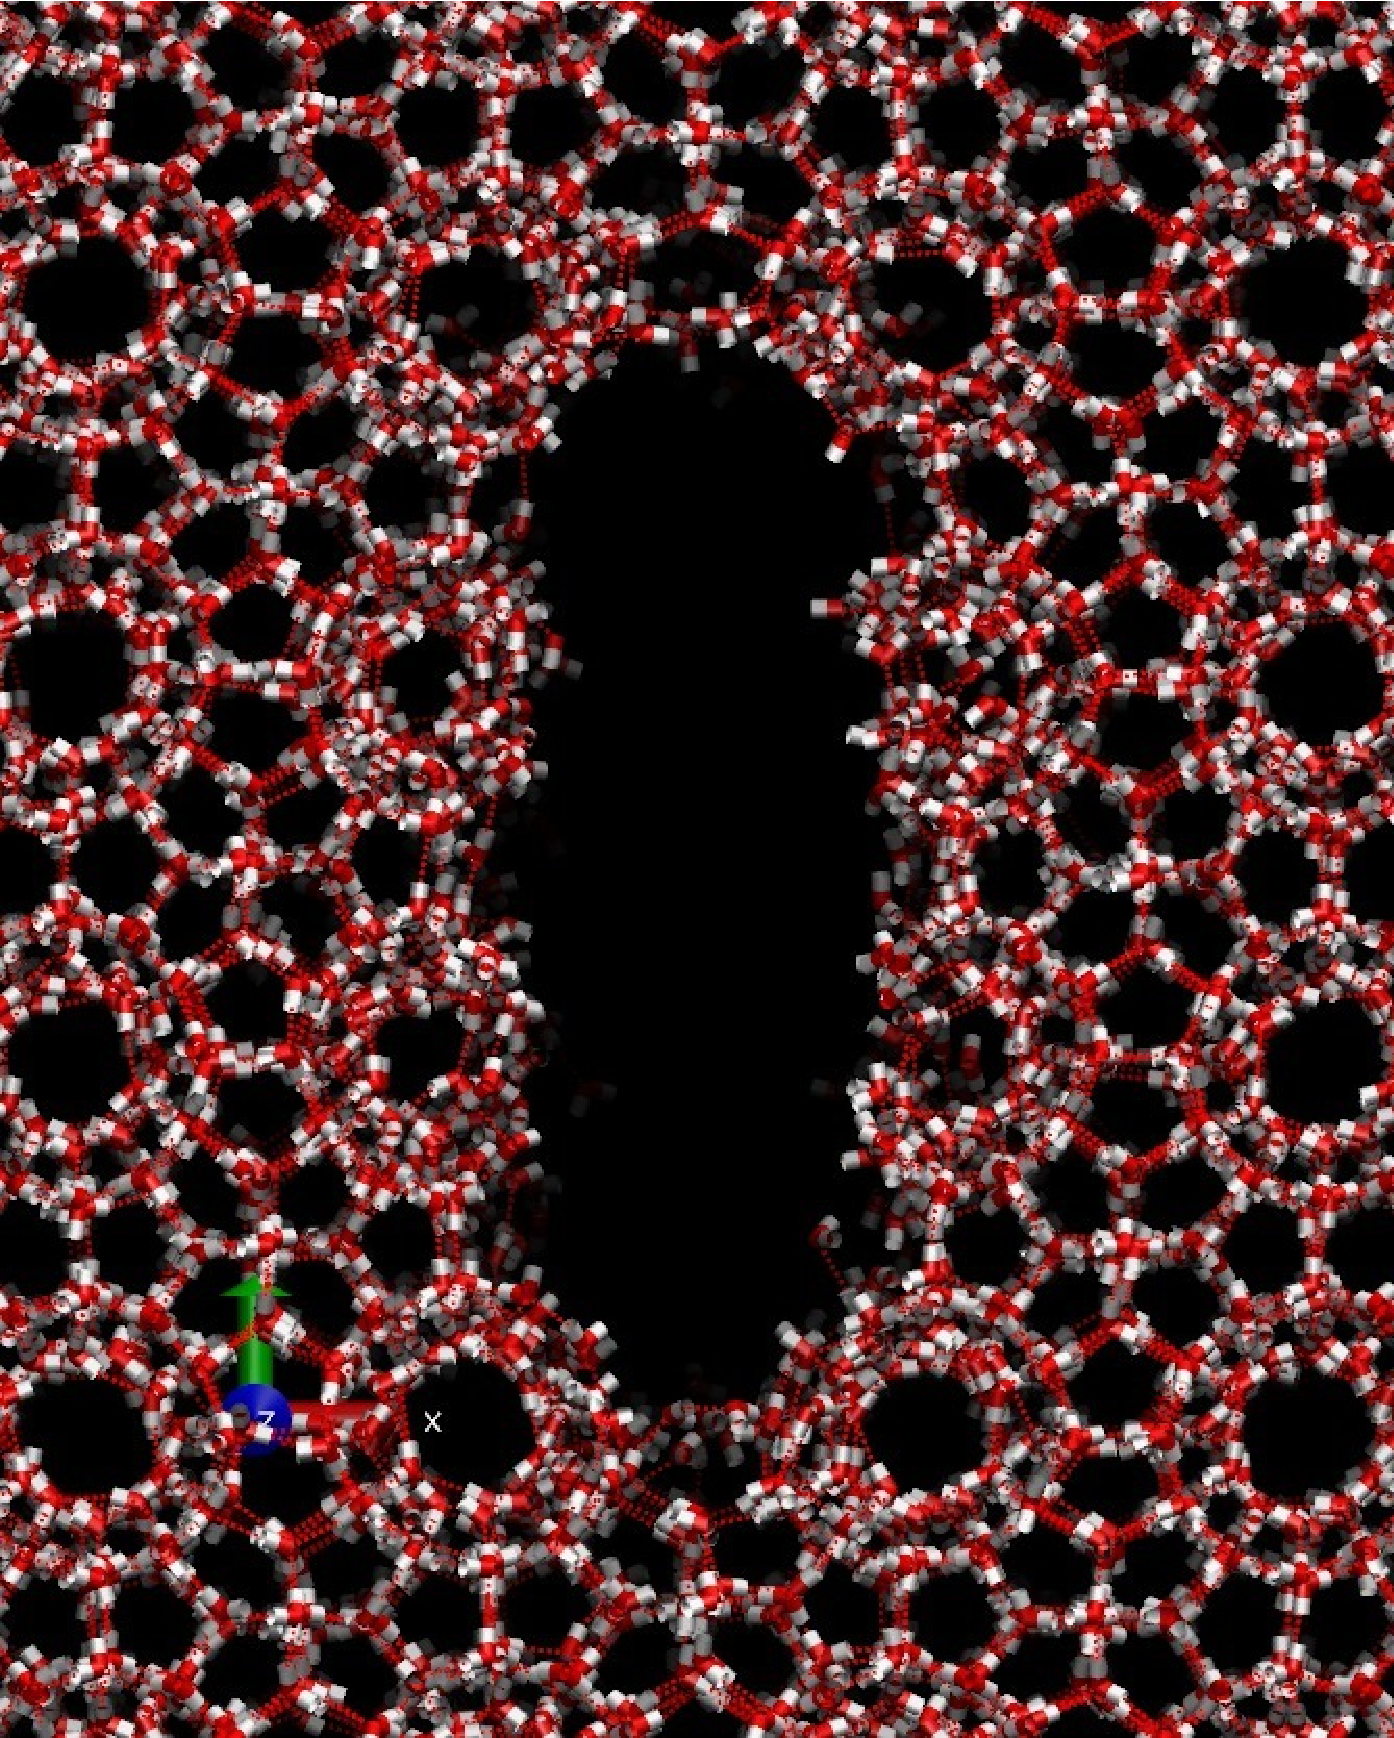
\includegraphics[width=\linewidth]{../pictures/snapshots_1045_280K/t_150000.pdf}}
\end{minipage}
\begin{minipage}[b]{0.24\linewidth}
\subcaptionbox{$t=\SI{300}{\pico\second}$}{
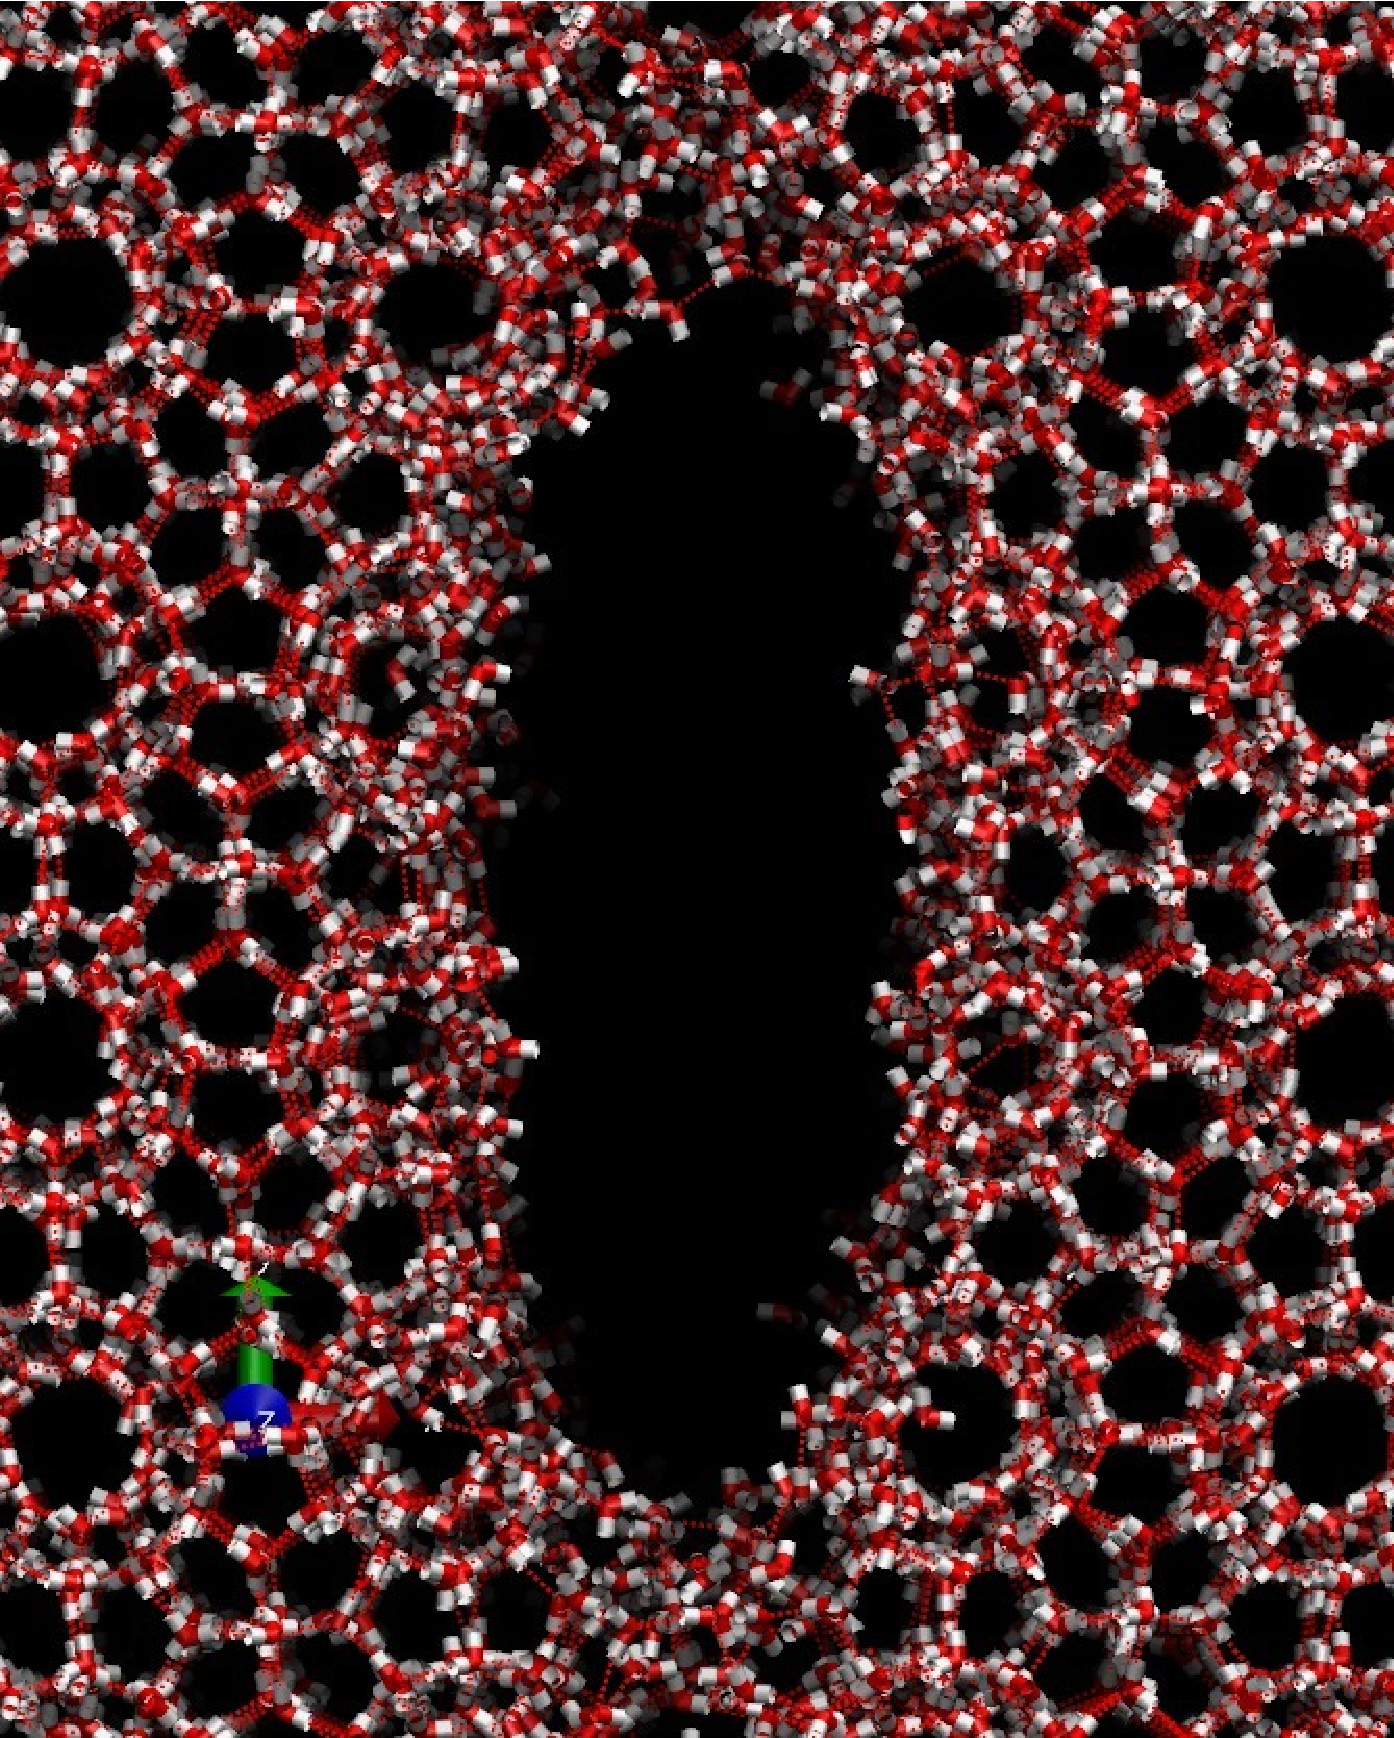
\includegraphics[width=\linewidth]{../pictures/snapshots_1045_280K/t_300000.pdf}}
\end{minipage}
\begin{minipage}[b]{0.24\linewidth}
\subcaptionbox{$t=\SI{600}{\pico\second}$}{
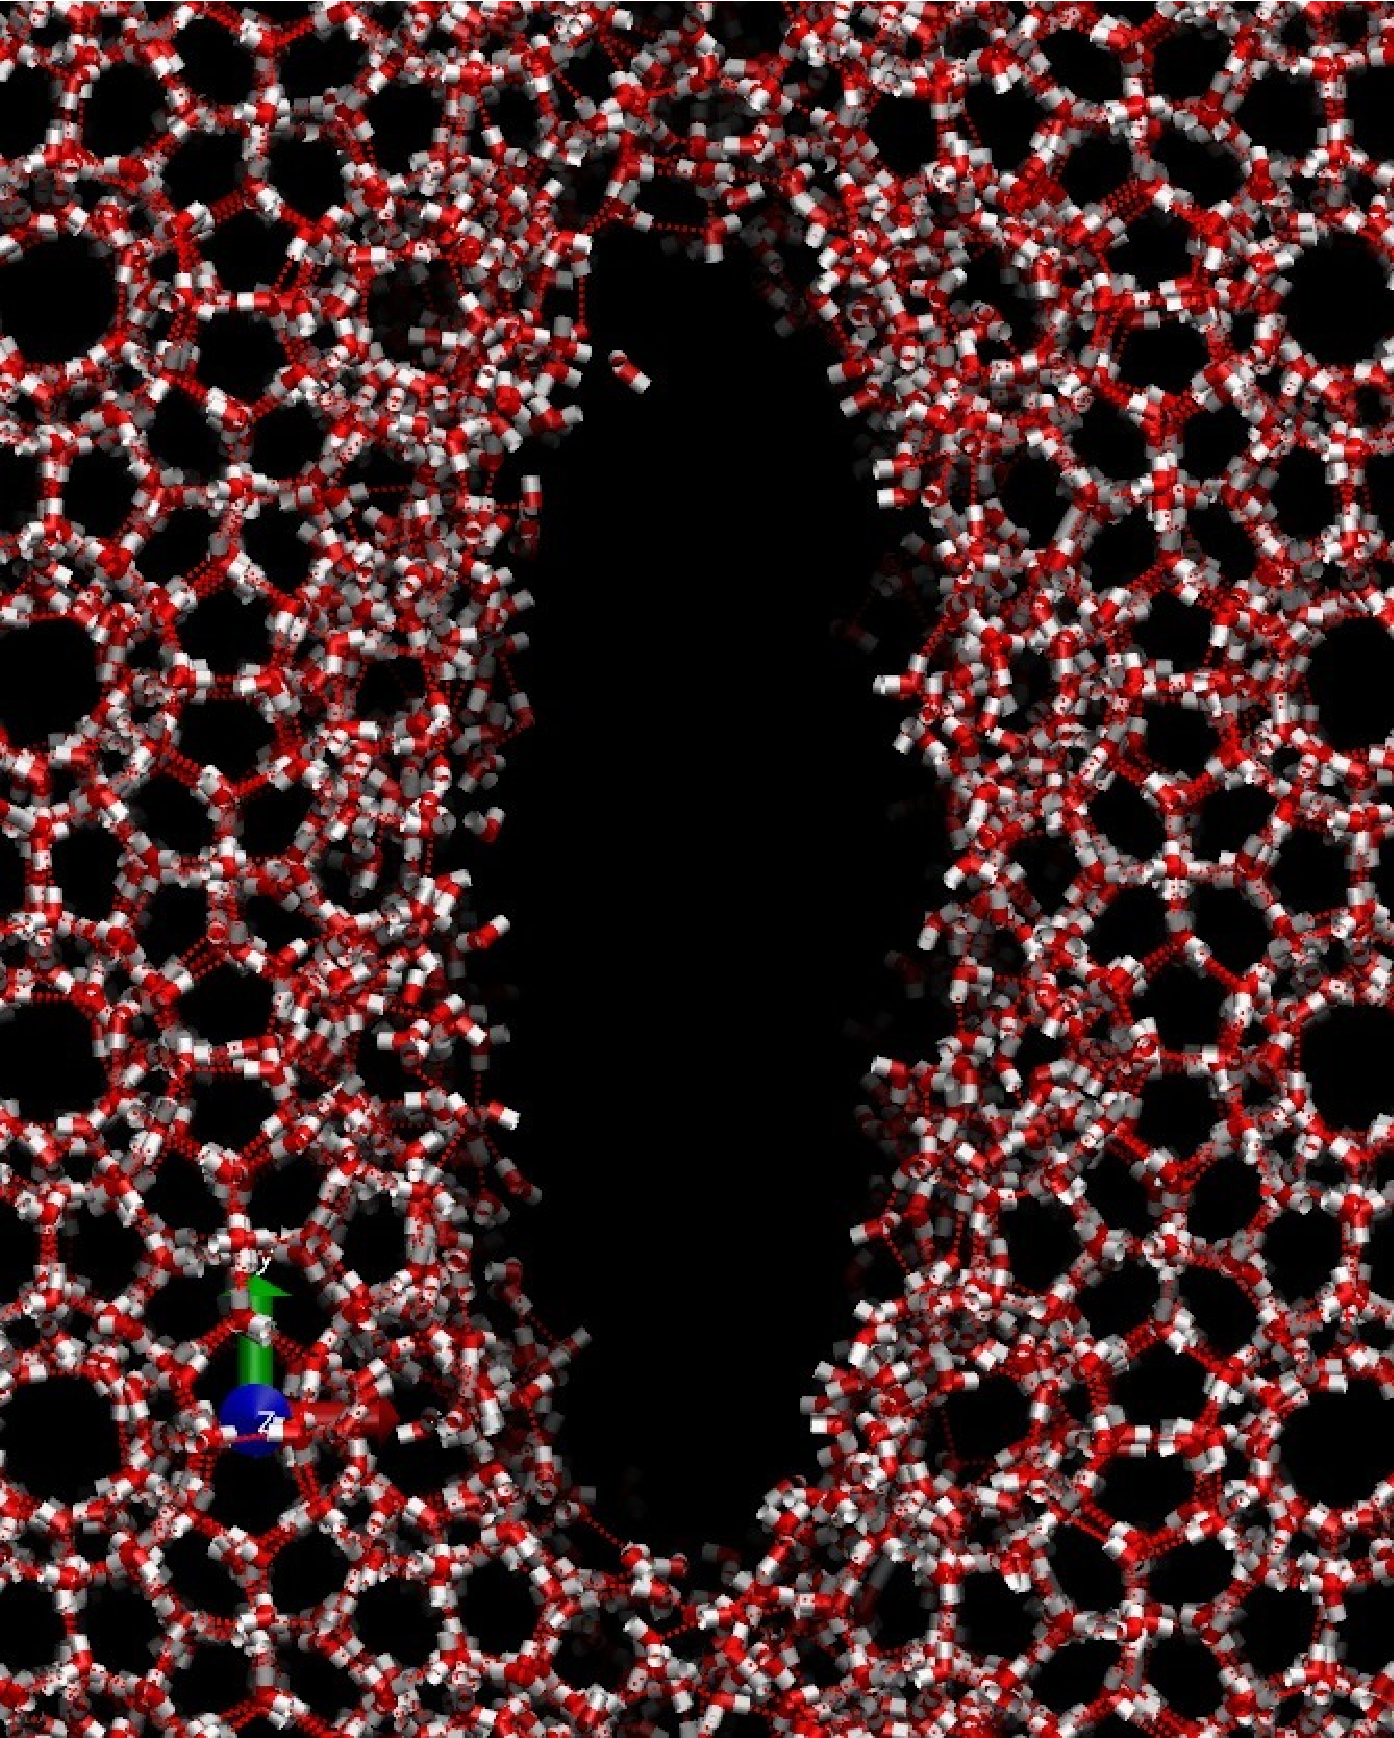
\includegraphics[width=\linewidth]{../pictures/snapshots_1045_280K/t_600000.pdf}}
\end{minipage}
\begin{minipage}[b]{0.24\linewidth}
\subcaptionbox{$t=\SI{900}{\pico\second}$}{
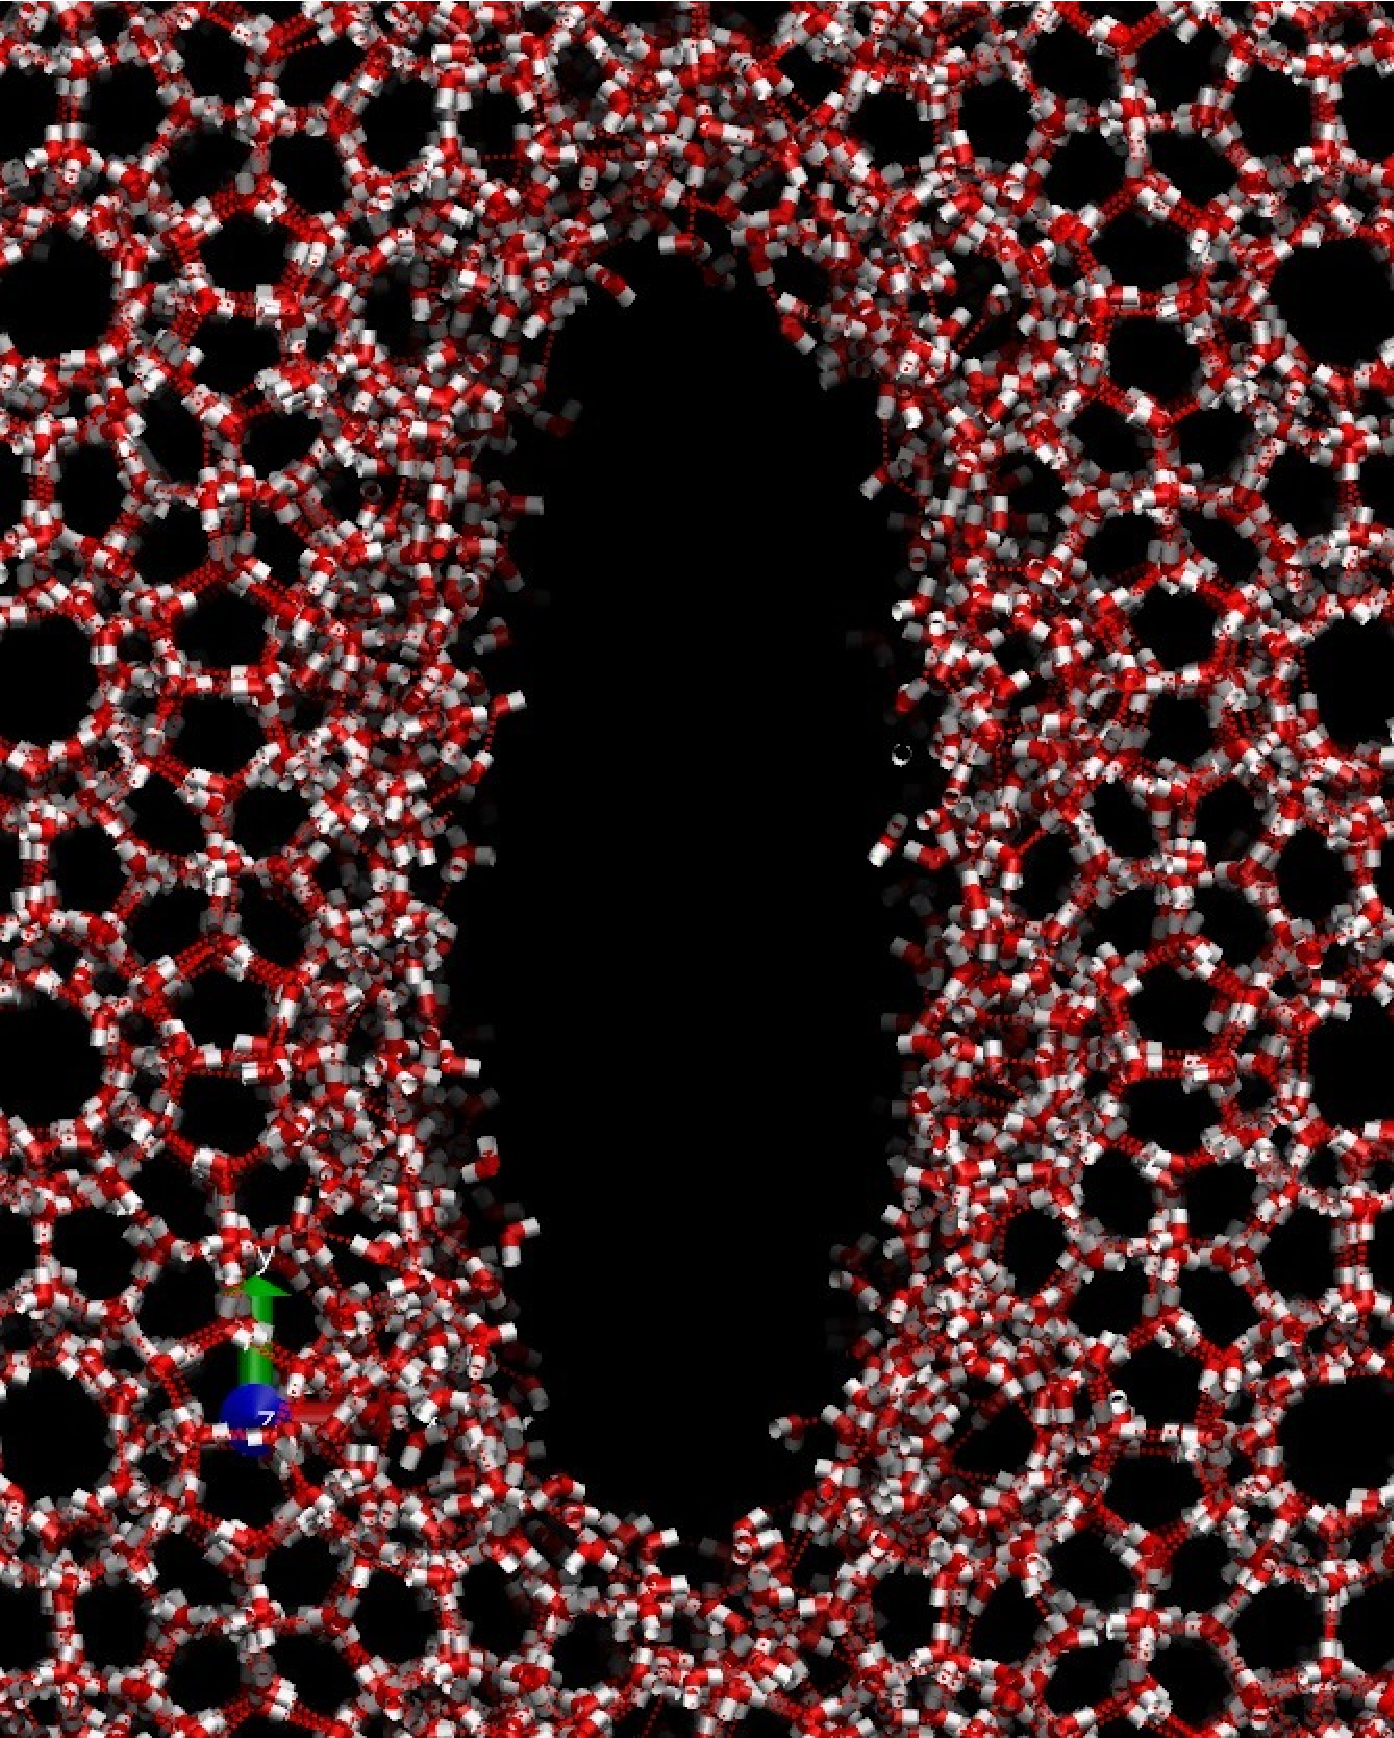
\includegraphics[width=\linewidth]{../pictures/snapshots_1045_280K/t_900000.pdf}}
\end{minipage}
\caption{Images zoomed in on the initial crack at different points in time in a long simulation. Methane molecules are hided for a better visual experience of the water. No global crack propagates, but there is still development of the small initial crack. From $t= \SI{150}{\pico\second}$ to $t=\SI{900}{\pico\second}$ the water-rich region at the wall-void interface is getting less ordered, and after $t=\SI{900}{\pico\second}$ there is a water-film between the sI hydrate and the free methane in the crack.}
\label{fig:crack_no_propagate_long_time_snapshots}
\end{figure}

\section{Aggregated results}
In this section, I present overall tendencies that arise from putting together the results I have already presented with results from additional simulations of the same kind, but with different strain levels. I end the section with a comparison of my results with the theory of linear elastic fracture mechanics.

\subsection{Waiting time for fracture}
In the simulations with $T=\SI{260}{\kelvin}$, the waiting time was short for the highly strained samples, and the samples subjected to too little strain didn't fracture. Between these extremes, there was no general rule that higher strains gave shorter waiting times. The simulations with $T=\SI{280}{\kelvin}$, on the other hand, showed more systematic behavior, and generally shorter waiting times. It is possible that the variation in waiting time is smaller when temperature increases, and especially when exceeding the melting temperature of pure water in the given model.

\begin{figure}
\centering
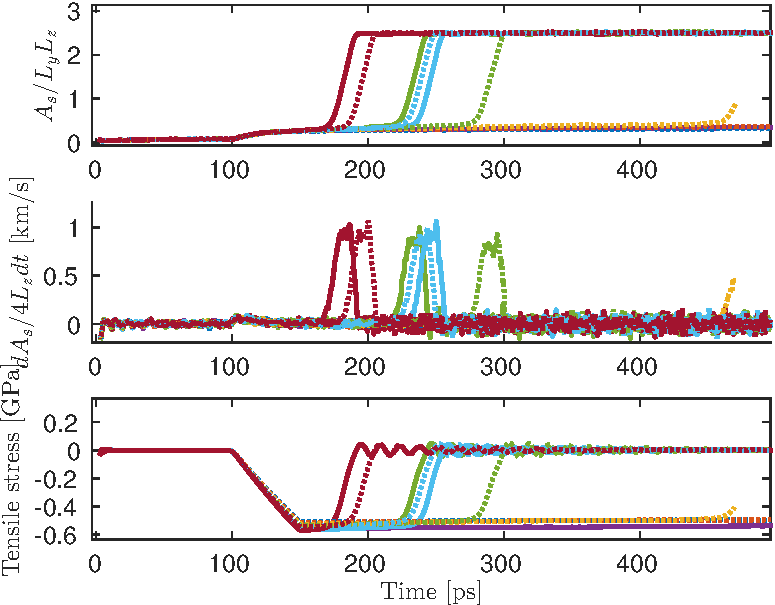
\includegraphics[width=12cm]{../figures/thesis/area_speed_stress_all.pdf}
\caption{Crack area (top panel), crack speed (middle panel) and tensile stress (lower panel). Simulation temperatures are \SI{260}{\kelvin} (solid lines) and \SI{280}{\kelvin} (dashed lines). Strains: 0.044 (blue) 0.045 (orange), 0.046 (yellow), 0.0465 (violet), 0.047 (green), 0.0475 (cyan), 0.048 (cardinal red). The colors are the same as in the legend of figure \ref{fig:fracture_theory_compare}. }
\label{fig:area_speed_stress_all}
\end{figure}

\begin{figure}
\centering
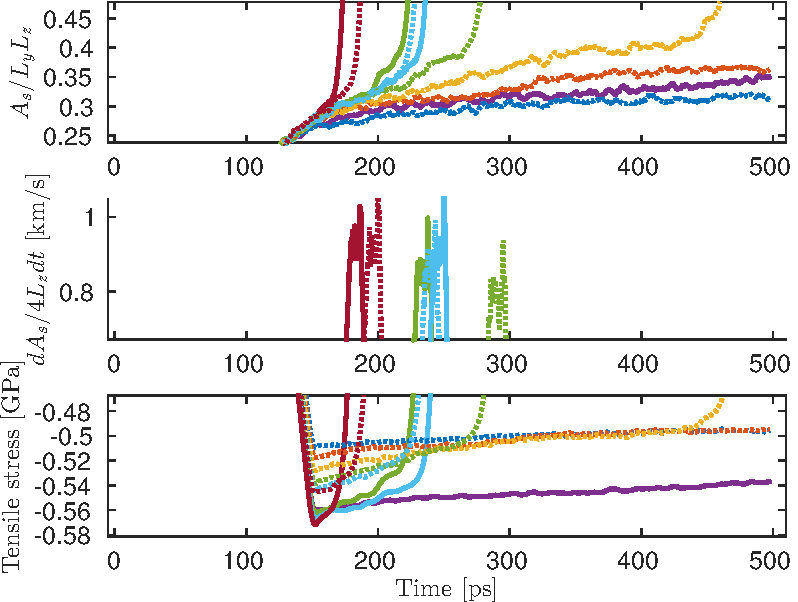
\includegraphics[width=12cm]{../figures/thesis/area_speed_stress_all_zoomed.pdf}
\caption{Crack area (top panel), crack speed (middle panel) and tensile stress (lower panel). The panels are the same as the ones in \ref{fig:area_speed_stress_all}, but they are significantly zoomed.}
\label{fig:area_speed_stress_zoom}
\end{figure}

\subsection{Crack tip speed}
Crack tip speeds have been measured both in the thin and the thick systems, but I have only made comparisons between different simulations for the thickest system. There is a clear tendency that the crack tip speed upon rupture increases with increasing strain level before crack propagation. This is unsurprising. The low accuracy of the speed measure makes is hard to make quantitative comparisons, and a longer system is probably needed for robust quantitative comparison. What can be said, is that even though the crack tip speed significantly depend on the strain, the differences in crack speed are not big. In figure \ref{fig:area_speed_stress_zoom}, all crack speeds fall roughly between \SI{750}{\meter\per\second} and \SI{1000}{\meter\per\second}. In terms of Rayleigh wave speeds, this range corresponds to $\approx 0.5 - 0.65 v_R$ (see table \ref{tbl:mechanical_from_simulation} for wave speeds in this model). This is well within the speed range where crack instabilities are expected to be present, but crack instabilities have not been prominent in the simulations in this work.
\subsection{Free methane}
Methane is freed almost instantly during crack propagation, which is opposed to the possibility of a very sharp crack where methane would have to diffuse out of their cages after crack propagation. It is also worth noting that the proportion of methane that is freed during rapid surface area growth is of the same order as the proportion of surface area that is grown during rapid area growth. That means methane is quickly released -- it does not stay in the hydrate lattice and then diffuse out.


\subsection{Surface energy and fracture toughness}
The same exercise of measuring the critical energy release rate of the hydrate as in section \ref{sec:energy_considerations} has been done for other system thicknesses and for the increased temperature. I have also read off the corresponding surface energy from figures like figure \ref{fig:pot_strain_eng_l1}. Since the surface energy is fluctuating, these results are uncertain, but they can at least be used to say that the critical energy release rate is approximately two times the surface energy, which classifies the hydrate as brittle. The results are summarized in table \ref{tbl:fracture_surface}. Since the surface energy in this work is gotten by simply checking the potential energy difference, it is unclear what it means. The free methane filling the crack can contribute energy that should probably rather be included in the crack-driving energy than in the crack-resisting energy, but I have not been investigating this possible effect. Since the free methane + ice system has a lower density than the methane hydrate, methane is likely to contribute to driving cracks. The tendency that the surface energy is higher than half the energy release rate for the high temperature system is quite robust, indicating that the pore methane is indeed playing a role.

\begin{table}
\centering
\caption{Surface energies and critical energy release rates from this work. The critical energy release rates must be taken as upper estimates, since a finer resolution in the strain increments could reveal lower strains supporting crack propagation.}
\label{tbl:fracture_surface}
\begin{tabular}{c|c|c}
Parameters & Surface energy & Critical energy release rate \\
\hline
\SI{260}{\kelvin}, $L_Z = \SI{12}{\angstrom}$ &\SI{0.19}{\joule\per\meter\squared} & \SI{0.42}{\joule\per\meter\squared} \\
\SI{260}{\kelvin}, $L_Z = \SI{24}{\angstrom}$ &\SI{0.20}{\joule\per\meter\squared} & \SI{0.37}{\joule\per\meter\squared} \\
\SI{260}{\kelvin}, $L_Z = \SI{144}{\angstrom}$ & \SI{0.20}{\joule\per\meter\squared} & \SI{0.40}{\joule\per\meter\squared}\\
\SI{280}{\kelvin}, $L_Z = \SI{145}{\angstrom}$ & \SI{0.21}{\joule\per\meter\squared} & \SI{0.38}{\joule\per\meter\squared}
\end{tabular}
\end{table}

\section{Comparison with linear elastic fracture mechanics}
Figure \ref{fig:fracture_theory_compare} shows the global tensile stress in the thick simulations (12 sI unit cells in the $z$-direction) plotted against the crack length. The crack length is estimated as $A_s/2L_z$, which means the crack is assumed to be thin. This probably slightly overestimate the crack lengths, since the cracks are elliptical prior to crack propagation, but the differences between the simulations can still be robustly analyzed. Results are presented both for simulations at $T= \SI{260}{\kelvin}$ and at $T=\SI{280}{\kelvin}$. Along with the evolution of the simulations on the Stress--Crack-width axes, I have plotted three expected fracture criteria from linear elastic fracture mechanics: The Inglis formula, the Griffith formula, and the finite width-corrected Griffith formula. Respectively:
\begin{align}
\sigma_f & = \sqrt{\frac{E\gamma_s}{4a}} \\
\sigma_f & = \sqrt{\frac{2E\gamma_s}{\pi a}} \\
\sigma_f & = \sqrt{\frac{2E\gamma_s}{2W\tan\left( \frac{\pi a}{2W}\right)}}
\end{align}
 I have indicated in the figure where the crack evolution goes from slow (melting) to fast (fracture). This point is found by inspecting the crack speed plot, finding the time just before the crack tip speed starts to increase rapidly. This point in time is quite well-defined. The markers in figure \ref{fig:fracture_theory_compare} indicate the stress--crack-width configuration at this specific time for each simulation. 
 The results agree well with the Griffith theory for brittle solids. This plot can aid the understanding of two separate mechanisms for fracture. Some process slowly increases the crack width and reduces the tensile stress, until -- at some point -- the stress--crack-width configuration is such that it allows for rapid crack growth. This should be determined by whether the simulation follows a less steep slope than some critical line, which is probably close to the finite width Griffith line. The seemingly different slopes taken by the points of critical failure for the two different temperatures is still unexplained. I speculate that this can be attributed to the pressure of the methane in the initial crack, but I have not studied that in this work.
%
\begin{figure}
\centering
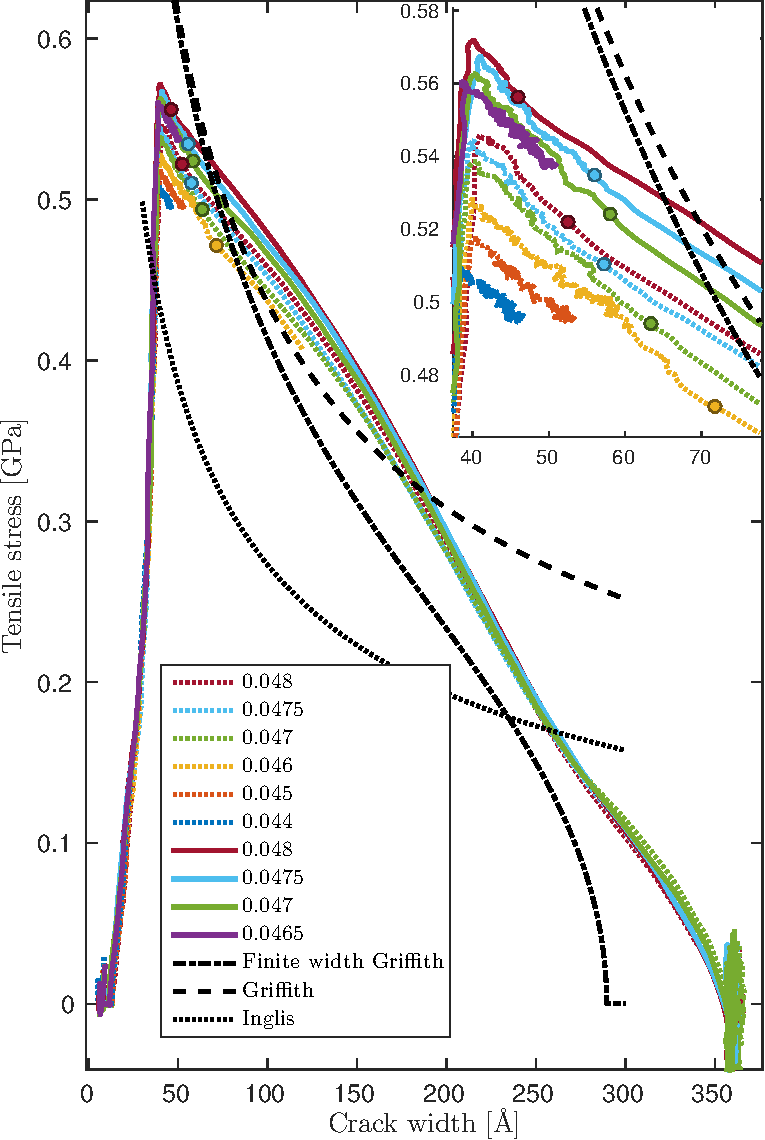
\includegraphics[width=12cm]{../figures/thesis/stress_area_lefm.pdf}
\caption{Relationship between tensile stress and crack width during dynamic runs. Markers indicate where critical fracture is estimated to have started (judgment call from looking at the fracture speed). It is the position of the markers that determine whether this is a good agreement with Griffith or Inglis theory. The crack length is estimated as $A_s/2L_z$, and it is clear that it is over-estimated at the end of the simulation (at full crack opening). It is not clear whether the crack length is over-estimated at the early stages of crack propagation. When straining is finished, which is at the point where the stress reaches its maximum, the crack area is quite exactly estimated to the length of the crack that was carved out, namely \SI{40}{\angstrom}. The theory curves (Inglis and Griffith) are calculated using $E=\SI{7.1}{\giga\pascal}$ and $\gamma_s = \SI{0.21}{\joule\per\meter\squared}$ The finite width curve is made using equation \ref{eq:griffith_finite_sheet}. The legend indicate the maximum strain level in each simulation, and the different theoretical curves.}
\label{fig:fracture_theory_compare}
\end{figure}